\noindent Cuatro simulacros de \textbf{150 minutos y diez puntos}. Son selecciones de entrenamiento del banco de problemas, con los mismos datos, no exámenes oficiales ni variantes inéditas. Los cuatro cubren conjuntamente los ocho temas; cada prueba combina cinco casos de varios capítulos. Las soluciones aparecen en la segunda parte.
\tableofcontents\mainmatter\part{Enunciados}


\chapter{Simulacro 1}

\objetivos{Trabaja sin consultar las soluciones; reserva 25 minutos por problema y 25 minutos para comprobaciones.}

Calculadora y una hoja propia de fórmulas permitidas. Cada problema vale 2 puntos: hipótesis y planteamiento, 0.5; desarrollo, 0.75; resultado con unidades, 0.5; comprobación e interpretación, 0.25. Penaliza un error arrastrado una sola vez si el procedimiento posterior es coherente. El tiempo y la rúbrica son propuestas de entrenamiento.

\par\medskip\noindent\begin{minipage}{\linewidth}

\section{Problema 1 · 2 puntos}

Un tirante de 2 m de longitud debe tener una rigidez axial $k = EA/L = 5\times 10^{7}$ N/m. Calcule su masa si es de aleación 7075 ($E = 71{,}7$ GPa, $\rho = 2810$ kg/m$^3$) y compare con la de un tirante de acero ($E = 200$ GPa, $\rho = 7900$ kg/m$^3$).

\par\medskip\noindent\begin{tabular}{@{}p{.18\linewidth}p{.26\linewidth}p{.48\linewidth}@{}}
\toprule Símbolo & Valor y unidad & Significado\\\midrule
$k$ & $50\,\mathrm{kN/mm}$ & rigidez axial\\
$L$ & $2.0\,\mathrm{m}$ & longitud\\
$E$ & $71.7\,\mathrm{GPa}$ & módulo de Young del 7075\\
$\rho$ & $2810\,\mathrm{kg/m^3}$ & densidad del 7075\\
\bottomrule\end{tabular}\par\medskip



\par\textbf{Hipótesis de trabajo.} barra prismática y homogénea; diseño gobernado por la rigidez axial; no se incluyen uniones.

\par\textit{Entrega: modelo, desarrollo, unidades y una comprobación. Caso del banco: PRB-0148.}\end{minipage}\par\medskip

\par\medskip\noindent\begin{minipage}{\linewidth}

\section{Problema 2 · 2 puntos}

Una barra de aleación 7075 ($E = 71{,}7$ GPa) de 20 mm de diámetro y $1{,}5$ m de longitud soporta una tracción axial de 60 kN. Calcule la tensión normal, la deformación y el alargamiento total, y compruebe que la tensión queda por debajo del límite elástico mínimo de 430 MPa.

\par\medskip\noindent\begin{tabular}{@{}p{.18\linewidth}p{.26\linewidth}p{.48\linewidth}@{}}
\toprule Símbolo & Valor y unidad & Significado\\\midrule
$F$ & $60000\,\mathrm{N}$ & tracción axial\\
$d$ & $0.02\,\mathrm{m}$ & diámetro\\
$L$ & $1.5\,\mathrm{m}$ & longitud\\
$E$ & $71.7\,\mathrm{GPa}$ & módulo de Young del 7075\\
\bottomrule\end{tabular}\par\medskip



\par\textbf{Hipótesis de trabajo.} tensión uniforme lejos de los extremos; material elástico lineal; pequeñas deformaciones.

\par\textit{Entrega: modelo, desarrollo, unidades y una comprobación. Caso del banco: PRB-0151.}\end{minipage}\par\medskip

\par\medskip\noindent\begin{minipage}{\linewidth}

\section{Problema 3 · 2 puntos}

Una viga biapoyada de 4 m de luz soporta una carga triangular que vale cero en el apoyo izquierdo $A$ y 9 kN/m en el derecho $B$. Calcule la reacción en $B$.

\par\medskip\noindent\begin{tabular}{@{}p{.18\linewidth}p{.26\linewidth}p{.48\linewidth}@{}}
\toprule Símbolo & Valor y unidad & Significado\\\midrule
$L$ & $4\,\mathrm{m}$ & luz\\
$q_{0}$ & $9\,\mathrm{kN/m}$ & carga máxima\\
\bottomrule\end{tabular}\par\medskip



\par\textbf{Hipótesis de trabajo.} viga isostática biapoyada.

\par\textit{Entrega: modelo, desarrollo, unidades y una comprobación. Caso del banco: PRB-0190.}\end{minipage}\par\medskip

\par\medskip\noindent\begin{minipage}{\linewidth}

\section{Problema 4 · 2 puntos}

Un cajón cerrado de línea media 120 \ensuremath{\times} 70 mm y pared de 2 mm está sometido a un par torsor de +2,1 kN·m a lo largo de 1,2 m. Calcule el flujo de Bredt, la tensión en la pared, J y el giro entre extremos. Dibuje los sentidos del flujo. Dato del material: G = 26 955 MPa. [E2-C05:w\_cajon\_uniforme]

\par\medskip\noindent\begin{tabular}{@{}p{.18\linewidth}p{.26\linewidth}p{.48\linewidth}@{}}
\toprule Símbolo & Valor y unidad & Significado\\\midrule
$M_{x}$ & $2100000\,\mathrm{N\,mm}$ & torsor positivo ULE\\
$G$ & $26955\,\mathrm{MPa}$ & módulo transversal\\
$L$ & $1200\,\mathrm{mm}$ & longitud de referencia\\
$t_{1}$ & $2.0\,\mathrm{mm}$ & inferior\\
$t_{2}$ & $2.0\,\mathrm{mm}$ & derecha\\
$t_{3}$ & $2.0\,\mathrm{mm}$ & superior\\
$t_{4}$ & $2.0\,\mathrm{mm}$ & izquierda\\
\bottomrule\end{tabular}\par\medskip

\par\medskip\noindent\begin{minipage}{\linewidth}\centering
\begin{tikzpicture}[>=Stealth]
\coordinate (A) at (0.00000,0.00000);
\fill (A) circle (1.5pt) node[above right,font=\small]{A};
\coordinate (B) at (4.50000,0.00000);
\fill (B) circle (1.5pt) node[above right,font=\small]{B};
\coordinate (C) at (4.50000,-2.62500);
\fill (C) circle (1.5pt) node[above right,font=\small]{C};
\coordinate (D) at (0.00000,-2.62500);
\fill (D) circle (1.5pt) node[above right,font=\small]{D};
\draw[->,very thick,studiumBlue] (A) -- (B) node[midway,fill=white,font=\small]{$t_1$};
\draw[->,very thick,studiumBlue] (B) -- (C) node[midway,fill=white,font=\small]{$t_2$};
\draw[->,very thick,studiumBlue] (C) -- (D) node[midway,fill=white,font=\small]{$t_3$};
\draw[->,very thick,studiumBlue] (D) -- (A) node[midway,fill=white,font=\small]{$t_4$};
\draw[->] (-1,.3)--(-.2,.3) node[above]{$z$};
\draw[->] (-1,.3)--(-1,-.5) node[left]{$y$};
\end{tikzpicture}
\par\small Nudos $(z,y)$ en mm: $A=(0,0)$; $B=(120,0)$; $C=(120,70)$; $D=(0,70)$.
\par\small Flechas: sentido positivo de $q(s)$; $s=0$ en el nudo inicial de cada pared.
\par\small Recorridos de célula: $A\to B\to C\to D$.
\par\normalsize\end{minipage}\par\medskip

\par\textbf{Hipótesis de trabajo.} torsión pura de Saint-Venant; sección prismática; paredes delgadas de línea media especificada; G homogéneo; torsor positivo antihorario en la cara vista según ULE.

\par\textit{Entrega: modelo, desarrollo, unidades y una comprobación. Caso del banco: PRB-0208.}\end{minipage}\par\medskip

\par\medskip\noindent\begin{minipage}{\linewidth}

\section{Problema 5 · 2 puntos}

Un panel aeronáutico está sometido a tensión plana con $\sigma_x$ = 140 MPa, $\sigma_y$ = 20 MPa y $\tau_{xy}$ = +45 MPa. Calcule las tensiones sobre un elemento girado 30 grados antihorarios, las tensiones principales y su orientación; dibuje el círculo de Mohr. Considere tracción positiva y $\tau_{xy}$ en la cara normal +x orientada hacia +y.

\par\medskip\noindent\begin{tabular}{@{}p{.18\linewidth}p{.26\linewidth}p{.48\linewidth}@{}}
\toprule Símbolo & Valor y unidad & Significado\\\midrule
$\sigma_{x}$ & $140\,\mathrm{MPa}$ & tensión normal x\\
$\sigma_{y}$ & $20\,\mathrm{MPa}$ & tensión normal y\\
$\tau_{xy}$ & $45\,\mathrm{MPa}$ & cortante xy\\
$\sigma_{z}$ & $0\,\mathrm{MPa}$ & tensión normal z\\
$\sigma_{y\,fluencia}$ & $350\,\mathrm{MPa}$ & límite elástico uniaxial\\
$\theta$ & $30{}^{\circ}$ & rotación física del plano\\
\bottomrule\end{tabular}\par\medskip



\par\textbf{Hipótesis de trabajo.} Equilibrio cuasiestático y tensor de tensiones simétrico.; Las tensiones sigma xz y sigma yz son nulas; sigma z es principal fuera del plano.; Tracción positiva y convención de signos de la Universidad de León..

\par\textit{Entrega: modelo, desarrollo, unidades y una comprobación. Caso del banco: PRB-0232.}\end{minipage}\par\medskip

\resumen{Antes de entregar, revisa equilibrio, apoyos, signos, unidades y condiciones de validez. Distingue giro, flecha, flujo y tensión.}

\chapter{Simulacro 2}

\objetivos{Trabaja sin consultar las soluciones; reserva 25 minutos por problema y 25 minutos para comprobaciones.}

Calculadora y una hoja propia de fórmulas permitidas. Cada problema vale 2 puntos: hipótesis y planteamiento, 0.5; desarrollo, 0.75; resultado con unidades, 0.5; comprobación e interpretación, 0.25. Penaliza un error arrastrado una sola vez si el procedimiento posterior es coherente. El tiempo y la rúbrica son propuestas de entrenamiento.

\par\medskip\noindent\begin{minipage}{\linewidth}

\section{Problema 1 · 2 puntos}

Una barra (diámetro 20 mm, $\nu = 0{,}33$) se alarga una deformación axial de $2{,}0\times 10^{-3}$. Calcule la disminución de su diámetro, en milímetros.

\par\medskip\noindent\begin{tabular}{@{}p{.18\linewidth}p{.26\linewidth}p{.48\linewidth}@{}}
\toprule Símbolo & Valor y unidad & Significado\\\midrule
$\nu$ & $0.33$ & coeficiente de Poisson del 7075\\
$\varepsilon_a$ & $0.002$ & deformación axial\\
$d$ & $20\,\mathrm{mm}$ & diámetro\\
\bottomrule\end{tabular}\par\medskip



\par\textbf{Hipótesis de trabajo.} material isótropo lineal; deformación transversal uniforme.

\par\textit{Entrega: modelo, desarrollo, unidades y una comprobación. Caso del banco: PRB-0152.}\end{minipage}\par\medskip

\par\medskip\noindent\begin{minipage}{\linewidth}

\section{Problema 2 · 2 puntos}

Una sección rectangular de 60 \ensuremath{\times} 120 mm soporta simultáneamente M\_z = $4\sqrt{3}$ kN·m y M\_y = 4 kN·m. Dibuje la sección y sus ejes centrales, determine las propiedades geométricas y represente las regiones de tracción y compresión y la línea neutra. Obtenga las tensiones extremas.

\par\medskip\noindent\begin{tabular}{@{}p{.18\linewidth}p{.26\linewidth}p{.48\linewidth}@{}}
\toprule Símbolo & Valor y unidad & Significado\\\midrule
$b_{1}$ & $60\,\mathrm{mm}$ & anchura de rectángulo\\
$h_{1}$ & $120\,\mathrm{mm}$ & altura de rectángulo\\
$Mz$ & $6928203.230275509\,\mathrm{N\,mm}$ & esfuerzo aplicado con signo\\
$My$ & $4000000.0\,\mathrm{N\,mm}$ & esfuerzo aplicado con signo\\
\bottomrule\end{tabular}\par\medskip



\par\textbf{Hipótesis de trabajo.} sección prismática y coordenadas y/z declaradas; tensiones elásticas lineales cuando se aplican N, M\_y, M\_z; cargas y dimensiones expresadas en N y mm.

\par\textit{Entrega: modelo, desarrollo, unidades y una comprobación. Caso del banco: PRB-0202.}\end{minipage}\par\medskip

\par\medskip\noindent\begin{minipage}{\linewidth}

\section{Problema 3 · 2 puntos}

Un perfil en C de pared delgada tiene un alma de 100 mm de altura y dos alas de 50 mm de ancho, con un espesor de 2 mm en todas sus paredes (dimensiones de la línea media). Soporta un cortante vertical de 2 kN en el plano del alma. Calcule su inercia, el flujo máximo en el alma, y la distancia del centro de cortadura al alma.

\par\medskip\noindent\begin{tabular}{@{}p{.18\linewidth}p{.26\linewidth}p{.48\linewidth}@{}}
\toprule Símbolo & Valor y unidad & Significado\\\midrule
$h$ & $100\,\mathrm{mm}$ & altura del alma\\
$b$ & $50\,\mathrm{mm}$ & ancho de las alas\\
$t$ & $2\,\mathrm{mm}$ & espesor\\
$C_{y}$ & $2000\,\mathrm{N}$ & cortante\\
\bottomrule\end{tabular}\par\medskip



\par\textbf{Hipótesis de trabajo.} pared delgada; se desprecia la inercia propia de las alas; cortante en el plano del alma.

\par\textit{Entrega: modelo, desarrollo, unidades y una comprobación. Caso del banco: PRB-0123.}\end{minipage}\par\medskip

\par\medskip\noindent\begin{minipage}{\linewidth}

\section{Problema 4 · 2 puntos}

Una ménsula de 2,5 m soporta una carga vertical de 3 kN en su extremo. Para E = 71,7 GPa e I = 5,0·10\textsuperscript{7} mm$^4$, obtenga el giro del extremo aplicando un momento virtual unidad y compruébelo derivando la energía de flexión respecto a un momento ficticio.

\par\medskip\noindent\begin{tabular}{@{}p{.18\linewidth}p{.26\linewidth}p{.48\linewidth}@{}}
\toprule Símbolo & Valor y unidad & Significado\\\midrule
$L$ & $2500\,\mathrm{mm}$ & longitud de la viga\\
$E$ & $71700\,\mathrm{MPa}$ & módulo de Young\\
$EI$ & $3585000000000\,\mathrm{N\,mm^2}$ & rigidez a flexión\\
\bottomrule\end{tabular}\par\medskip



\par\textbf{Hipótesis de trabajo.} respuesta elástica lineal y pequeños desplazamientos; teoría de Euler-Bernoulli, sin contribución de energía por cortante; módulo E y rigideces EI según enunciado; convenio de signos de la ULE.

\par\textit{Entrega: modelo, desarrollo, unidades y una comprobación. Caso del banco: PRB-0225.}\end{minipage}\par\medskip

\par\medskip\noindent\begin{minipage}{\linewidth}

\section{Problema 5 · 2 puntos}

Un punto de una pieza presenta $\sigma_x$ = 90 MPa, $\sigma_y$ = 110 MPa, $\sigma_z$ = 100 MPa, $\tau_{xy}$ = 15 MPa y $\tau_{xz}$ = $\tau_{yz}$ = 0. Calcule el promedio hidrostático, las tensiones principales, la tensión de von Mises y el índice de Tresca. Compare con un límite elástico de 170 MPa y explique por qué una componente hidrostática elevada no induce fluencia dúctil por sí misma.

\par\medskip\noindent\begin{tabular}{@{}p{.18\linewidth}p{.26\linewidth}p{.48\linewidth}@{}}
\toprule Símbolo & Valor y unidad & Significado\\\midrule
$\sigma_{x}$ & $90\,\mathrm{MPa}$ & tensión normal x\\
$\sigma_{y}$ & $110\,\mathrm{MPa}$ & tensión normal y\\
$\tau_{xy}$ & $15\,\mathrm{MPa}$ & cortante xy\\
$\sigma_{z}$ & $100\,\mathrm{MPa}$ & tensión normal z\\
$\sigma_{y\,fluencia}$ & $170\,\mathrm{MPa}$ & límite elástico uniaxial\\
\bottomrule\end{tabular}\par\medskip



\par\textbf{Hipótesis de trabajo.} Equilibrio cuasiestático y tensor de tensiones simétrico.; Las tensiones sigma xz y sigma yz son nulas; sigma z es principal fuera del plano.; Tracción positiva y convención de signos de la Universidad de León..

\par\textit{Entrega: modelo, desarrollo, unidades y una comprobación. Caso del banco: PRB-0239.}\end{minipage}\par\medskip

\resumen{Antes de entregar, revisa equilibrio, apoyos, signos, unidades y condiciones de validez. Distingue giro, flecha, flujo y tensión.}

\chapter{Simulacro 3}

\objetivos{Trabaja sin consultar las soluciones; reserva 25 minutos por problema y 25 minutos para comprobaciones.}

Calculadora y una hoja propia de fórmulas permitidas. Cada problema vale 2 puntos: hipótesis y planteamiento, 0.5; desarrollo, 0.75; resultado con unidades, 0.5; comprobación e interpretación, 0.25. Penaliza un error arrastrado una sola vez si el procedimiento posterior es coherente. El tiempo y la rúbrica son propuestas de entrenamiento.

\par\medskip\noindent\begin{minipage}{\linewidth}

\section{Problema 1 · 2 puntos}

Una aleación de titanio ($E = 112{,}5$ GPa, $\rho = 4500$ kg/m$^3$) se usa para un tirante de longitud 1 m con rigidez axial $k = 2\times 10^{7}$ N/m. Calcule su masa.

\par\medskip\noindent\begin{tabular}{@{}p{.18\linewidth}p{.26\linewidth}p{.48\linewidth}@{}}
\toprule Símbolo & Valor y unidad & Significado\\\midrule
$k$ & $20\,\mathrm{kN/mm}$ & rigidez axial\\
$L$ & $1.0\,\mathrm{m}$ & longitud\\
$E$ & $112.5\,\mathrm{GPa}$ & módulo del titanio\\
$\rho$ & $4500\,\mathrm{kg/m^3}$ & densidad\\
\bottomrule\end{tabular}\par\medskip



\par\textbf{Hipótesis de trabajo.} barra prismática homogénea; diseño gobernado por la rigidez.

\par\textit{Entrega: modelo, desarrollo, unidades y una comprobación. Caso del banco: PRB-0150.}\end{minipage}\par\medskip

\par\medskip\noindent\begin{minipage}{\linewidth}

\section{Problema 2 · 2 puntos}

Una viga biapoyada de 5 m soporta dos cargas puntuales hacia abajo: 10 kN a 1 m del apoyo izquierdo $A$ y 20 kN a 3 m. Dibuje los diagramas de cortantes y flectores y calcule el flector máximo.

\par\medskip\noindent\begin{tabular}{@{}p{.18\linewidth}p{.26\linewidth}p{.48\linewidth}@{}}
\toprule Símbolo & Valor y unidad & Significado\\\midrule
$L$ & $5\,\mathrm{m}$ & luz\\
\bottomrule\end{tabular}\par\medskip



\par\textbf{Hipótesis de trabajo.} criterio de signos del curso.

\par\textit{Entrega: modelo, desarrollo, unidades y una comprobación. Caso del banco: PRB-0192.}\end{minipage}\par\medskip

\par\medskip\noindent\begin{minipage}{\linewidth}

\section{Problema 3 · 2 puntos}

Un árbol tubular de aleación 7075 ($G = 26{,}95$ GPa) tiene un radio exterior de 25 mm, un radio interior de 20 mm y una longitud de 1 m. Transmite un torsor constante de 1 kN$\cdot$m. Calcule la constante de torsión, la tensión tangencial máxima y el giro entre los extremos.

\par\medskip\noindent\begin{tabular}{@{}p{.18\linewidth}p{.26\linewidth}p{.48\linewidth}@{}}
\toprule Símbolo & Valor y unidad & Significado\\\midrule
$R_{e}$ & $25\,\mathrm{mm}$ & radio exterior\\
$R_{i}$ & $20\,\mathrm{mm}$ & radio interior\\
$L$ & $1000\,\mathrm{mm}$ & longitud\\
$M_{x}$ & $1000\,\mathrm{N\,m}$ & torsor\\
$G$ & $26950\,\mathrm{MPa}$ & módulo transversal del 7075\\
\bottomrule\end{tabular}\par\medskip



\par\textbf{Hipótesis de trabajo.} tubo circular de sección constante; torsor constante; material elástico lineal.

\par\textit{Entrega: modelo, desarrollo, unidades y una comprobación. Caso del banco: PRB-0165.}\end{minipage}\par\medskip

\par\medskip\noindent\begin{minipage}{\linewidth}

\section{Problema 4 · 2 puntos}

Una viga biapoyada de 5 m tiene una carga vertical de 6 kN aplicada a 2 m del apoyo izquierdo. Con E = 71,7 GPa e I = 5,0·10\textsuperscript{7} mm$^4$, calcule mediante una fuerza virtual unidad la flecha en el punto de carga; represente los diagramas flectores real y virtual.

\par\medskip\noindent\begin{tabular}{@{}p{.18\linewidth}p{.26\linewidth}p{.48\linewidth}@{}}
\toprule Símbolo & Valor y unidad & Significado\\\midrule
$L$ & $5000\,\mathrm{mm}$ & longitud de la viga\\
$E$ & $71700\,\mathrm{MPa}$ & módulo de Young\\
$EI$ & $3585000000000\,\mathrm{N\,mm^2}$ & rigidez a flexión\\
\bottomrule\end{tabular}\par\medskip



\par\textbf{Hipótesis de trabajo.} respuesta elástica lineal y pequeños desplazamientos; teoría de Euler-Bernoulli, sin contribución de energía por cortante; módulo E y rigideces EI según enunciado; convenio de signos de la ULE.

\par\textit{Entrega: modelo, desarrollo, unidades y una comprobación. Caso del banco: PRB-0224.}\end{minipage}\par\medskip

\par\medskip\noindent\begin{minipage}{\linewidth}

\section{Problema 5 · 2 puntos}

En un estado plano $\sigma_x$ = -135 MPa, $\sigma_y$ = -35 MPa y $\tau_{xy}$ = +50 MPa. Halle las tensiones sobre caras giradas -30 grados respecto al eje x, las tensiones principales y el ángulo principal. Use el convenio de Mohr de la ULE y dibuje el círculo.

\par\medskip\noindent\begin{tabular}{@{}p{.18\linewidth}p{.26\linewidth}p{.48\linewidth}@{}}
\toprule Símbolo & Valor y unidad & Significado\\\midrule
$\sigma_{x}$ & $-135\,\mathrm{MPa}$ & tensión normal x\\
$\sigma_{y}$ & $-35\,\mathrm{MPa}$ & tensión normal y\\
$\tau_{xy}$ & $50\,\mathrm{MPa}$ & cortante xy\\
$\sigma_{z}$ & $0\,\mathrm{MPa}$ & tensión normal z\\
$\sigma_{y\,fluencia}$ & $230\,\mathrm{MPa}$ & límite elástico uniaxial\\
$\theta$ & $-30{}^{\circ}$ & rotación física del plano\\
\bottomrule\end{tabular}\par\medskip



\par\textbf{Hipótesis de trabajo.} Equilibrio cuasiestático y tensor de tensiones simétrico.; Las tensiones sigma xz y sigma yz son nulas; sigma z es principal fuera del plano.; Tracción positiva y convención de signos de la Universidad de León..

\par\textit{Entrega: modelo, desarrollo, unidades y una comprobación. Caso del banco: PRB-0236.}\end{minipage}\par\medskip

\resumen{Antes de entregar, revisa equilibrio, apoyos, signos, unidades y condiciones de validez. Distingue giro, flecha, flujo y tensión.}

\chapter{Simulacro 4}

\objetivos{Trabaja sin consultar las soluciones; reserva 25 minutos por problema y 25 minutos para comprobaciones.}

Calculadora y una hoja propia de fórmulas permitidas. Cada problema vale 2 puntos: hipótesis y planteamiento, 0.5; desarrollo, 0.75; resultado con unidades, 0.5; comprobación e interpretación, 0.25. Penaliza un error arrastrado una sola vez si el procedimiento posterior es coherente. El tiempo y la rúbrica son propuestas de entrenamiento.

\par\medskip\noindent\begin{minipage}{\linewidth}

\section{Problema 1 · 2 puntos}

Una chapa de 7075 ($E = 71{,}7$ GPa, $\nu = 0{,}33$) trabaja a cortadura pura con una tensión tangencial de 50 MPa. Calcule el módulo transversal $G$ y la distorsión $\gamma$.

\par\medskip\noindent\begin{tabular}{@{}p{.18\linewidth}p{.26\linewidth}p{.48\linewidth}@{}}
\toprule Símbolo & Valor y unidad & Significado\\\midrule
$E$ & $71700.0\,\mathrm{MPa}$ & módulo de Young\\
$\nu$ & $0.33$ & coeficiente de Poisson\\
$\tau$ & $50\,\mathrm{MPa}$ & tensión tangencial\\
\bottomrule\end{tabular}\par\medskip



\par\textbf{Hipótesis de trabajo.} material isótropo elástico lineal; cortadura pura.

\par\textit{Entrega: modelo, desarrollo, unidades y una comprobación. Caso del banco: PRB-0153.}\end{minipage}\par\medskip

\par\medskip\noindent\begin{minipage}{\linewidth}

\section{Problema 2 · 2 puntos}

Una sección rectangular de 80 \ensuremath{\times} 160 mm trabaja bajo N = -120 kN (compresión) y M\_z = -2,4 kN·m. Dibuje la sección y determine las tensiones extremas y si existe alguna fibra traccionada. Calcule el eje neutro y discuta si cruza la sección.

\par\medskip\noindent\begin{tabular}{@{}p{.18\linewidth}p{.26\linewidth}p{.48\linewidth}@{}}
\toprule Símbolo & Valor y unidad & Significado\\\midrule
$b_{1}$ & $80\,\mathrm{mm}$ & anchura de rectángulo\\
$h_{1}$ & $160\,\mathrm{mm}$ & altura de rectángulo\\
$N$ & $-120000.0\,\mathrm{N}$ & esfuerzo aplicado con signo\\
$Mz$ & $-2400000.0\,\mathrm{N\,mm}$ & esfuerzo aplicado con signo\\
\bottomrule\end{tabular}\par\medskip



\par\textbf{Hipótesis de trabajo.} sección prismática y coordenadas y/z declaradas; tensiones elásticas lineales cuando se aplican N, M\_y, M\_z; cargas y dimensiones expresadas en N y mm.

\par\textit{Entrega: modelo, desarrollo, unidades y una comprobación. Caso del banco: PRB-0207.}\end{minipage}\par\medskip

\par\medskip\noindent\begin{minipage}{\linewidth}

\section{Problema 3 · 2 puntos}

Un cajón cerrado cuadrado tiene línea media de 90 \ensuremath{\times} 90 mm, espesor 1,5 mm, torsor de +900 N·m, G = 26 955 MPa y longitud 800 mm. Obtenga q, la tensión tangencial, J y el giro. Dibuje el contorno y el sentido del flujo. [E2-C05:p\_cajon\_cuadrado]

\par\medskip\noindent\begin{tabular}{@{}p{.18\linewidth}p{.26\linewidth}p{.48\linewidth}@{}}
\toprule Símbolo & Valor y unidad & Significado\\\midrule
$M_{x}$ & $900000\,\mathrm{N\,mm}$ & torsor positivo ULE\\
$G$ & $26955\,\mathrm{MPa}$ & módulo transversal\\
$L$ & $800\,\mathrm{mm}$ & longitud de referencia\\
$t_{1}$ & $1.5\,\mathrm{mm}$ & inferior\\
$t_{2}$ & $1.5\,\mathrm{mm}$ & derecha\\
$t_{3}$ & $1.5\,\mathrm{mm}$ & superior\\
$t_{4}$ & $1.5\,\mathrm{mm}$ & izquierda\\
\bottomrule\end{tabular}\par\medskip

\par\medskip\noindent\begin{minipage}{\linewidth}\centering
\begin{tikzpicture}[>=Stealth]
\coordinate (A) at (0.00000,0.00000);
\fill (A) circle (1.5pt) node[above right,font=\small]{A};
\coordinate (B) at (3.00000,0.00000);
\fill (B) circle (1.5pt) node[above right,font=\small]{B};
\coordinate (C) at (3.00000,-3.00000);
\fill (C) circle (1.5pt) node[above right,font=\small]{C};
\coordinate (D) at (0.00000,-3.00000);
\fill (D) circle (1.5pt) node[above right,font=\small]{D};
\draw[->,very thick,studiumBlue] (A) -- (B) node[midway,fill=white,font=\small]{$t_1$};
\draw[->,very thick,studiumBlue] (B) -- (C) node[midway,fill=white,font=\small]{$t_2$};
\draw[->,very thick,studiumBlue] (C) -- (D) node[midway,fill=white,font=\small]{$t_3$};
\draw[->,very thick,studiumBlue] (D) -- (A) node[midway,fill=white,font=\small]{$t_4$};
\draw[->] (-1,.3)--(-.2,.3) node[above]{$z$};
\draw[->] (-1,.3)--(-1,-.5) node[left]{$y$};
\end{tikzpicture}
\par\small Nudos $(z,y)$ en mm: $A=(0,0)$; $B=(90,0)$; $C=(90,90)$; $D=(0,90)$.
\par\small Flechas: sentido positivo de $q(s)$; $s=0$ en el nudo inicial de cada pared.
\par\small Recorridos de célula: $A\to B\to C\to D$.
\par\normalsize\end{minipage}\par\medskip

\par\textbf{Hipótesis de trabajo.} torsión pura de Saint-Venant; sección prismática; paredes delgadas de línea media especificada; G homogéneo; torsor positivo antihorario en la cara vista según ULE.

\par\textit{Entrega: modelo, desarrollo, unidades y una comprobación. Caso del banco: PRB-0212.}\end{minipage}\par\medskip

\par\medskip\noindent\begin{minipage}{\linewidth}

\section{Problema 4 · 2 puntos}

Un perfil C abierto tiene alma de 120 mm y alas de 70 mm (dimensiones de línea media), espesor 2 mm y cortante vertical de 4,8 kN. Calcule centroide, inercia, flujos máximos, tensión cortante máxima y localización del centro de cortadura respecto al alma.

\par\medskip\noindent\begin{tabular}{@{}p{.18\linewidth}p{.26\linewidth}p{.48\linewidth}@{}}
\toprule Símbolo & Valor y unidad & Significado\\\midrule
$V_{y}$ & $4800\,\mathrm{N}$ & cortante en eje y (ULE)\\
$V_{z}$ & $0\,\mathrm{N}$ & cortante en eje z (ULE)\\
$t_{1}$ & $2\,\mathrm{mm}$ & ala\_inferior\\
$t_{2}$ & $2\,\mathrm{mm}$ & alma\\
$t_{3}$ & $2\,\mathrm{mm}$ & ala\_superior\\
\bottomrule\end{tabular}\par\medskip

\par\medskip\noindent\begin{minipage}{\linewidth}\centering
\begin{tikzpicture}[>=Stealth]
\coordinate (P) at (1.75000,0.00000);
\fill (P) circle (1.5pt) node[above right,font=\small]{P};
\coordinate (Q) at (0.00000,0.00000);
\fill (Q) circle (1.5pt) node[above right,font=\small]{Q};
\coordinate (R) at (0.00000,-3.00000);
\fill (R) circle (1.5pt) node[above right,font=\small]{R};
\coordinate (S) at (1.75000,-3.00000);
\fill (S) circle (1.5pt) node[above right,font=\small]{S};
\draw[->,very thick,studiumBlue] (P) -- (Q) node[midway,fill=white,font=\small]{$t_1$};
\draw[->,very thick,studiumBlue] (Q) -- (R) node[midway,fill=white,font=\small]{$t_2$};
\draw[->,very thick,studiumBlue] (R) -- (S) node[midway,fill=white,font=\small]{$t_3$};
\draw[->] (-1,.3)--(-.2,.3) node[above]{$z$};
\draw[->] (-1,.3)--(-1,-.5) node[left]{$y$};
\end{tikzpicture}
\par\small Nudos $(z,y)$ en mm: $P=(70,0)$; $Q=(0,0)$; $R=(0,120)$; $S=(70,120)$.
\par\small Flechas: sentido positivo de $q(s)$; $s=0$ en el nudo inicial de cada pared.
\par\normalsize\end{minipage}\par\medskip

\par\textbf{Hipótesis de trabajo.} comportamiento elástico lineal y pared delgada; cortante aplicado en el centro de cortadura, sin torsor exterior adicional; los booms, cuando se indican, soportan la tensión axial; paneles solo cortante; convenio ULE: y positivo hacia abajo, z a la derecha.

\par\textit{Entrega: modelo, desarrollo, unidades y una comprobación. Caso del banco: PRB-0216.}\end{minipage}\par\medskip

\par\medskip\noindent\begin{minipage}{\linewidth}

\section{Problema 5 · 2 puntos}

Una viga de 4 m empotrada en un extremo y apoyada en el otro soporta una carga uniforme de 5 kN/m. Calcule la reacción en el apoyo, la reacción vertical en el empotramiento y el momento de empotramiento, en kN$\cdot$m.

\par\medskip\noindent\begin{tabular}{@{}p{.18\linewidth}p{.26\linewidth}p{.48\linewidth}@{}}
\toprule Símbolo & Valor y unidad & Significado\\\midrule
$q$ & $5\,\mathrm{N/mm}$ & carga uniforme\\
$L$ & $4000\,\mathrm{mm}$ & luz\\
\bottomrule\end{tabular}\par\medskip



\par\textbf{Hipótesis de trabajo.} EI constante; solo flexión.

\par\textit{Entrega: modelo, desarrollo, unidades y una comprobación. Caso del banco: PRB-0175.}\end{minipage}\par\medskip

\resumen{Antes de entregar, revisa equilibrio, apoyos, signos, unidades y condiciones de validez. Distingue giro, flecha, flujo y tensión.}

\part{Soluciones razonadas}

\chapter{Soluciones del simulacro 1}

\objetivos{Contrasta primero el modelo y después las cifras; aplica la rúbrica del enunciado.}

\Needspace{.3\textheight}

\begin{studiumworked}{PRB-0148}

\section{PRB-0148 · Masa del tirante de 7075}

\textbf{Enunciado.} Un tirante de 2 m de longitud debe tener una rigidez axial $k = EA/L = 5\times 10^{7}$ N/m. Calcule su masa si es de aleación 7075 ($E = 71{,}7$ GPa, $\rho = 2810$ kg/m$^3$) y compare con la de un tirante de acero ($E = 200$ GPa, $\rho = 7900$ kg/m$^3$).

\par\medskip\noindent\begin{tabular}{@{}p{.18\linewidth}p{.26\linewidth}p{.48\linewidth}@{}}
\toprule Símbolo & Valor y unidad & Significado\\\midrule
$k$ & $50\,\mathrm{kN/mm}$ & rigidez axial\\
$L$ & $2.0\,\mathrm{m}$ & longitud\\
$E$ & $71.7\,\mathrm{GPa}$ & módulo de Young del 7075\\
$\rho$ & $2810\,\mathrm{kg/m^3}$ & densidad del 7075\\
\bottomrule\end{tabular}\par\medskip

\textbf{Hipótesis.}\begin{itemize}\item barra prismática y homogénea
\item diseño gobernado por la rigidez axial
\item no se incluyen uniones\end{itemize}

\textbf{Modelo y desarrollo.}

Masa de un tirante de rigidez dada.\[\fitmath{m = \frac{\rho\,k\,L^{2}}{E}}\]

\textbf{Procedimiento.}\begin{itemize}\item De $k = EA/L$ se obtiene el área $A = kL/E$.
\item La masa es $m = \rho A L = \rho k L^{2}/E$.
\item Para el acero se repite el cálculo con sus datos.\end{itemize}

\textbf{Cálculo de los pasos.}\begin{enumerate}

\item Área necesaria con 7075.

\[\fitmath{50000000.0 \cdot 2.0 \frac{1}{71700000000.0}\approx 1.3947\times10^{-3}\,\mathrm{m^2}}\]

\item Masa del tirante de acero, para comparar.

\[\fitmath{7900 \cdot 50000000.0 \cdot 2.0 \frac{1}{200000000000.0} \cdot 2.0\approx 7.9\,\mathrm{kg}}\]

\item Masa del tirante de 7075, m = rho A L.

\[\fitmath{2810 \cdot 50000000.0 \cdot 2.0 \frac{1}{71700000000.0} \cdot 2.0\approx 7.838\,\mathrm{kg}}\]

\end{enumerate}

\textbf{Resultado e interpretación.}\[\fitmath{m_{7075} \approx 7{,}84\ \mathrm{kg},\qquad m_{acero} = 7{,}90\ \mathrm{kg}}\]

Con igual rigidez axial, el tirante de aluminio pesa prácticamente lo mismo que el de acero, aunque su sección es casi tres veces mayor ($13{,}9$ cm$^2$ frente a $5{,}0$ cm$^2$).

\par\textbf{Comprobación.} Reconstruye el área desde la rigidez axial y comprueba la masa con la densidad; compara a igual rigidez y longitud.

\textbf{Límites.}\begin{itemize}\item no considera la resistencia ni el pandeo
\item no incluye los herrajes de unión\end{itemize}

\textbf{Errores frecuentes.}\begin{itemize}\item usar la densidad en g/cm$^3$ con el módulo en Pa sin convertir unidades
\item comparar solo los módulos de Young y no la masa\end{itemize}

\end{studiumworked}

\Needspace{.3\textheight}

\begin{studiumworked}{PRB-0151}

\section{PRB-0151 · Alargamiento total de la barra}

\textbf{Enunciado.} Una barra de aleación 7075 ($E = 71{,}7$ GPa) de 20 mm de diámetro y $1{,}5$ m de longitud soporta una tracción axial de 60 kN. Calcule la tensión normal, la deformación y el alargamiento total, y compruebe que la tensión queda por debajo del límite elástico mínimo de 430 MPa.

\par\medskip\noindent\begin{tabular}{@{}p{.18\linewidth}p{.26\linewidth}p{.48\linewidth}@{}}
\toprule Símbolo & Valor y unidad & Significado\\\midrule
$F$ & $60000\,\mathrm{N}$ & tracción axial\\
$d$ & $0.02\,\mathrm{m}$ & diámetro\\
$L$ & $1.5\,\mathrm{m}$ & longitud\\
$E$ & $71.7\,\mathrm{GPa}$ & módulo de Young del 7075\\
\bottomrule\end{tabular}\par\medskip

\textbf{Hipótesis.}\begin{itemize}\item tensión uniforme lejos de los extremos
\item material elástico lineal
\item pequeñas deformaciones\end{itemize}

\textbf{Modelo y desarrollo.}

Alargamiento de una barra traccionada.\[\fitmath{\delta = \frac{F\,L}{E\,A},\quad A = \frac{\pi d^{2}}{4}}\]

\textbf{Procedimiento.}\begin{itemize}\item El área es $A = \pi d^2/4$.
\item La tensión media es $\sigma = F/A$.
\item La ley de Hooke da $\varepsilon = \sigma/E$ y el alargamiento es $\delta = \varepsilon L$.
\item El coeficiente de seguridad respecto al límite elástico mínimo es $430/\sigma$.\end{itemize}

\textbf{Cálculo de los pasos.}\begin{enumerate}

\item Área de la sección.

\[\fitmath{\frac{{0.02}^{2} \pi}{4}\approx 3.1416\times10^{-4}\,\mathrm{m^2}}\]

\item Tensión normal sigma = F/A.

\[\fitmath{\frac{60000}{1000000.0 \frac{{0.02}^{2} \pi}{4}}\approx 190.99\,\mathrm{MPa}}\]

\item Deformación epsilon = sigma/E.

\[\fitmath{\frac{60000}{71700000000.0 \frac{{0.02}^{2} \pi}{4}}\approx 2.6637\times10^{-3}}\]

\item Coeficiente de seguridad respecto al límite elástico.

\[\fitmath{\frac{430}{60000 \frac{1}{1000000.0} \frac{1}{{0.02}^{2} \cdot \frac{1}{4} \pi}}\approx 2.2515}\]

\item Alargamiento total delta = epsilon L.

\[\fitmath{60000 \frac{1}{{0.02}^{2} \cdot \frac{1}{4} \pi} \frac{1}{71700000000.0} \cdot 1.5 \cdot 1000\approx 3.9955\,\mathrm{mm}}\]

\end{enumerate}

\textbf{Resultado e interpretación.}\[\fitmath{\sigma \approx 191\ \mathrm{MPa},\quad \varepsilon \approx 2{,}66\times 10^{-3},\quad \delta \approx 4{,}00\ \mathrm{mm}}\]

La tensión es menos de la mitad del límite elástico mínimo (coeficiente de seguridad $2{,}25$) y la barra trabaja en el tramo lineal; el alargamiento de 4 mm en 1,5 m es una deformación del $0{,}27\ \%$.

\par\textbf{Comprobación.} Distingue tensión, deformación y desplazamiento. Comprueba el signo de la contracción transversal y la definición de cortadura ingenieril.

\textbf{Límites.}\begin{itemize}\item no se incluye la reducción de diámetro por efecto Poisson
\item no se consideran las uniones de los extremos\end{itemize}

\textbf{Errores frecuentes.}\begin{itemize}\item usar milímetros y newtons sin convertir el módulo de Young a MPa
\item usar el diámetro en lugar del área\end{itemize}

\end{studiumworked}

\Needspace{.3\textheight}

\begin{studiumworked}{PRB-0190}

\section{PRB-0190 · Reacción en b}

\textbf{Enunciado.} Una viga biapoyada de 4 m de luz soporta una carga triangular que vale cero en el apoyo izquierdo $A$ y 9 kN/m en el derecho $B$. Calcule la reacción en $B$.

\par\medskip\noindent\begin{tabular}{@{}p{.18\linewidth}p{.26\linewidth}p{.48\linewidth}@{}}
\toprule Símbolo & Valor y unidad & Significado\\\midrule
$L$ & $4\,\mathrm{m}$ & luz\\
$q_{0}$ & $9\,\mathrm{kN/m}$ & carga máxima\\
\bottomrule\end{tabular}\par\medskip

\textbf{Hipótesis.}\begin{itemize}\item viga isostática biapoyada\end{itemize}

\textbf{Modelo y desarrollo.}

Reacción por carga triangular.\[\fitmath{R_B = \frac{Q\cdot 2L/3}{L} = \frac{q_0\,L}{3}}\]

\textbf{Procedimiento.}\begin{itemize}\item La resultante es $Q = q_0 L/2 = 18$ kN, aplicada a $2L/3$ de $A$.
\item Momentos respecto a $A$: $R_B L = Q\cdot 2L/3$.\end{itemize}

\textbf{Cálculo de los pasos.}\begin{enumerate}

\item Resultante de la carga.

\[\fitmath{9 \cdot 4 \cdot \frac{1}{2}\approx 18.0\,\mathrm{kN}}\]

\item Reacción en B.

\[\fitmath{18 \cdot 2 \cdot 4 \cdot \frac{1}{3} \cdot \frac{1}{4}\approx 12.0\,\mathrm{kN}}\]

\end{enumerate}

\textbf{Resultado e interpretación.}\[\fitmath{R_B = 12{,}0\ \mathrm{kN},\qquad R_A = 6{,}0\ \mathrm{kN}}\]

El apoyo del lado de mayor carga recoge dos tercios de la resultante.

\par\textbf{Comprobación.} Verifica las tres ecuaciones de equilibrio, los saltos de cortante y momento y las condiciones de cada apoyo o rótula.

\textbf{Límites.}\begin{itemize}\item no incluye el peso propio\end{itemize}

\textbf{Errores frecuentes.}\begin{itemize}\item aplicar la resultante en el centro de la luz\end{itemize}

\end{studiumworked}

\Needspace{.3\textheight}

\begin{studiumworked}{PRB-0208}

\section{PRB-0208 · Cajón cerrado de espesor uniforme}

\textbf{Enunciado.} Un cajón cerrado de línea media 120 \ensuremath{\times} 70 mm y pared de 2 mm está sometido a un par torsor de +2,1 kN·m a lo largo de 1,2 m. Calcule el flujo de Bredt, la tensión en la pared, J y el giro entre extremos. Dibuje los sentidos del flujo. Dato del material: G = 26 955 MPa. [E2-C05:w\_cajon\_uniforme]

\par\medskip\noindent\begin{tabular}{@{}p{.18\linewidth}p{.26\linewidth}p{.48\linewidth}@{}}
\toprule Símbolo & Valor y unidad & Significado\\\midrule
$M_{x}$ & $2100000\,\mathrm{N\,mm}$ & torsor positivo ULE\\
$G$ & $26955\,\mathrm{MPa}$ & módulo transversal\\
$L$ & $1200\,\mathrm{mm}$ & longitud de referencia\\
$t_{1}$ & $2.0\,\mathrm{mm}$ & inferior\\
$t_{2}$ & $2.0\,\mathrm{mm}$ & derecha\\
$t_{3}$ & $2.0\,\mathrm{mm}$ & superior\\
$t_{4}$ & $2.0\,\mathrm{mm}$ & izquierda\\
\bottomrule\end{tabular}\par\medskip

\par\medskip\noindent\begin{minipage}{\linewidth}\centering
\begin{tikzpicture}[>=Stealth]
\coordinate (A) at (0.00000,0.00000);
\fill (A) circle (1.5pt) node[above right,font=\small]{A};
\coordinate (B) at (4.50000,0.00000);
\fill (B) circle (1.5pt) node[above right,font=\small]{B};
\coordinate (C) at (4.50000,-2.62500);
\fill (C) circle (1.5pt) node[above right,font=\small]{C};
\coordinate (D) at (0.00000,-2.62500);
\fill (D) circle (1.5pt) node[above right,font=\small]{D};
\draw[->,very thick,studiumBlue] (A) -- (B) node[midway,fill=white,font=\small]{$t_1$};
\draw[->,very thick,studiumBlue] (B) -- (C) node[midway,fill=white,font=\small]{$t_2$};
\draw[->,very thick,studiumBlue] (C) -- (D) node[midway,fill=white,font=\small]{$t_3$};
\draw[->,very thick,studiumBlue] (D) -- (A) node[midway,fill=white,font=\small]{$t_4$};
\draw[->] (-1,.3)--(-.2,.3) node[above]{$z$};
\draw[->] (-1,.3)--(-1,-.5) node[left]{$y$};
\end{tikzpicture}
\par\small Nudos $(z,y)$ en mm: $A=(0,0)$; $B=(120,0)$; $C=(120,70)$; $D=(0,70)$.
\par\small Flechas: sentido positivo de $q(s)$; $s=0$ en el nudo inicial de cada pared.
\par\small Recorridos de célula: $A\to B\to C\to D$.
\par\normalsize\end{minipage}\par\medskip

\textbf{Hipótesis.}\begin{itemize}\item torsión pura de Saint-Venant; sección prismática
\item paredes delgadas de línea media especificada; G homogéneo
\item torsor positivo antihorario en la cara vista según ULE\end{itemize}

\textbf{Modelo y desarrollo.}

Torsión de pared delgada.\[\fitmath{J_{cerrada}=\frac{4A_m^2}{\oint ds/t},\qquad q=\frac{M_x}{2A_m}}\]

\textbf{Procedimiento.}\begin{itemize}\item Identificar si la sección está abierta, cerrada unicelular o bicelular; dibujar su geometría y espesores.
\item Para una célula cerrada emplear Bredt, con q constante y tau=q/t; el espesor variable afecta al giro.
\item Comprobar que el par exterior coincide con el que transmiten los flujos, si la sección es cerrada.
\item Calcular el giro total con theta = M\_x L/(G J), o con la compatibilidad de las celdas.
\item Las magnitudes de la solución se han contrastado mediante cálculo analítico y el motor estructural de Studium cuando éste ofrece esa comprobación.\end{itemize}

\textbf{Cálculo de los pasos.}\begin{enumerate}

\item Área de línea media.

\[\fitmath{\begin{aligned}
A_m &= a\,b\\
&\approx 8400\,\mathrm{mm}^{2}
\end{aligned}}\]

\item Flujo cortante de Bredt.

\[\fitmath{\begin{aligned}
q &= \frac{M_x}{2A_m}\\
&\approx 125\,\mathrm{N/mm}
\end{aligned}}\]

\item Constante de torsión cerrada.

\[\fitmath{\begin{aligned}
J &= \frac{4A_m^2}{\sum_i \ell_i/t_i}\\
&\approx 1485473{,}7\,\mathrm{mm}^{4}
\end{aligned}}\]

\item Tensión tangencial en la pared.

\[\fitmath{\begin{aligned}
\tau &= \frac{|q|}{t}\\
&\approx 62{,}5\,\mathrm{MPa}
\end{aligned}}\]

\item Giro de la barra.

\[\fitmath{\begin{aligned}
\theta &= \frac{M_xL}{GJ}\\
&\approx 0{,}06293558\,\mathrm{rad}
\end{aligned}}\]

\end{enumerate}

\textbf{Resultado e interpretación.}\[\fitmath{\begin{gathered}J \approx 1485473{,}7\,\mathrm{mm}^{4}\\q \approx 125\,\mathrm{N/mm}\\\tau_{\max} \approx 62{,}5\,\mathrm{MPa}\\\theta_x \approx 0{,}06293558\,\mathrm{rad}\end{gathered}}\]

En una célula cerrada de espesor constante el flujo es uniforme; la tensión tangencial se obtiene dividiéndolo por el espesor.

\par\textbf{Comprobación.} Distingue secciones abiertas y cerradas: la constante torsional de tiras abiertas no es el momento polar. En multiceldas, exige equilibrio y giro compatible.

\textbf{Límites.}\begin{itemize}\item se desprecia el alabeo coaccionado, los radios de curvatura de las esquinas y los efectos locales
\item en secciones abiertas la tensión y el giro siguen la aproximación de tiras delgadas y no están verificados por un diagrama de flujo del motor\end{itemize}

\textbf{Errores frecuentes.}\begin{itemize}\item confundir tensión tangencial (N/mm\textsuperscript{2}) con flujo cortante (N/mm)
\item usar el área exterior en lugar de la encerrada por la línea media
\item sumar los dos flujos en la pared común en lugar de calcular su diferencia\end{itemize}

\end{studiumworked}

\Needspace{.3\textheight}

\begin{studiumworked}{PRB-0232}

\section{PRB-0232 · Tensión normal en la cara girada}

\textbf{Enunciado.} Un panel aeronáutico está sometido a tensión plana con $\sigma_x$ = 140 MPa, $\sigma_y$ = 20 MPa y $\tau_{xy}$ = +45 MPa. Calcule las tensiones sobre un elemento girado 30 grados antihorarios, las tensiones principales y su orientación; dibuje el círculo de Mohr. Considere tracción positiva y $\tau_{xy}$ en la cara normal +x orientada hacia +y.

\par\medskip\noindent\begin{tabular}{@{}p{.18\linewidth}p{.26\linewidth}p{.48\linewidth}@{}}
\toprule Símbolo & Valor y unidad & Significado\\\midrule
$\sigma_{x}$ & $140\,\mathrm{MPa}$ & tensión normal x\\
$\sigma_{y}$ & $20\,\mathrm{MPa}$ & tensión normal y\\
$\tau_{xy}$ & $45\,\mathrm{MPa}$ & cortante xy\\
$\sigma_{z}$ & $0\,\mathrm{MPa}$ & tensión normal z\\
$\sigma_{y\,fluencia}$ & $350\,\mathrm{MPa}$ & límite elástico uniaxial\\
$\theta$ & $30{}^{\circ}$ & rotación física del plano\\
\bottomrule\end{tabular}\par\medskip

\textbf{Hipótesis.}\begin{itemize}\item Equilibrio cuasiestático y tensor de tensiones simétrico.
\item Las tensiones sigma xz y sigma yz son nulas; sigma z es principal fuera del plano.
\item Tracción positiva y convención de signos de la Universidad de León.\end{itemize}

\textbf{Modelo y desarrollo.}

Círculo de Mohr y tensiones equivalentes.\[\fitmath{R=\sqrt{\left(\frac{\sigma_x-\sigma_y}{2}\right)^2+\tau_{xy}^{2}},\quad\sigma_{1,2}=\frac{\sigma_x+\sigma_y}{2}\pm R}\]

\textbf{Procedimiento.}\begin{itemize}\item Formar la matriz del tensor de Cauchy y obtener las tensiones principales en el plano xy.
\item Añadir la tensión normal sigma z, ordenar los tres autovalores y calcular la máxima cortadura absoluta.
\item Obtener la tensión equivalente de von Mises y la magnitud equivalente de Tresca.
\item Aplicar las relaciones de transformación al elemento girado.
\item Si se proporciona el límite elástico, comparar ambos criterios de fluencia.\end{itemize}

\textbf{Cálculo de los pasos.}\begin{enumerate}

\item Centro del círculo en el plano xy.

\[\fitmath{\frac{20 + 140}{2}\approx 80\,\mathrm{MPa}}\]

\item Radio del círculo de Mohr.

\[\fitmath{\sqrt{45^{2} + \left(\frac{140 - 20}{2}\right)^{2}}\approx 75\,\mathrm{MPa}}\]

\item Tensión principal mayor en el plano.

\[\fitmath{\sqrt{45^{2} + \left(\frac{140 - 20}{2}\right)^{2}} + \frac{20 + 140}{2}\approx 155\,\mathrm{MPa}}\]

\item Tensión principal menor en el plano.

\[\fitmath{- \sqrt{45^{2} + \left(\frac{140 - 20}{2}\right)^{2}} + \frac{20 + 140}{2}\approx 5\,\mathrm{MPa}}\]

\item Von Mises a partir de las componentes.

\[\fitmath{\frac{\sqrt{\left(20 - 0\right)^{2} + 6 \cdot 45^{2} + \left(140 - 20\right)^{2} + \left(\left(-1\right) 140 + 0\right)^{2}}}{\sqrt{2}}\approx 152.561463\,\mathrm{MPa}}\]

\item Índice tensional de Tresca.

\[\fitmath{2 \cdot 155 \cdot \frac{1}{2}\approx 155\,\mathrm{MPa}}\]

\item Tensión normal sobre la cara x prima.

Se separa la sustitución en auxiliares numéricos $a_i$, locales a este paso; las unidades corresponden al resultado final.

\[\fitmath{\begin{gathered}a_{1}=\cos{\left(2 \pi 30 \cdot \frac{1}{180} \right)}\\a_{2}=\frac{a_{1} \left(140 - 20\right)}{2}\\a_{3}=\sin{\left(2 \pi 30 \cdot \frac{1}{180} \right)}\\a_{4}=45 a_{3}\\a_{5}=a_{2} + a_{4} + \frac{20 + 140}{2}\\a_{5}\approx 148.971143\,\mathrm{MPa}\end{gathered}}\]

\item Tensión normal sobre la cara y prima.

Se separa la sustitución en auxiliares numéricos $a_i$, locales a este paso; las unidades corresponden al resultado final.

\[\fitmath{\begin{gathered}a_{1}=\cos{\left(2 \pi 30 \cdot \frac{1}{180} \right)}\\a_{2}=\frac{a_{1} \left(140 - 20\right)}{2}\\a_{3}=- a_{2}\\a_{4}=\sin{\left(2 \pi 30 \cdot \frac{1}{180} \right)}\\a_{5}=45 a_{4}\\a_{6}=- a_{5}\\a_{7}=a_{3} + a_{6} + \frac{20 + 140}{2}\\a_{7}\approx 11.0288568\,\mathrm{MPa}\end{gathered}}\]

\item Cortante sobre el plano girado.

\[\fitmath{- \frac{140 - 20}{2} \sin{\left(2 \pi 30 \cdot \frac{1}{180} \right)} + 45 \cos{\left(2 \pi 30 \cdot \frac{1}{180} \right)}\approx -29.4615242\,\mathrm{MPa}}\]

\item Coeficiente de seguridad de von Mises.

\[\fitmath{\frac{350}{35 \sqrt{19}}\approx 2.29415734}\]

\item Coeficiente de seguridad de Tresca.

\[\fitmath{\frac{350}{155}\approx 2.25806452}\]

\item Respuesta principal: comprobación final.

Se separa la sustitución en auxiliares numéricos $a_i$, locales a este paso; las unidades corresponden al resultado final.

\[\fitmath{\begin{gathered}a_{1}=\cos{\left(2 \pi 30 \cdot \frac{1}{180} \right)}\\a_{2}=\frac{a_{1} \left(140 - 20\right)}{2}\\a_{3}=\sin{\left(2 \pi 30 \cdot \frac{1}{180} \right)}\\a_{4}=45 a_{3}\\a_{5}=a_{2} + a_{4} + \frac{20 + 140}{2}\\a_{5}\approx 148.971143\,\mathrm{MPa}\end{gathered}}\]

\end{enumerate}

\par\medskip\noindent\begin{minipage}{\linewidth}
\centering
\begingroup
\setbox0=\hbox{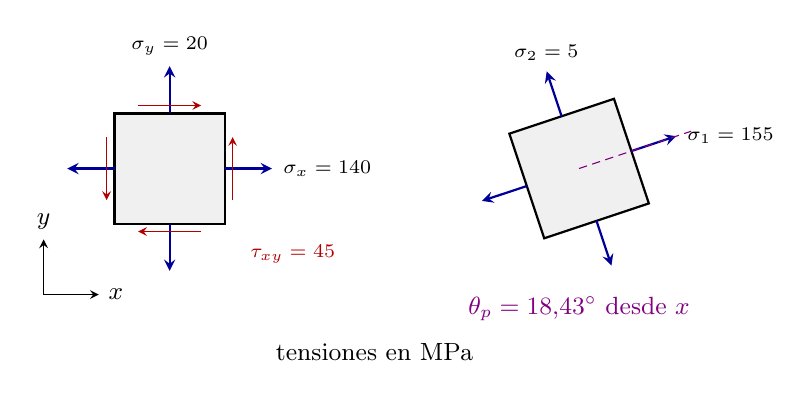
\begin{tikzpicture}
\filldraw[fill=gray!12,thick] (-0.7000,-0.7000) -- (0.7000,-0.7000) -- (0.7000,0.7000) -- (-0.7000,0.7000) -- cycle;
\draw[-stealth,thick,blue!60!black] (0.7000,0.0000) -- (1.3000,0.0000);
\node[font=\scriptsize,anchor=west] at (1.3200,0.0000) {$\sigma_x = 140$};
\draw[-stealth,thick,blue!60!black] (-0.7000,0.0000) -- (-1.3000,0.0000);
\draw[-stealth,thick,blue!60!black] (0.0000,0.7000) -- (0.0000,1.3000);
\node[font=\scriptsize,anchor=south] at (0.0000,1.3200) {$\sigma_y = 20$};
\draw[-stealth,thick,blue!60!black] (0.0000,-0.7000) -- (0.0000,-1.3000);
\draw[-stealth,red!70!black] (0.8000,-0.4000) -- (0.8000,0.4000);
\draw[-stealth,red!70!black] (-0.8000,0.4000) -- (-0.8000,-0.4000);
\draw[-stealth,red!70!black] (-0.4000,0.8000) -- (0.4000,0.8000);
\draw[-stealth,red!70!black] (0.4000,-0.8000) -- (-0.4000,-0.8000);
\node[font=\scriptsize,red!70!black,anchor=north west] at (0.9000,-0.8500) {$\tau_{xy} = 45$};
\filldraw[fill=gray!12,thick] (4.7573,-0.8854) -- (6.0854,-0.4427) -- (5.6427,0.8854) -- (4.3146,0.4427) -- cycle;
\draw[-stealth,thick,blue!60!black] (5.8641,0.2214) -- (6.4333,0.4111);
\node[font=\scriptsize,anchor=west] at (6.4523,0.4174) {$\sigma_1 = 155$};
\draw[-stealth,thick,blue!60!black] (4.5359,-0.2214) -- (3.9667,-0.4111);
\draw[-stealth,thick,blue!60!black] (4.9786,0.6641) -- (4.7889,1.2333);
\node[font=\scriptsize,anchor=south] at (4.7826,1.2523) {$\sigma_2 = 5$};
\draw[-stealth,thick,blue!60!black] (5.4214,-0.6641) -- (5.6111,-1.2333);
\draw[-stealth] (-1.6,-1.6) -- (-0.9,-1.6) node[right,font=\small] {$x$};
\draw[-stealth] (-1.6,-1.6) -- (-1.6,-0.9) node[above,font=\small] {$y$};
\draw[densely dashed,violet] (5.2,0) -- (6.6230,0.4743);
\node[font=\small,violet,anchor=north] at (5.2,-1.5) {$\theta_p = 18{,}43^\circ$ desde $x$};
\node[font=\small,anchor=north] at (2.6,-2.1) {tensiones en MPa};
\end{tikzpicture}}%
\count0=\ht0
\advance\count0 by \dp0
\count2=\wd0
\count4=\dimexpr\textheight/100*38\relax
\count6=\linewidth
\ifnum\count0<1
\count0=1
\fi
\ifnum\count2<1
\count2=1
\fi
\divide\count0 by 4096
\divide\count2 by 4096
\divide\count4 by 4096
\divide\count6 by 4096
\ifnum\count0<1
\count0=1
\fi
\ifnum\count2<1
\count2=1
\fi
\ifnum\count4<1
\count4=1
\fi
\ifnum\count6<1
\count6=1
\fi
\count8=\count2
\ifnum\count0>\count4
\count8=\numexpr\count2*\count4/\count0\relax
\fi
\ifnum\count8>\count6
\resizebox{\linewidth}{!}{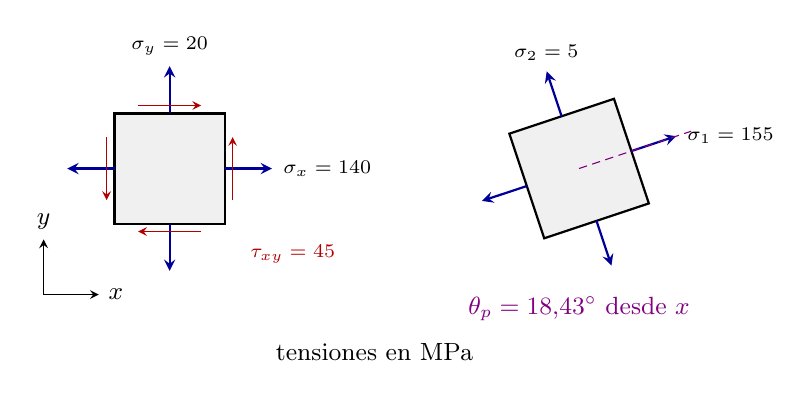
\begin{tikzpicture}
\filldraw[fill=gray!12,thick] (-0.7000,-0.7000) -- (0.7000,-0.7000) -- (0.7000,0.7000) -- (-0.7000,0.7000) -- cycle;
\draw[-stealth,thick,blue!60!black] (0.7000,0.0000) -- (1.3000,0.0000);
\node[font=\scriptsize,anchor=west] at (1.3200,0.0000) {$\sigma_x = 140$};
\draw[-stealth,thick,blue!60!black] (-0.7000,0.0000) -- (-1.3000,0.0000);
\draw[-stealth,thick,blue!60!black] (0.0000,0.7000) -- (0.0000,1.3000);
\node[font=\scriptsize,anchor=south] at (0.0000,1.3200) {$\sigma_y = 20$};
\draw[-stealth,thick,blue!60!black] (0.0000,-0.7000) -- (0.0000,-1.3000);
\draw[-stealth,red!70!black] (0.8000,-0.4000) -- (0.8000,0.4000);
\draw[-stealth,red!70!black] (-0.8000,0.4000) -- (-0.8000,-0.4000);
\draw[-stealth,red!70!black] (-0.4000,0.8000) -- (0.4000,0.8000);
\draw[-stealth,red!70!black] (0.4000,-0.8000) -- (-0.4000,-0.8000);
\node[font=\scriptsize,red!70!black,anchor=north west] at (0.9000,-0.8500) {$\tau_{xy} = 45$};
\filldraw[fill=gray!12,thick] (4.7573,-0.8854) -- (6.0854,-0.4427) -- (5.6427,0.8854) -- (4.3146,0.4427) -- cycle;
\draw[-stealth,thick,blue!60!black] (5.8641,0.2214) -- (6.4333,0.4111);
\node[font=\scriptsize,anchor=west] at (6.4523,0.4174) {$\sigma_1 = 155$};
\draw[-stealth,thick,blue!60!black] (4.5359,-0.2214) -- (3.9667,-0.4111);
\draw[-stealth,thick,blue!60!black] (4.9786,0.6641) -- (4.7889,1.2333);
\node[font=\scriptsize,anchor=south] at (4.7826,1.2523) {$\sigma_2 = 5$};
\draw[-stealth,thick,blue!60!black] (5.4214,-0.6641) -- (5.6111,-1.2333);
\draw[-stealth] (-1.6,-1.6) -- (-0.9,-1.6) node[right,font=\small] {$x$};
\draw[-stealth] (-1.6,-1.6) -- (-1.6,-0.9) node[above,font=\small] {$y$};
\draw[densely dashed,violet] (5.2,0) -- (6.6230,0.4743);
\node[font=\small,violet,anchor=north] at (5.2,-1.5) {$\theta_p = 18{,}43^\circ$ desde $x$};
\node[font=\small,anchor=north] at (2.6,-2.1) {tensiones en MPa};
\end{tikzpicture}}%
\else
\ifnum\count0>\count4
\resizebox{!}{\dimexpr\textheight/100*38\relax}{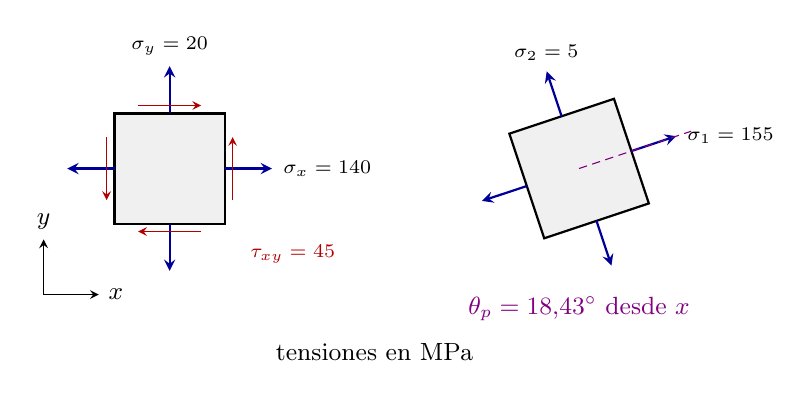
\begin{tikzpicture}
\filldraw[fill=gray!12,thick] (-0.7000,-0.7000) -- (0.7000,-0.7000) -- (0.7000,0.7000) -- (-0.7000,0.7000) -- cycle;
\draw[-stealth,thick,blue!60!black] (0.7000,0.0000) -- (1.3000,0.0000);
\node[font=\scriptsize,anchor=west] at (1.3200,0.0000) {$\sigma_x = 140$};
\draw[-stealth,thick,blue!60!black] (-0.7000,0.0000) -- (-1.3000,0.0000);
\draw[-stealth,thick,blue!60!black] (0.0000,0.7000) -- (0.0000,1.3000);
\node[font=\scriptsize,anchor=south] at (0.0000,1.3200) {$\sigma_y = 20$};
\draw[-stealth,thick,blue!60!black] (0.0000,-0.7000) -- (0.0000,-1.3000);
\draw[-stealth,red!70!black] (0.8000,-0.4000) -- (0.8000,0.4000);
\draw[-stealth,red!70!black] (-0.8000,0.4000) -- (-0.8000,-0.4000);
\draw[-stealth,red!70!black] (-0.4000,0.8000) -- (0.4000,0.8000);
\draw[-stealth,red!70!black] (0.4000,-0.8000) -- (-0.4000,-0.8000);
\node[font=\scriptsize,red!70!black,anchor=north west] at (0.9000,-0.8500) {$\tau_{xy} = 45$};
\filldraw[fill=gray!12,thick] (4.7573,-0.8854) -- (6.0854,-0.4427) -- (5.6427,0.8854) -- (4.3146,0.4427) -- cycle;
\draw[-stealth,thick,blue!60!black] (5.8641,0.2214) -- (6.4333,0.4111);
\node[font=\scriptsize,anchor=west] at (6.4523,0.4174) {$\sigma_1 = 155$};
\draw[-stealth,thick,blue!60!black] (4.5359,-0.2214) -- (3.9667,-0.4111);
\draw[-stealth,thick,blue!60!black] (4.9786,0.6641) -- (4.7889,1.2333);
\node[font=\scriptsize,anchor=south] at (4.7826,1.2523) {$\sigma_2 = 5$};
\draw[-stealth,thick,blue!60!black] (5.4214,-0.6641) -- (5.6111,-1.2333);
\draw[-stealth] (-1.6,-1.6) -- (-0.9,-1.6) node[right,font=\small] {$x$};
\draw[-stealth] (-1.6,-1.6) -- (-1.6,-0.9) node[above,font=\small] {$y$};
\draw[densely dashed,violet] (5.2,0) -- (6.6230,0.4743);
\node[font=\small,violet,anchor=north] at (5.2,-1.5) {$\theta_p = 18{,}43^\circ$ desde $x$};
\node[font=\small,anchor=north] at (2.6,-2.1) {tensiones en MPa};
\end{tikzpicture}}%
\else
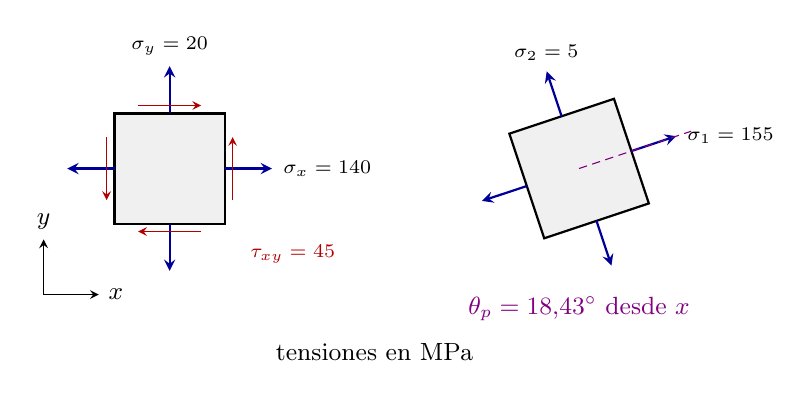
\begin{tikzpicture}
\filldraw[fill=gray!12,thick] (-0.7000,-0.7000) -- (0.7000,-0.7000) -- (0.7000,0.7000) -- (-0.7000,0.7000) -- cycle;
\draw[-stealth,thick,blue!60!black] (0.7000,0.0000) -- (1.3000,0.0000);
\node[font=\scriptsize,anchor=west] at (1.3200,0.0000) {$\sigma_x = 140$};
\draw[-stealth,thick,blue!60!black] (-0.7000,0.0000) -- (-1.3000,0.0000);
\draw[-stealth,thick,blue!60!black] (0.0000,0.7000) -- (0.0000,1.3000);
\node[font=\scriptsize,anchor=south] at (0.0000,1.3200) {$\sigma_y = 20$};
\draw[-stealth,thick,blue!60!black] (0.0000,-0.7000) -- (0.0000,-1.3000);
\draw[-stealth,red!70!black] (0.8000,-0.4000) -- (0.8000,0.4000);
\draw[-stealth,red!70!black] (-0.8000,0.4000) -- (-0.8000,-0.4000);
\draw[-stealth,red!70!black] (-0.4000,0.8000) -- (0.4000,0.8000);
\draw[-stealth,red!70!black] (0.4000,-0.8000) -- (-0.4000,-0.8000);
\node[font=\scriptsize,red!70!black,anchor=north west] at (0.9000,-0.8500) {$\tau_{xy} = 45$};
\filldraw[fill=gray!12,thick] (4.7573,-0.8854) -- (6.0854,-0.4427) -- (5.6427,0.8854) -- (4.3146,0.4427) -- cycle;
\draw[-stealth,thick,blue!60!black] (5.8641,0.2214) -- (6.4333,0.4111);
\node[font=\scriptsize,anchor=west] at (6.4523,0.4174) {$\sigma_1 = 155$};
\draw[-stealth,thick,blue!60!black] (4.5359,-0.2214) -- (3.9667,-0.4111);
\draw[-stealth,thick,blue!60!black] (4.9786,0.6641) -- (4.7889,1.2333);
\node[font=\scriptsize,anchor=south] at (4.7826,1.2523) {$\sigma_2 = 5$};
\draw[-stealth,thick,blue!60!black] (5.4214,-0.6641) -- (5.6111,-1.2333);
\draw[-stealth] (-1.6,-1.6) -- (-0.9,-1.6) node[right,font=\small] {$x$};
\draw[-stealth] (-1.6,-1.6) -- (-1.6,-0.9) node[above,font=\small] {$y$};
\draw[densely dashed,violet] (5.2,0) -- (6.6230,0.4743);
\node[font=\small,violet,anchor=north] at (5.2,-1.5) {$\theta_p = 18{,}43^\circ$ desde $x$};
\node[font=\small,anchor=north] at (2.6,-2.1) {tensiones en MPa};
\end{tikzpicture}%
\fi
\fi
\endgroup
\par\nopagebreak
\studiumcaption{fig:e2-c08-w_rotacion_panel-elemento}{Estado tensional inicial y elemento principal con los resultados del cálculo. Figura reservada a la solución.}
\end{minipage}\par\medskip

\par\medskip\noindent\begin{minipage}{\linewidth}
\centering
\begingroup
\setbox0=\hbox{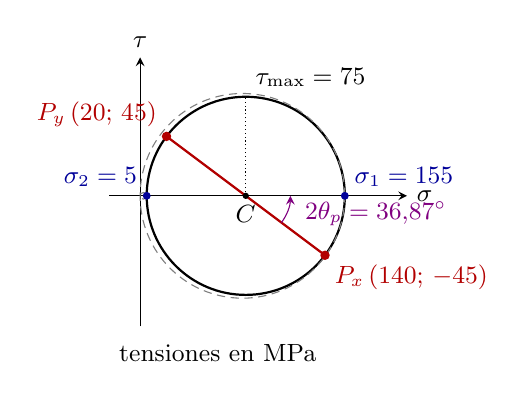
\begin{tikzpicture}
\draw[-stealth] (-0.3900,0) -- (3.3900,0) node[right,font=\small] {$\sigma$};
\draw[-stealth] (0,-1.6581) -- (0,1.7581) node[above,font=\small] {$\tau$};
% studium:circle centre=80.0 radius=75.0 scale=0.016774193548387096
\draw[thick] (1.3419,0) circle (1.2581);
% studium:circle centre=77.5 radius=77.5 scale=0.016774193548387096
\draw[densely dashed,gray] (1.3000,0) circle (1.3000);
% studium:circle centre=2.5 radius=2.5 scale=0.016774193548387096
\draw[densely dashed,gray] (0.0419,0) circle (0.0419);
\draw[red!70!black,thick] (2.3484,-0.7548) -- (0.3355,0.7548);
% studium:mohrpoint Px sigma=140.0 tau=-45.0 scale=0.016774193548387096
\fill[red!70!black] (2.3484,-0.7548) circle (0.06) node[anchor=north west,font=\small] {$P_x\,(140;\,-45)$};
% studium:mohrpoint Py sigma=20.0 tau=45.0 scale=0.016774193548387096
\fill[red!70!black] (0.3355,0.7548) circle (0.06) node[anchor=south east,font=\small] {$P_y\,(20;\,45)$};
\fill (1.3419,0) circle (0.04) node[below,font=\small] {$C$};
\fill[blue!60!black] (2.6000,0) circle (0.05) node[anchor=south west,font=\small,blue!60!black] {$\sigma_1 = 155$};
\fill[blue!60!black] (0.0839,0) circle (0.05) node[anchor=south east,font=\small,blue!60!black] {$\sigma_2 = 5$};
\draw[densely dotted] (1.3419,0) -- (1.3419,1.2581) node[above right,font=\small] {$\tau_{\max} = 75$};
\draw[-stealth,violet] (1.7948,-0.3397) arc (-36.870:0:0.5661);
\node[font=\small,violet,anchor=west] at (1.9710,-0.2265) {$2\theta_p = 36{,}87^\circ$};
\node[font=\small,anchor=north west] at (-0.3900,-1.7581) {tensiones en MPa};
\end{tikzpicture}}%
\count0=\ht0
\advance\count0 by \dp0
\count2=\wd0
\count4=\dimexpr\textheight/100*38\relax
\count6=\linewidth
\ifnum\count0<1
\count0=1
\fi
\ifnum\count2<1
\count2=1
\fi
\divide\count0 by 4096
\divide\count2 by 4096
\divide\count4 by 4096
\divide\count6 by 4096
\ifnum\count0<1
\count0=1
\fi
\ifnum\count2<1
\count2=1
\fi
\ifnum\count4<1
\count4=1
\fi
\ifnum\count6<1
\count6=1
\fi
\count8=\count2
\ifnum\count0>\count4
\count8=\numexpr\count2*\count4/\count0\relax
\fi
\ifnum\count8>\count6
\resizebox{\linewidth}{!}{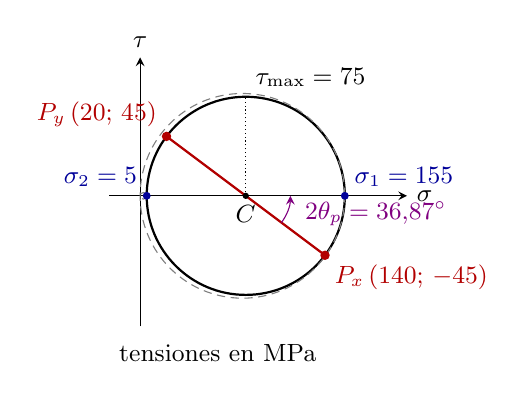
\begin{tikzpicture}
\draw[-stealth] (-0.3900,0) -- (3.3900,0) node[right,font=\small] {$\sigma$};
\draw[-stealth] (0,-1.6581) -- (0,1.7581) node[above,font=\small] {$\tau$};
% studium:circle centre=80.0 radius=75.0 scale=0.016774193548387096
\draw[thick] (1.3419,0) circle (1.2581);
% studium:circle centre=77.5 radius=77.5 scale=0.016774193548387096
\draw[densely dashed,gray] (1.3000,0) circle (1.3000);
% studium:circle centre=2.5 radius=2.5 scale=0.016774193548387096
\draw[densely dashed,gray] (0.0419,0) circle (0.0419);
\draw[red!70!black,thick] (2.3484,-0.7548) -- (0.3355,0.7548);
% studium:mohrpoint Px sigma=140.0 tau=-45.0 scale=0.016774193548387096
\fill[red!70!black] (2.3484,-0.7548) circle (0.06) node[anchor=north west,font=\small] {$P_x\,(140;\,-45)$};
% studium:mohrpoint Py sigma=20.0 tau=45.0 scale=0.016774193548387096
\fill[red!70!black] (0.3355,0.7548) circle (0.06) node[anchor=south east,font=\small] {$P_y\,(20;\,45)$};
\fill (1.3419,0) circle (0.04) node[below,font=\small] {$C$};
\fill[blue!60!black] (2.6000,0) circle (0.05) node[anchor=south west,font=\small,blue!60!black] {$\sigma_1 = 155$};
\fill[blue!60!black] (0.0839,0) circle (0.05) node[anchor=south east,font=\small,blue!60!black] {$\sigma_2 = 5$};
\draw[densely dotted] (1.3419,0) -- (1.3419,1.2581) node[above right,font=\small] {$\tau_{\max} = 75$};
\draw[-stealth,violet] (1.7948,-0.3397) arc (-36.870:0:0.5661);
\node[font=\small,violet,anchor=west] at (1.9710,-0.2265) {$2\theta_p = 36{,}87^\circ$};
\node[font=\small,anchor=north west] at (-0.3900,-1.7581) {tensiones en MPa};
\end{tikzpicture}}%
\else
\ifnum\count0>\count4
\resizebox{!}{\dimexpr\textheight/100*38\relax}{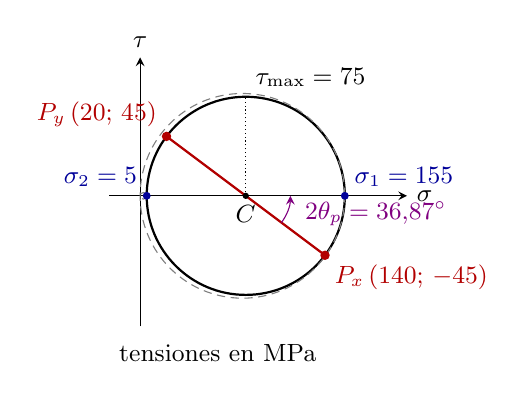
\begin{tikzpicture}
\draw[-stealth] (-0.3900,0) -- (3.3900,0) node[right,font=\small] {$\sigma$};
\draw[-stealth] (0,-1.6581) -- (0,1.7581) node[above,font=\small] {$\tau$};
% studium:circle centre=80.0 radius=75.0 scale=0.016774193548387096
\draw[thick] (1.3419,0) circle (1.2581);
% studium:circle centre=77.5 radius=77.5 scale=0.016774193548387096
\draw[densely dashed,gray] (1.3000,0) circle (1.3000);
% studium:circle centre=2.5 radius=2.5 scale=0.016774193548387096
\draw[densely dashed,gray] (0.0419,0) circle (0.0419);
\draw[red!70!black,thick] (2.3484,-0.7548) -- (0.3355,0.7548);
% studium:mohrpoint Px sigma=140.0 tau=-45.0 scale=0.016774193548387096
\fill[red!70!black] (2.3484,-0.7548) circle (0.06) node[anchor=north west,font=\small] {$P_x\,(140;\,-45)$};
% studium:mohrpoint Py sigma=20.0 tau=45.0 scale=0.016774193548387096
\fill[red!70!black] (0.3355,0.7548) circle (0.06) node[anchor=south east,font=\small] {$P_y\,(20;\,45)$};
\fill (1.3419,0) circle (0.04) node[below,font=\small] {$C$};
\fill[blue!60!black] (2.6000,0) circle (0.05) node[anchor=south west,font=\small,blue!60!black] {$\sigma_1 = 155$};
\fill[blue!60!black] (0.0839,0) circle (0.05) node[anchor=south east,font=\small,blue!60!black] {$\sigma_2 = 5$};
\draw[densely dotted] (1.3419,0) -- (1.3419,1.2581) node[above right,font=\small] {$\tau_{\max} = 75$};
\draw[-stealth,violet] (1.7948,-0.3397) arc (-36.870:0:0.5661);
\node[font=\small,violet,anchor=west] at (1.9710,-0.2265) {$2\theta_p = 36{,}87^\circ$};
\node[font=\small,anchor=north west] at (-0.3900,-1.7581) {tensiones en MPa};
\end{tikzpicture}}%
\else
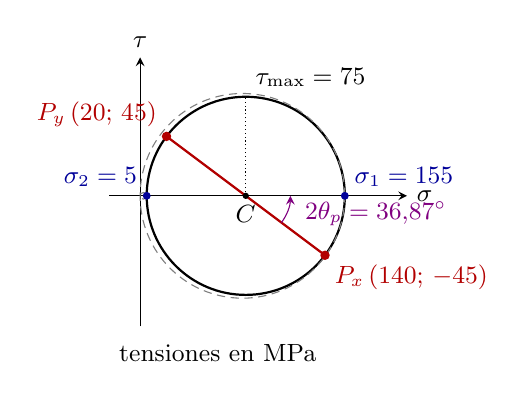
\begin{tikzpicture}
\draw[-stealth] (-0.3900,0) -- (3.3900,0) node[right,font=\small] {$\sigma$};
\draw[-stealth] (0,-1.6581) -- (0,1.7581) node[above,font=\small] {$\tau$};
% studium:circle centre=80.0 radius=75.0 scale=0.016774193548387096
\draw[thick] (1.3419,0) circle (1.2581);
% studium:circle centre=77.5 radius=77.5 scale=0.016774193548387096
\draw[densely dashed,gray] (1.3000,0) circle (1.3000);
% studium:circle centre=2.5 radius=2.5 scale=0.016774193548387096
\draw[densely dashed,gray] (0.0419,0) circle (0.0419);
\draw[red!70!black,thick] (2.3484,-0.7548) -- (0.3355,0.7548);
% studium:mohrpoint Px sigma=140.0 tau=-45.0 scale=0.016774193548387096
\fill[red!70!black] (2.3484,-0.7548) circle (0.06) node[anchor=north west,font=\small] {$P_x\,(140;\,-45)$};
% studium:mohrpoint Py sigma=20.0 tau=45.0 scale=0.016774193548387096
\fill[red!70!black] (0.3355,0.7548) circle (0.06) node[anchor=south east,font=\small] {$P_y\,(20;\,45)$};
\fill (1.3419,0) circle (0.04) node[below,font=\small] {$C$};
\fill[blue!60!black] (2.6000,0) circle (0.05) node[anchor=south west,font=\small,blue!60!black] {$\sigma_1 = 155$};
\fill[blue!60!black] (0.0839,0) circle (0.05) node[anchor=south east,font=\small,blue!60!black] {$\sigma_2 = 5$};
\draw[densely dotted] (1.3419,0) -- (1.3419,1.2581) node[above right,font=\small] {$\tau_{\max} = 75$};
\draw[-stealth,violet] (1.7948,-0.3397) arc (-36.870:0:0.5661);
\node[font=\small,violet,anchor=west] at (1.9710,-0.2265) {$2\theta_p = 36{,}87^\circ$};
\node[font=\small,anchor=north west] at (-0.3900,-1.7581) {tensiones en MPa};
\end{tikzpicture}%
\fi
\fi
\endgroup
\par\nopagebreak
\studiumcaption{fig:e2-c08-w_rotacion_panel-mohr}{Círculo de Mohr con los puntos de las caras, tensiones principales y referencia del ángulo. Figura reservada a la solución.}
\end{minipage}\par\medskip

\textbf{Resultado e interpretación.}\[\fitmath{\begin{aligned}\sigma_{1,\mathrm{plano}} &\approx 155\,\mathrm{MPa},\quad \sigma_{2,\mathrm{plano}} \approx 5\,\mathrm{MPa}\\\sigma_{VM} &\approx 152{,}6\,\mathrm{MPa},\quad \sigma_{Tresca} \approx 155\,\mathrm{MPa}\\\sigma_{x\prime} \approx 149\,\mathrm{MPa}\end{aligned}}\]

La rotación del sistema de referencia conserva la traza y el determinante del estado plano, aunque cambien sus componentes.

\par\textbf{Comprobación.} Incluye la tercera tensión principal al evaluar Tresca y von Mises. Comprueba los invariantes antes y después de girar los ejes.

\textbf{Límites.}\begin{itemize}\item El motor solo admite cortante xy y la tensión normal z; no modela cortantes xz e yz distintos de cero.
\item El criterio de plastificación es aplicable a materiales metálicos dúctiles e isótropos.
\item Las comprobaciones reproducen el modelo indicado, no su validez constitutiva fuera del régimen elástico.\end{itemize}

\textbf{Errores frecuentes.}\begin{itemize}\item Confundir la máxima cortadura del plano xy con la máxima cortadura absoluta del tensor tridimensional.
\item Olvidar el signo de tau xy al transformar las componentes a otro plano.
\item Aplicar Tresca sin incluir la tercera tensión principal.\end{itemize}

\end{studiumworked}

\chapter{Soluciones del simulacro 2}

\objetivos{Contrasta primero el modelo y después las cifras; aplica la rúbrica del enunciado.}

\Needspace{.3\textheight}

\begin{studiumworked}{PRB-0152}

\section{PRB-0152 · Disminución del diámetro}

\textbf{Enunciado.} Una barra (diámetro 20 mm, $\nu = 0{,}33$) se alarga una deformación axial de $2{,}0\times 10^{-3}$. Calcule la disminución de su diámetro, en milímetros.

\par\medskip\noindent\begin{tabular}{@{}p{.18\linewidth}p{.26\linewidth}p{.48\linewidth}@{}}
\toprule Símbolo & Valor y unidad & Significado\\\midrule
$\nu$ & $0.33$ & coeficiente de Poisson del 7075\\
$\varepsilon_a$ & $0.002$ & deformación axial\\
$d$ & $20\,\mathrm{mm}$ & diámetro\\
\bottomrule\end{tabular}\par\medskip

\textbf{Hipótesis.}\begin{itemize}\item material isótropo lineal
\item deformación transversal uniforme\end{itemize}

\textbf{Modelo y desarrollo.}

Efecto Poisson.\[\fitmath{\Delta d = \nu\,\varepsilon_{a}\,d}\]

\textbf{Procedimiento.}\begin{itemize}\item La deformación transversal es $\varepsilon_t = -\nu\varepsilon_a$.
\item El cambio de diámetro es $\varepsilon_t d$ en valor absoluto.\end{itemize}

\textbf{Cálculo de los pasos.}\begin{enumerate}

\item Disminución del diámetro.

\[\fitmath{0.33 \cdot 0.002 \cdot 20\approx 0.0132\,\mathrm{mm}}\]

\end{enumerate}

\textbf{Resultado e interpretación.}\[\fitmath{\Delta d \approx 0{,}0132\ \mathrm{mm}}\]

La contracción es de $13$ $\mu$m, del orden de una milésima del diámetro: el cambio de sección es despreciable en el cálculo de esfuerzos.

\par\textbf{Comprobación.} Distingue tensión, deformación y desplazamiento. Comprueba el signo de la contracción transversal y la definición de cortadura ingenieril.

\textbf{Límites.}\begin{itemize}\item solo en el tramo elástico\end{itemize}

\textbf{Errores frecuentes.}\begin{itemize}\item olvidar que el diámetro disminuye y no aumenta\end{itemize}

\end{studiumworked}

\Needspace{.3\textheight}

\begin{studiumworked}{PRB-0202}

\section{PRB-0202 · Flexión desviada de un rectángulo}

\textbf{Enunciado.} Una sección rectangular de 60 \ensuremath{\times} 120 mm soporta simultáneamente M\_z = $4\sqrt{3}$ kN·m y M\_y = 4 kN·m. Dibuje la sección y sus ejes centrales, determine las propiedades geométricas y represente las regiones de tracción y compresión y la línea neutra. Obtenga las tensiones extremas.

\par\medskip\noindent\begin{tabular}{@{}p{.18\linewidth}p{.26\linewidth}p{.48\linewidth}@{}}
\toprule Símbolo & Valor y unidad & Significado\\\midrule
$b_{1}$ & $60\,\mathrm{mm}$ & anchura de rectángulo\\
$h_{1}$ & $120\,\mathrm{mm}$ & altura de rectángulo\\
$Mz$ & $6928203.230275509\,\mathrm{N\,mm}$ & esfuerzo aplicado con signo\\
$My$ & $4000000.0\,\mathrm{N\,mm}$ & esfuerzo aplicado con signo\\
\bottomrule\end{tabular}\par\medskip

\par\medskip\noindent\begin{minipage}{\linewidth}
\centering
\begingroup
\setbox0=\hbox{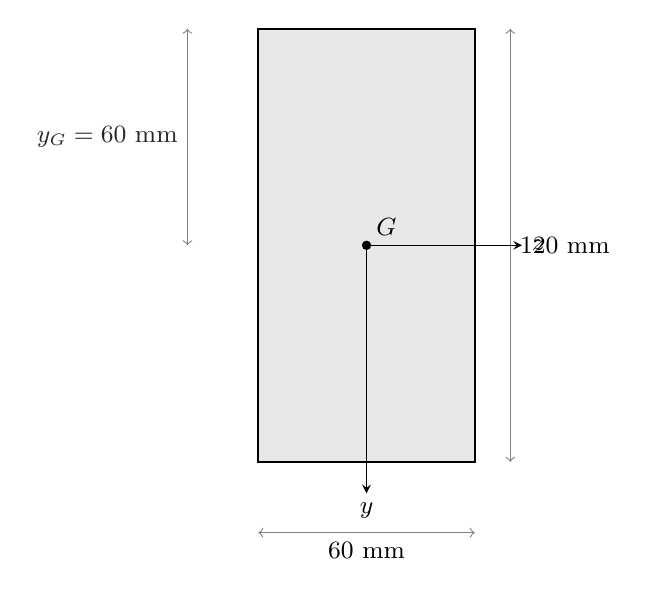
\begin{tikzpicture}
% studium:polygon rectángulo
\filldraw[fill=gray!18,draw=black,thick] (0.0000,0.0000) -- (2.7500,0.0000) -- (2.7500,-5.5000) -- (0.0000,-5.5000) -- cycle;
\draw[<->,gray] (0.0000,-6.4000) -- (2.7500,-6.4000);
\node[font=\small,anchor=north] at (1.3750,-6.4000) {$60$~\mbox{mm}};
\draw[<->,gray] (3.2000,0.0000) -- (3.2000,-5.5000);
\node[font=\small,anchor=west] at (3.2000,-2.7500) {$120$~\mbox{mm}};
% studium:point G z=30 y=60
\fill[black] (1.3750,-2.7500) circle (0.06);
\node[font=\small,anchor=south west] at (1.3750,-2.7500) {$G$};
\draw[-stealth,thin] (1.3750,-2.7500) -- (3.3500,-2.7500) node[right,font=\small] {$z$};
\draw[-stealth,thin] (1.3750,-2.7500) -- (1.3750,-5.9000) node[below,font=\small] {$y$};
\draw[<->,gray] (-0.9000,0.0000) -- (-0.9000,-2.7500);
\node[font=\small,anchor=east,gray!30!black] at (-0.9000,-1.3750) {$y_G = 60$~\mbox{mm}};
\end{tikzpicture}}%
\count0=\ht0
\advance\count0 by \dp0
\count2=\wd0
\count4=\dimexpr\textheight/100*38\relax
\count6=\linewidth
\ifnum\count0<1
\count0=1
\fi
\ifnum\count2<1
\count2=1
\fi
\divide\count0 by 4096
\divide\count2 by 4096
\divide\count4 by 4096
\divide\count6 by 4096
\ifnum\count0<1
\count0=1
\fi
\ifnum\count2<1
\count2=1
\fi
\ifnum\count4<1
\count4=1
\fi
\ifnum\count6<1
\count6=1
\fi
\count8=\count2
\ifnum\count0>\count4
\count8=\numexpr\count2*\count4/\count0\relax
\fi
\ifnum\count8>\count6
\resizebox{\linewidth}{!}{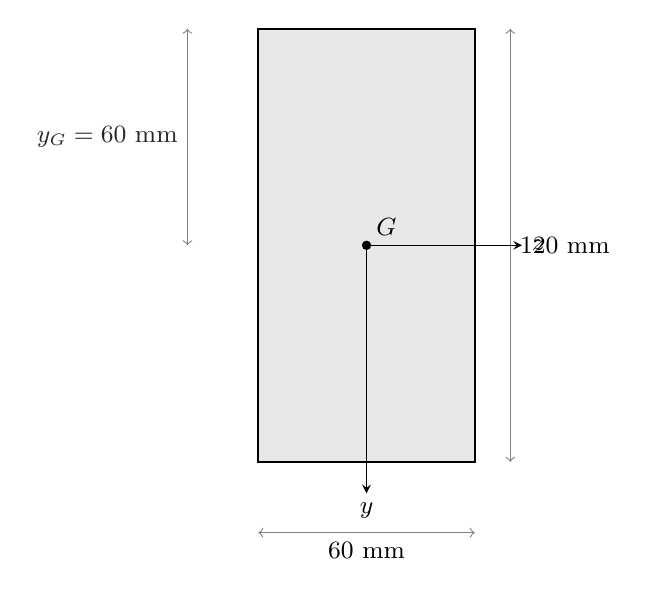
\begin{tikzpicture}
% studium:polygon rectángulo
\filldraw[fill=gray!18,draw=black,thick] (0.0000,0.0000) -- (2.7500,0.0000) -- (2.7500,-5.5000) -- (0.0000,-5.5000) -- cycle;
\draw[<->,gray] (0.0000,-6.4000) -- (2.7500,-6.4000);
\node[font=\small,anchor=north] at (1.3750,-6.4000) {$60$~\mbox{mm}};
\draw[<->,gray] (3.2000,0.0000) -- (3.2000,-5.5000);
\node[font=\small,anchor=west] at (3.2000,-2.7500) {$120$~\mbox{mm}};
% studium:point G z=30 y=60
\fill[black] (1.3750,-2.7500) circle (0.06);
\node[font=\small,anchor=south west] at (1.3750,-2.7500) {$G$};
\draw[-stealth,thin] (1.3750,-2.7500) -- (3.3500,-2.7500) node[right,font=\small] {$z$};
\draw[-stealth,thin] (1.3750,-2.7500) -- (1.3750,-5.9000) node[below,font=\small] {$y$};
\draw[<->,gray] (-0.9000,0.0000) -- (-0.9000,-2.7500);
\node[font=\small,anchor=east,gray!30!black] at (-0.9000,-1.3750) {$y_G = 60$~\mbox{mm}};
\end{tikzpicture}}%
\else
\ifnum\count0>\count4
\resizebox{!}{\dimexpr\textheight/100*38\relax}{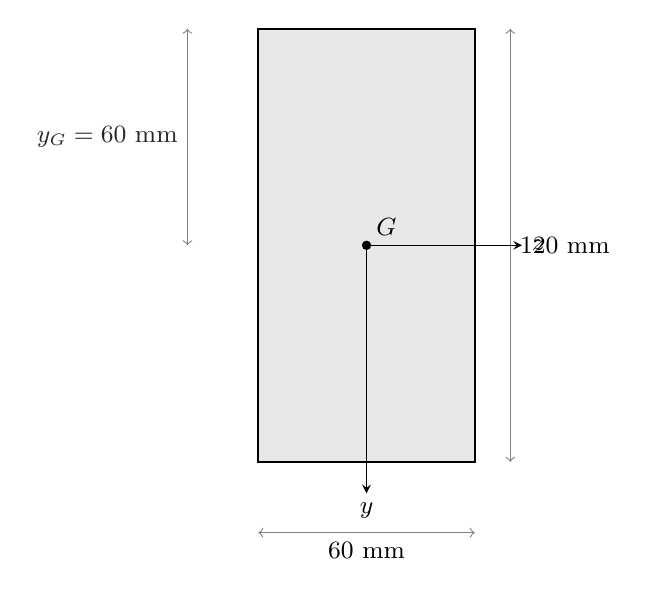
\begin{tikzpicture}
% studium:polygon rectángulo
\filldraw[fill=gray!18,draw=black,thick] (0.0000,0.0000) -- (2.7500,0.0000) -- (2.7500,-5.5000) -- (0.0000,-5.5000) -- cycle;
\draw[<->,gray] (0.0000,-6.4000) -- (2.7500,-6.4000);
\node[font=\small,anchor=north] at (1.3750,-6.4000) {$60$~\mbox{mm}};
\draw[<->,gray] (3.2000,0.0000) -- (3.2000,-5.5000);
\node[font=\small,anchor=west] at (3.2000,-2.7500) {$120$~\mbox{mm}};
% studium:point G z=30 y=60
\fill[black] (1.3750,-2.7500) circle (0.06);
\node[font=\small,anchor=south west] at (1.3750,-2.7500) {$G$};
\draw[-stealth,thin] (1.3750,-2.7500) -- (3.3500,-2.7500) node[right,font=\small] {$z$};
\draw[-stealth,thin] (1.3750,-2.7500) -- (1.3750,-5.9000) node[below,font=\small] {$y$};
\draw[<->,gray] (-0.9000,0.0000) -- (-0.9000,-2.7500);
\node[font=\small,anchor=east,gray!30!black] at (-0.9000,-1.3750) {$y_G = 60$~\mbox{mm}};
\end{tikzpicture}}%
\else
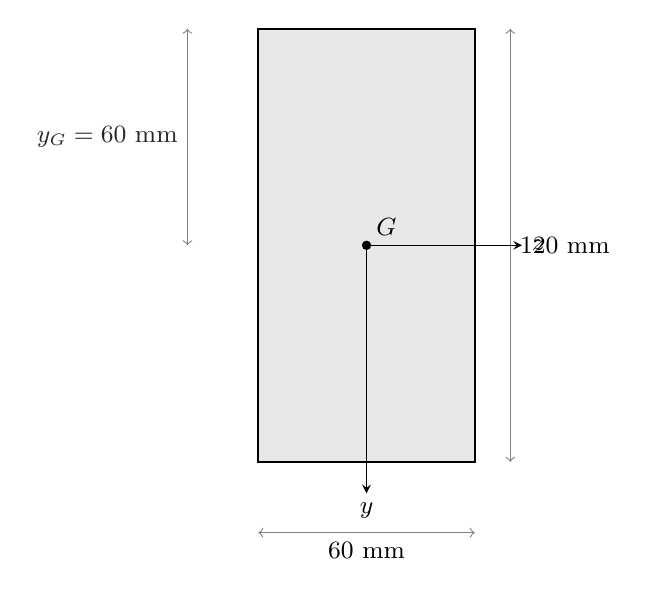
\begin{tikzpicture}
% studium:polygon rectángulo
\filldraw[fill=gray!18,draw=black,thick] (0.0000,0.0000) -- (2.7500,0.0000) -- (2.7500,-5.5000) -- (0.0000,-5.5000) -- cycle;
\draw[<->,gray] (0.0000,-6.4000) -- (2.7500,-6.4000);
\node[font=\small,anchor=north] at (1.3750,-6.4000) {$60$~\mbox{mm}};
\draw[<->,gray] (3.2000,0.0000) -- (3.2000,-5.5000);
\node[font=\small,anchor=west] at (3.2000,-2.7500) {$120$~\mbox{mm}};
% studium:point G z=30 y=60
\fill[black] (1.3750,-2.7500) circle (0.06);
\node[font=\small,anchor=south west] at (1.3750,-2.7500) {$G$};
\draw[-stealth,thin] (1.3750,-2.7500) -- (3.3500,-2.7500) node[right,font=\small] {$z$};
\draw[-stealth,thin] (1.3750,-2.7500) -- (1.3750,-5.9000) node[below,font=\small] {$y$};
\draw[<->,gray] (-0.9000,0.0000) -- (-0.9000,-2.7500);
\node[font=\small,anchor=east,gray!30!black] at (-0.9000,-1.3750) {$y_G = 60$~\mbox{mm}};
\end{tikzpicture}%
\fi
\fi
\endgroup
\par\nopagebreak
\studiumcaption{fig:e2-c04-w_desviada-seccion}{Geometría original de la sección, ejes, centroide y propiedades geométricas.}
\end{minipage}\par\medskip

\textbf{Hipótesis.}\begin{itemize}\item sección prismática y coordenadas y/z declaradas
\item tensiones elásticas lineales cuando se aplican N, M\_y, M\_z
\item cargas y dimensiones expresadas en N y mm\end{itemize}

\textbf{Modelo y desarrollo.}

Momentos geométricos y ley de Navier.\[\fitmath{A = \sum_i A_i,\quad y_G = \frac{\sum_i A_i y_i}{A},\quad I_z = \sum_i (I_{z,i}+A_i d_i^2)}\]

Flexión compuesta en ejes generales.\[\fitmath{\sigma_x = \frac{N}{A}+\frac{(M_z I_y-M_y I_{yz})y+(M_y I_z-M_z I_{yz})z}{I_y I_z-I_{yz}^{2}}}\]

\textbf{Procedimiento.}\begin{itemize}\item La figura establece qué partes pertenecen a la sección, la dirección de y y z y las dimensiones en milímetros.
\item El área total suma las áreas macizas y resta los huecos; los primeros momentos proporcionan las coordenadas del centroide.
\item Calcular I\_z por suma de las inercias propias de las piezas más A\_i por el cuadrado de cada distancia a G (Steiner).
\item El verificador geométrico de Studium contrasta las inercias por otra vía: integración directa sobre los contornos.
\item La tensión normal combina N/A y la flexión alrededor de los ejes centrales; si I\_yz no es cero se conserva en la relación general.
\item Determinar las fibras de tensión extrema evaluando la distribución lineal en los vértices y representar las zonas de compresión y tracción.\end{itemize}

\textbf{Cálculo de los pasos.}\begin{enumerate}

\item Área algebraica de la sección, descontando los huecos.

\[\fitmath{\left(60 - 0\right) \left(120 - 0\right)\approx 7200\,\mathrm{mm^2}}\]

\item Centroide en el eje vertical mediante primeros momentos.

\[\fitmath{\frac{\left(0 + 120\right) \left(60 - 0\right) \left(120 - 0\right)}{2 \left(60 - 0\right) \left(120 - 0\right)}\approx 60\,\mathrm{mm}}\]

\item Momento de inercia I\_z mediante el teorema de Steiner.

Se separa la sustitución en auxiliares numéricos $a_i$, locales a este paso; las unidades corresponden al resultado final.

\[\fitmath{\begin{gathered}a_{1}=\frac{\left(60 - 0\right) \left(120 - 0\right)^{3}}{12}\\a_{2}=\left(\left(-1\right) 60 + \frac{0 + 120}{2}\right)^{2}\\a_{3}=a_{2} \left(60 - 0\right) \left(120 - 0\right)\\a_{4}=a_{1} + a_{3}\\a_{4}\approx 8640000\,\mathrm{mm^4}\end{gathered}}\]

\item Tensión extrema: axil y flexión con el convenio declarado.

\[\fitmath{\frac{250 \sqrt{3}}{9} + \frac{500}{9}\approx 103.66808\,\mathrm{MPa}}\]

\end{enumerate}

\par\medskip\noindent\begin{minipage}{\linewidth}
\centering
\begingroup
\setbox0=\hbox{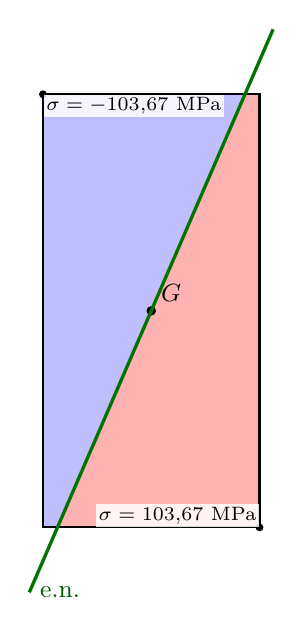
\begin{tikzpicture}
% studium:polygon rectángulo
\filldraw[fill=white,draw=black,thick] (0.0000,0.0000) -- (2.7500,0.0000) -- (2.7500,-5.5000) -- (0.0000,-5.5000) -- cycle;
% studium:zone tension
\fill[red!30] (2.5658,0.0000) -- (2.7500,0.0000) -- (2.7500,-5.5000) -- (0.1842,-5.5000) -- cycle;
% studium:zone compression
\fill[blue!25] (0.0000,0.0000) -- (2.5658,0.0000) -- (0.1842,-5.5000) -- (0.0000,-5.5000) -- cycle;
% studium:polygon rectángulo
\filldraw[fill=none,draw=black,thick] (0.0000,0.0000) -- (2.7500,0.0000) -- (2.7500,-5.5000) -- (0.0000,-5.5000) -- cycle;
% studium:point G z=30 y=60
\fill[black] (1.3750,-2.7500) circle (0.06);
\node[font=\small,anchor=south west] at (1.3750,-2.7500) {$G$};
% studium:neutral-axis z1=63.7749907475931 y1=-18.0 z2=-3.774990747593101 y2=138.0
\draw[very thick,green!45!black] (2.9230,0.8250) -- (-0.1730,-6.3250) node[font=\small,anchor=west,green!35!black] {e.n.};
% studium:value sigma_max z=60 y=120 value=103.67
\fill (2.7500,-5.5000) circle (0.05);
\node[font=\scriptsize,anchor=south east,fill=white,fill opacity=0.85,text opacity=1,inner sep=1pt] at (2.7500,-5.5000) {$\sigma = 103{,}67$~\mbox{MPa}};
% studium:value sigma_min z=0 y=0 value=-103.67
\fill (0.0000,0.0000) circle (0.05);
\node[font=\scriptsize,anchor=north west,fill=white,fill opacity=0.85,text opacity=1,inner sep=1pt] at (0.0000,0.0000) {$\sigma = -103{,}67$~\mbox{MPa}};
\end{tikzpicture}}%
\count0=\ht0
\advance\count0 by \dp0
\count2=\wd0
\count4=\dimexpr\textheight/100*38\relax
\count6=\linewidth
\ifnum\count0<1
\count0=1
\fi
\ifnum\count2<1
\count2=1
\fi
\divide\count0 by 4096
\divide\count2 by 4096
\divide\count4 by 4096
\divide\count6 by 4096
\ifnum\count0<1
\count0=1
\fi
\ifnum\count2<1
\count2=1
\fi
\ifnum\count4<1
\count4=1
\fi
\ifnum\count6<1
\count6=1
\fi
\count8=\count2
\ifnum\count0>\count4
\count8=\numexpr\count2*\count4/\count0\relax
\fi
\ifnum\count8>\count6
\resizebox{\linewidth}{!}{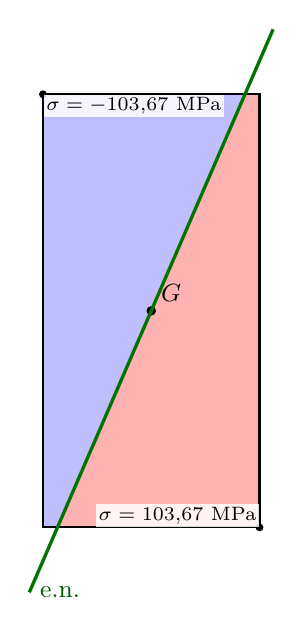
\begin{tikzpicture}
% studium:polygon rectángulo
\filldraw[fill=white,draw=black,thick] (0.0000,0.0000) -- (2.7500,0.0000) -- (2.7500,-5.5000) -- (0.0000,-5.5000) -- cycle;
% studium:zone tension
\fill[red!30] (2.5658,0.0000) -- (2.7500,0.0000) -- (2.7500,-5.5000) -- (0.1842,-5.5000) -- cycle;
% studium:zone compression
\fill[blue!25] (0.0000,0.0000) -- (2.5658,0.0000) -- (0.1842,-5.5000) -- (0.0000,-5.5000) -- cycle;
% studium:polygon rectángulo
\filldraw[fill=none,draw=black,thick] (0.0000,0.0000) -- (2.7500,0.0000) -- (2.7500,-5.5000) -- (0.0000,-5.5000) -- cycle;
% studium:point G z=30 y=60
\fill[black] (1.3750,-2.7500) circle (0.06);
\node[font=\small,anchor=south west] at (1.3750,-2.7500) {$G$};
% studium:neutral-axis z1=63.7749907475931 y1=-18.0 z2=-3.774990747593101 y2=138.0
\draw[very thick,green!45!black] (2.9230,0.8250) -- (-0.1730,-6.3250) node[font=\small,anchor=west,green!35!black] {e.n.};
% studium:value sigma_max z=60 y=120 value=103.67
\fill (2.7500,-5.5000) circle (0.05);
\node[font=\scriptsize,anchor=south east,fill=white,fill opacity=0.85,text opacity=1,inner sep=1pt] at (2.7500,-5.5000) {$\sigma = 103{,}67$~\mbox{MPa}};
% studium:value sigma_min z=0 y=0 value=-103.67
\fill (0.0000,0.0000) circle (0.05);
\node[font=\scriptsize,anchor=north west,fill=white,fill opacity=0.85,text opacity=1,inner sep=1pt] at (0.0000,0.0000) {$\sigma = -103{,}67$~\mbox{MPa}};
\end{tikzpicture}}%
\else
\ifnum\count0>\count4
\resizebox{!}{\dimexpr\textheight/100*38\relax}{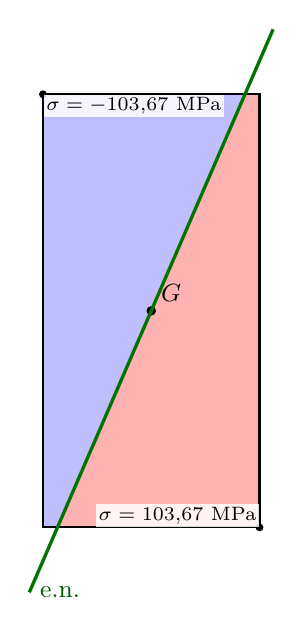
\begin{tikzpicture}
% studium:polygon rectángulo
\filldraw[fill=white,draw=black,thick] (0.0000,0.0000) -- (2.7500,0.0000) -- (2.7500,-5.5000) -- (0.0000,-5.5000) -- cycle;
% studium:zone tension
\fill[red!30] (2.5658,0.0000) -- (2.7500,0.0000) -- (2.7500,-5.5000) -- (0.1842,-5.5000) -- cycle;
% studium:zone compression
\fill[blue!25] (0.0000,0.0000) -- (2.5658,0.0000) -- (0.1842,-5.5000) -- (0.0000,-5.5000) -- cycle;
% studium:polygon rectángulo
\filldraw[fill=none,draw=black,thick] (0.0000,0.0000) -- (2.7500,0.0000) -- (2.7500,-5.5000) -- (0.0000,-5.5000) -- cycle;
% studium:point G z=30 y=60
\fill[black] (1.3750,-2.7500) circle (0.06);
\node[font=\small,anchor=south west] at (1.3750,-2.7500) {$G$};
% studium:neutral-axis z1=63.7749907475931 y1=-18.0 z2=-3.774990747593101 y2=138.0
\draw[very thick,green!45!black] (2.9230,0.8250) -- (-0.1730,-6.3250) node[font=\small,anchor=west,green!35!black] {e.n.};
% studium:value sigma_max z=60 y=120 value=103.67
\fill (2.7500,-5.5000) circle (0.05);
\node[font=\scriptsize,anchor=south east,fill=white,fill opacity=0.85,text opacity=1,inner sep=1pt] at (2.7500,-5.5000) {$\sigma = 103{,}67$~\mbox{MPa}};
% studium:value sigma_min z=0 y=0 value=-103.67
\fill (0.0000,0.0000) circle (0.05);
\node[font=\scriptsize,anchor=north west,fill=white,fill opacity=0.85,text opacity=1,inner sep=1pt] at (0.0000,0.0000) {$\sigma = -103{,}67$~\mbox{MPa}};
\end{tikzpicture}}%
\else
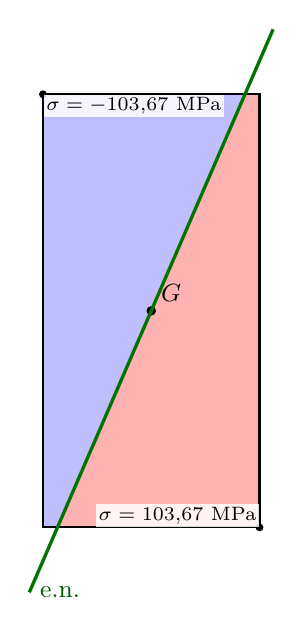
\begin{tikzpicture}
% studium:polygon rectángulo
\filldraw[fill=white,draw=black,thick] (0.0000,0.0000) -- (2.7500,0.0000) -- (2.7500,-5.5000) -- (0.0000,-5.5000) -- cycle;
% studium:zone tension
\fill[red!30] (2.5658,0.0000) -- (2.7500,0.0000) -- (2.7500,-5.5000) -- (0.1842,-5.5000) -- cycle;
% studium:zone compression
\fill[blue!25] (0.0000,0.0000) -- (2.5658,0.0000) -- (0.1842,-5.5000) -- (0.0000,-5.5000) -- cycle;
% studium:polygon rectángulo
\filldraw[fill=none,draw=black,thick] (0.0000,0.0000) -- (2.7500,0.0000) -- (2.7500,-5.5000) -- (0.0000,-5.5000) -- cycle;
% studium:point G z=30 y=60
\fill[black] (1.3750,-2.7500) circle (0.06);
\node[font=\small,anchor=south west] at (1.3750,-2.7500) {$G$};
% studium:neutral-axis z1=63.7749907475931 y1=-18.0 z2=-3.774990747593101 y2=138.0
\draw[very thick,green!45!black] (2.9230,0.8250) -- (-0.1730,-6.3250) node[font=\small,anchor=west,green!35!black] {e.n.};
% studium:value sigma_max z=60 y=120 value=103.67
\fill (2.7500,-5.5000) circle (0.05);
\node[font=\scriptsize,anchor=south east,fill=white,fill opacity=0.85,text opacity=1,inner sep=1pt] at (2.7500,-5.5000) {$\sigma = 103{,}67$~\mbox{MPa}};
% studium:value sigma_min z=0 y=0 value=-103.67
\fill (0.0000,0.0000) circle (0.05);
\node[font=\scriptsize,anchor=north west,fill=white,fill opacity=0.85,text opacity=1,inner sep=1pt] at (0.0000,0.0000) {$\sigma = -103{,}67$~\mbox{MPa}};
\end{tikzpicture}%
\fi
\fi
\endgroup
\par\nopagebreak
\studiumcaption{fig:e2-c04-w_desviada-tension}{Distribución calculada de tensión normal, eje neutro y valores extremos.}
\end{minipage}\par\medskip

\textbf{Resultado e interpretación.}\[\fitmath{\begin{gathered}y_G \approx 60\ \mathrm{mm}\\I_z \approx 8640000\ \mathrm{mm^4}\\\sigma_{\max} \approx 103{,}66808\ \mathrm{MPa}\\\sigma_{\min} \approx -103{,}66808\ \mathrm{MPa}\end{gathered}}\]

La tensión cambia de signo a lo largo de una línea neutra oblicua; en el dibujo deben distinguirse las fibras traccionadas y comprimidas.

\par\textbf{Comprobación.} Fija los ejes centroidales y el signo del axil y del flector. Comprueba la posición del eje neutro y la fibra extrema.

\textbf{Límites.}\begin{itemize}\item no se analizan plastificación, pandeo ni tensiones locales en uniones\end{itemize}

\textbf{Errores frecuentes.}\begin{itemize}\item Eliminar M\_y por ser simétrica la sección.
\item Concluir que el eje neutro tiene que ser horizontal.\end{itemize}

\end{studiumworked}

\Needspace{.3\textheight}

\begin{studiumworked}{PRB-0123}

\section{PRB-0123 · Distancia del centro de cortadura al alma}

\textbf{Enunciado.} Un perfil en C de pared delgada tiene un alma de 100 mm de altura y dos alas de 50 mm de ancho, con un espesor de 2 mm en todas sus paredes (dimensiones de la línea media). Soporta un cortante vertical de 2 kN en el plano del alma. Calcule su inercia, el flujo máximo en el alma, y la distancia del centro de cortadura al alma.

\par\medskip\noindent\begin{tabular}{@{}p{.18\linewidth}p{.26\linewidth}p{.48\linewidth}@{}}
\toprule Símbolo & Valor y unidad & Significado\\\midrule
$h$ & $100\,\mathrm{mm}$ & altura del alma\\
$b$ & $50\,\mathrm{mm}$ & ancho de las alas\\
$t$ & $2\,\mathrm{mm}$ & espesor\\
$C_{y}$ & $2000\,\mathrm{N}$ & cortante\\
\bottomrule\end{tabular}\par\medskip

\textbf{Hipótesis.}\begin{itemize}\item pared delgada
\item se desprecia la inercia propia de las alas
\item cortante en el plano del alma\end{itemize}

\textbf{Modelo y desarrollo.}

Centro de cortadura del perfil en C.\[\fitmath{e_c = \frac{3\,b^{2}}{h + 6b}}\]

\textbf{Procedimiento.}\begin{itemize}\item La inercia es $t h^2 (h + 6b)/12$.
\item El flujo en el eje neutro es $C_y Q_{max}/I_z$ con $Q_{max} = t\,(b h/2 + h^2/8)$.
\item El centro de cortadura está a $3b^2/(h + 6b)$ de la línea media del alma, en el lado opuesto al de las alas.\end{itemize}

\textbf{Cálculo de los pasos.}\begin{enumerate}

\item Inercia del perfil.

\[\fitmath{\frac{2 \cdot 100^{2} \left(100 + 6 \cdot 50\right)}{12}\approx 6.667\times10^{5}\,\mathrm{mm^4}}\]

\item Flujo máximo en el alma.

Se separa la sustitución en auxiliares numéricos $a_i$, locales a este paso; las unidades corresponden al resultado final.

\[\fitmath{\begin{gathered}a_{1}=\frac{100^{2}}{8} + 50 \cdot 100 \cdot \frac{1}{2}\\a_{2}=\frac{2 \cdot 100^{2} \left(100 + 6 \cdot 50\right)}{12}\\a_{3}=\frac{1}{a_{2}}\\a_{4}=2000 \cdot 2 a_{1} a_{3}\\a_{4}\approx 22.5\,\mathrm{N/mm}\end{gathered}}\]

\item Distancia del centro de cortadura al alma.

\[\fitmath{\frac{3 \cdot 50^{2}}{100 + 6 \cdot 50}\approx 18.75\,\mathrm{mm}}\]

\end{enumerate}

\textbf{Resultado e interpretación.}\[\fitmath{I_z \approx 6{,}67\times 10^{5}\ \mathrm{mm}^{4},\quad f_{max} = 22{,}5\ \mathrm{N/mm},\quad e_c = 18{,}75\ \mathrm{mm}}\]

La tensión máxima en el alma es $11{,}25$ MPa. Si la carga se aplica en el alma, a $18{,}75$ mm del centro de cortadura, aparece un torsor de $2000\cdot 18{,}75 = 37{,}5$ N m.

\par\textbf{Comprobación.} Conserva el sentido del recorrido de cada pared y distingue flujo de cortante y tensión. Si la carga no pasa por el centro de cortadura, incluye el torsor adicional.

\textbf{Límites.}\begin{itemize}\item no se incluye el pandeo por cortante del alma\end{itemize}

\textbf{Errores frecuentes.}\begin{itemize}\item medir $e$ desde el centro de gravedad en lugar de desde el alma
\item olvidar que la carga debe pasar por el centro de cortadura\end{itemize}

\end{studiumworked}

\Needspace{.3\textheight}

\begin{studiumworked}{PRB-0225}

\section{PRB-0225 · Giro del extremo}

\textbf{Enunciado.} Una ménsula de 2,5 m soporta una carga vertical de 3 kN en su extremo. Para E = 71,7 GPa e I = 5,0·10\textsuperscript{7} mm$^4$, obtenga el giro del extremo aplicando un momento virtual unidad y compruébelo derivando la energía de flexión respecto a un momento ficticio.

\par\medskip\noindent\begin{tabular}{@{}p{.18\linewidth}p{.26\linewidth}p{.48\linewidth}@{}}
\toprule Símbolo & Valor y unidad & Significado\\\midrule
$L$ & $2500\,\mathrm{mm}$ & longitud de la viga\\
$E$ & $71700\,\mathrm{MPa}$ & módulo de Young\\
$EI$ & $3585000000000\,\mathrm{N\,mm^2}$ & rigidez a flexión\\
\bottomrule\end{tabular}\par\medskip

\par\medskip\noindent\begin{minipage}{\linewidth}
\centering
\begingroup
\setbox0=\hbox{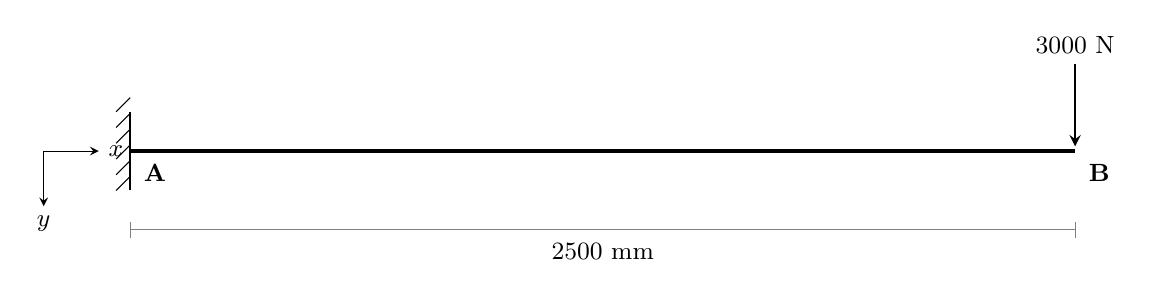
\begin{tikzpicture}
\draw[line width=1.6pt] (0,0.0000) -- (12.0000,0.0000);
% studium:at support A x=0 check=first
\draw[thick] (0.0000,-0.5000) -- (0.0000,0.5000);
\draw (0.0000,-0.3200) -- (-0.1800,-0.5000);
\draw (0.0000,-0.1200) -- (-0.1800,-0.3000);
\draw (0.0000,0.0800) -- (-0.1800,-0.1000);
\draw (0.0000,0.2800) -- (-0.1800,0.1000);
\draw (0.0000,0.4800) -- (-0.1800,0.3000);
\draw (0.0000,0.6800) -- (-0.1800,0.5000);
% studium:at force 0 x=2500 check=tip
\draw[-stealth,thick,black] (12.0000,1.1100) -- (12.0000,0.0600);
\node[font=\small,anchor=south] at (12.0000,1.1100) {$3000$~\mbox{N}};
\node[font=\small\bfseries,anchor=north west] at (0.0500,-0.0500) {A};
\node[font=\small\bfseries,anchor=north west] at (12.0500,-0.0500) {B};
\draw[gray] (0,-1.0000) -- (12.0000,-1.0000);
\draw[gray] (0.0000,-1.1000) -- (0.0000,-0.9000);
\draw[gray] (12.0000,-1.1000) -- (12.0000,-0.9000);
\node[font=\small,anchor=north] at (6.0000,-1.0500) {$2500$~\mbox{mm}};
\draw[-stealth] (-1.1,0.0000) -- (-0.4,0.0000) node[right,font=\small] {$x$};
\draw[-stealth] (-1.1,0.0000) -- (-1.1,-0.7000) node[below,font=\small] {$y$};
\end{tikzpicture}}%
\count0=\ht0
\advance\count0 by \dp0
\count2=\wd0
\count4=\dimexpr\textheight/100*38\relax
\count6=\linewidth
\ifnum\count0<1
\count0=1
\fi
\ifnum\count2<1
\count2=1
\fi
\divide\count0 by 4096
\divide\count2 by 4096
\divide\count4 by 4096
\divide\count6 by 4096
\ifnum\count0<1
\count0=1
\fi
\ifnum\count2<1
\count2=1
\fi
\ifnum\count4<1
\count4=1
\fi
\ifnum\count6<1
\count6=1
\fi
\count8=\count2
\ifnum\count0>\count4
\count8=\numexpr\count2*\count4/\count0\relax
\fi
\ifnum\count8>\count6
\resizebox{\linewidth}{!}{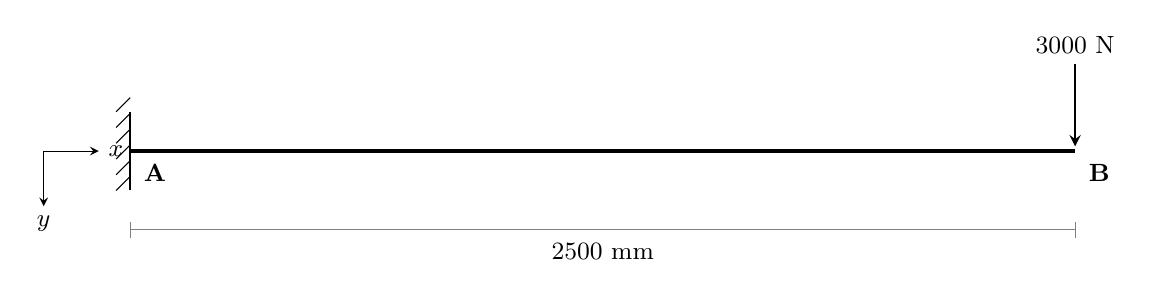
\begin{tikzpicture}
\draw[line width=1.6pt] (0,0.0000) -- (12.0000,0.0000);
% studium:at support A x=0 check=first
\draw[thick] (0.0000,-0.5000) -- (0.0000,0.5000);
\draw (0.0000,-0.3200) -- (-0.1800,-0.5000);
\draw (0.0000,-0.1200) -- (-0.1800,-0.3000);
\draw (0.0000,0.0800) -- (-0.1800,-0.1000);
\draw (0.0000,0.2800) -- (-0.1800,0.1000);
\draw (0.0000,0.4800) -- (-0.1800,0.3000);
\draw (0.0000,0.6800) -- (-0.1800,0.5000);
% studium:at force 0 x=2500 check=tip
\draw[-stealth,thick,black] (12.0000,1.1100) -- (12.0000,0.0600);
\node[font=\small,anchor=south] at (12.0000,1.1100) {$3000$~\mbox{N}};
\node[font=\small\bfseries,anchor=north west] at (0.0500,-0.0500) {A};
\node[font=\small\bfseries,anchor=north west] at (12.0500,-0.0500) {B};
\draw[gray] (0,-1.0000) -- (12.0000,-1.0000);
\draw[gray] (0.0000,-1.1000) -- (0.0000,-0.9000);
\draw[gray] (12.0000,-1.1000) -- (12.0000,-0.9000);
\node[font=\small,anchor=north] at (6.0000,-1.0500) {$2500$~\mbox{mm}};
\draw[-stealth] (-1.1,0.0000) -- (-0.4,0.0000) node[right,font=\small] {$x$};
\draw[-stealth] (-1.1,0.0000) -- (-1.1,-0.7000) node[below,font=\small] {$y$};
\end{tikzpicture}}%
\else
\ifnum\count0>\count4
\resizebox{!}{\dimexpr\textheight/100*38\relax}{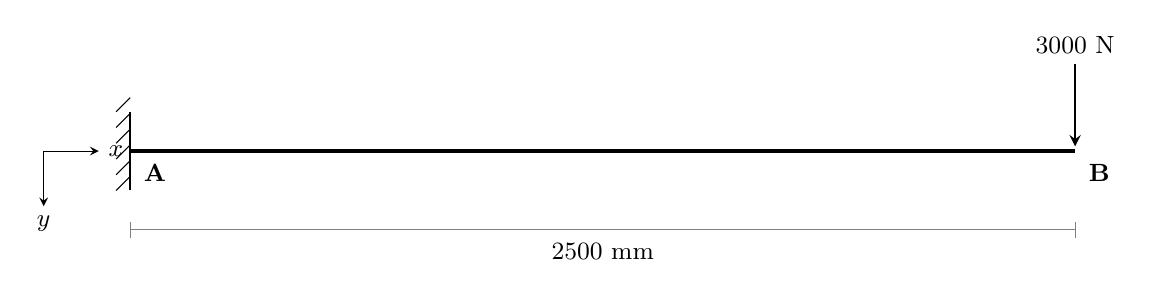
\begin{tikzpicture}
\draw[line width=1.6pt] (0,0.0000) -- (12.0000,0.0000);
% studium:at support A x=0 check=first
\draw[thick] (0.0000,-0.5000) -- (0.0000,0.5000);
\draw (0.0000,-0.3200) -- (-0.1800,-0.5000);
\draw (0.0000,-0.1200) -- (-0.1800,-0.3000);
\draw (0.0000,0.0800) -- (-0.1800,-0.1000);
\draw (0.0000,0.2800) -- (-0.1800,0.1000);
\draw (0.0000,0.4800) -- (-0.1800,0.3000);
\draw (0.0000,0.6800) -- (-0.1800,0.5000);
% studium:at force 0 x=2500 check=tip
\draw[-stealth,thick,black] (12.0000,1.1100) -- (12.0000,0.0600);
\node[font=\small,anchor=south] at (12.0000,1.1100) {$3000$~\mbox{N}};
\node[font=\small\bfseries,anchor=north west] at (0.0500,-0.0500) {A};
\node[font=\small\bfseries,anchor=north west] at (12.0500,-0.0500) {B};
\draw[gray] (0,-1.0000) -- (12.0000,-1.0000);
\draw[gray] (0.0000,-1.1000) -- (0.0000,-0.9000);
\draw[gray] (12.0000,-1.1000) -- (12.0000,-0.9000);
\node[font=\small,anchor=north] at (6.0000,-1.0500) {$2500$~\mbox{mm}};
\draw[-stealth] (-1.1,0.0000) -- (-0.4,0.0000) node[right,font=\small] {$x$};
\draw[-stealth] (-1.1,0.0000) -- (-1.1,-0.7000) node[below,font=\small] {$y$};
\end{tikzpicture}}%
\else
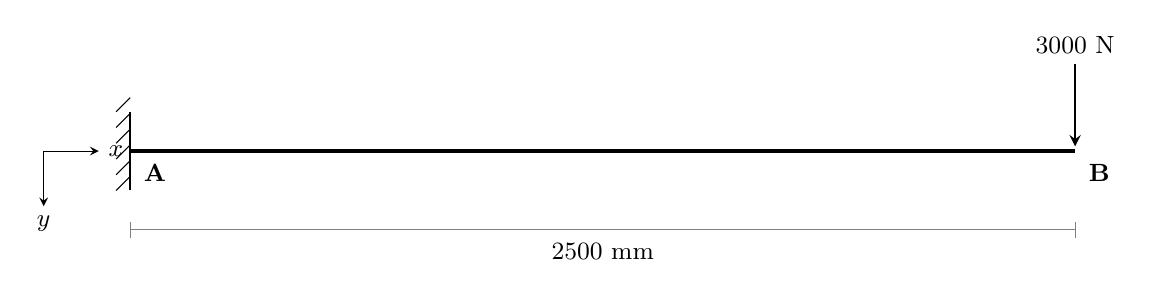
\begin{tikzpicture}
\draw[line width=1.6pt] (0,0.0000) -- (12.0000,0.0000);
% studium:at support A x=0 check=first
\draw[thick] (0.0000,-0.5000) -- (0.0000,0.5000);
\draw (0.0000,-0.3200) -- (-0.1800,-0.5000);
\draw (0.0000,-0.1200) -- (-0.1800,-0.3000);
\draw (0.0000,0.0800) -- (-0.1800,-0.1000);
\draw (0.0000,0.2800) -- (-0.1800,0.1000);
\draw (0.0000,0.4800) -- (-0.1800,0.3000);
\draw (0.0000,0.6800) -- (-0.1800,0.5000);
% studium:at force 0 x=2500 check=tip
\draw[-stealth,thick,black] (12.0000,1.1100) -- (12.0000,0.0600);
\node[font=\small,anchor=south] at (12.0000,1.1100) {$3000$~\mbox{N}};
\node[font=\small\bfseries,anchor=north west] at (0.0500,-0.0500) {A};
\node[font=\small\bfseries,anchor=north west] at (12.0500,-0.0500) {B};
\draw[gray] (0,-1.0000) -- (12.0000,-1.0000);
\draw[gray] (0.0000,-1.1000) -- (0.0000,-0.9000);
\draw[gray] (12.0000,-1.1000) -- (12.0000,-0.9000);
\node[font=\small,anchor=north] at (6.0000,-1.0500) {$2500$~\mbox{mm}};
\draw[-stealth] (-1.1,0.0000) -- (-0.4,0.0000) node[right,font=\small] {$x$};
\draw[-stealth] (-1.1,0.0000) -- (-1.1,-0.7000) node[below,font=\small] {$y$};
\end{tikzpicture}%
\fi
\fi
\endgroup
\par\nopagebreak
\studiumcaption{fig:e2-c07-w_giro_castigliano-enunciado}{Viga real: apoyos, cargas y distancias conocidas, sin reacciones calculadas.}
\end{minipage}\par\medskip

\textbf{Hipótesis.}\begin{itemize}\item respuesta elástica lineal y pequeños desplazamientos
\item teoría de Euler-Bernoulli, sin contribución de energía por cortante
\item módulo E y rigideces EI según enunciado
\item convenio de signos de la ULE\end{itemize}

\textbf{Modelo y desarrollo.}

Trabajo virtual de flexión.\[\fitmath{\delta = \int_{0}^{L}\frac{M(x)\,\overline{M}(x)}{E I(x)}\,\mathrm{d}x}\]

\textbf{Procedimiento.}\begin{itemize}\item Calcular las reacciones del caso real mediante equilibrio y, en su caso, compatibilidad de flechas.
\item Escribir la ley flectora real M(x) en cada intervalo.
\item Introducir un momento virtual unidad en el extremo para hallar su giro.
\item Calcular la ley flectora virtual y sumar las integrales de M por M virtual dividido entre EI para todos los tramos.
\item Verificar el resultado mediante la elástica calculada con constantes de integración y condiciones de apoyo.
\item El flector real es proporcional a la distancia al extremo; para hallar un giro se aplica un MOMENTO virtual de valor unidad, no una fuerza.
\item Contraste por Castigliano: aplicar un momento auxiliar $M_0$ en el extremo y conservarlo como incógnita hasta derivar.
\item Con $x$ medido desde el extremo libre, $M(x)=P x+M_0$ y $U(M_0)=\int_0^L \frac{(P x+M_0)^2}{2EI}\,\mathrm{d}x=\frac{P^2L^3}{6EI}+\frac{PM_0L^2}{2EI}+\frac{M_0^2L}{2EI}$.
\item La derivada energética es $\varphi=\left.\frac{\partial U}{\partial M_0}\right|_{M_0=0}=\frac{PL^2}{2EI}$, con el signo ligado al convenio de giro.\end{itemize}

\textbf{Cálculo de los pasos.}\begin{enumerate}

\item Integral M por M virtual dividida por EI, tramo 1: 0 a 2500 mm.

\[\fitmath{\frac{9375000000}{3585000000000}\approx 0.00261506276\,\mathrm{rad}}\]

\item Verificación por Castigliano con momento ficticio.

\[\fitmath{\varphi=\left.\frac{\partial U}{\partial M_0}\right|_{M_0=0}=\frac{PL^2}{2EI}\approx 0{,}00261506276\,\mathrm{rad}}\]

\item Giro total por suma de tramos.

\[\fitmath{\frac{9375000000}{3585000000000}\approx 0.00261506276\,\mathrm{rad}}\]

\end{enumerate}

\par\medskip\noindent\begin{minipage}{\linewidth}
\centering
\begingroup
\setbox0=\hbox{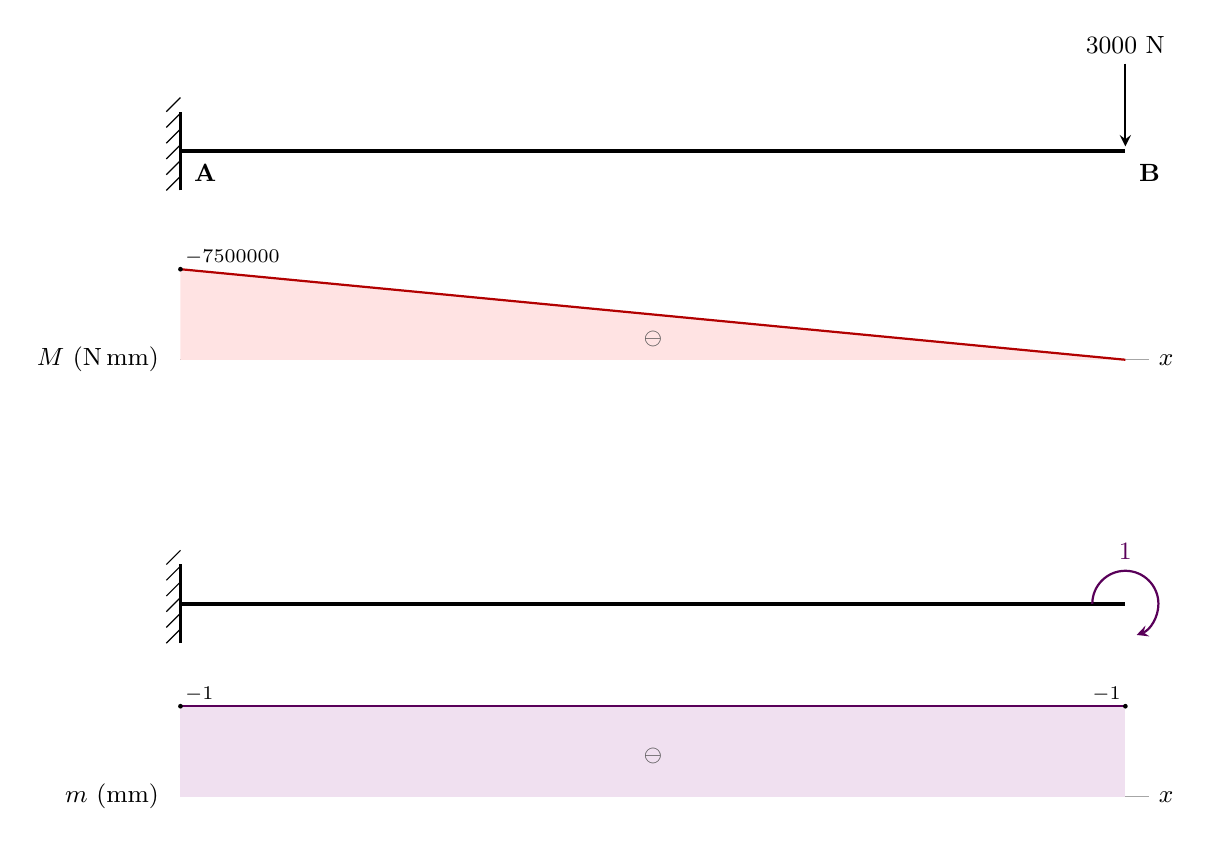
\begin{tikzpicture}
\draw[line width=1.6pt] (0,0.0000) -- (12.0000,0.0000);
% studium:at support A x=0 check=first
\draw[thick] (0.0000,-0.5000) -- (0.0000,0.5000);
\draw (0.0000,-0.3200) -- (-0.1800,-0.5000);
\draw (0.0000,-0.1200) -- (-0.1800,-0.3000);
\draw (0.0000,0.0800) -- (-0.1800,-0.1000);
\draw (0.0000,0.2800) -- (-0.1800,0.1000);
\draw (0.0000,0.4800) -- (-0.1800,0.3000);
\draw (0.0000,0.6800) -- (-0.1800,0.5000);
% studium:at force 0 x=2500 check=tip
\draw[-stealth,thick,black] (12.0000,1.1100) -- (12.0000,0.0600);
\node[font=\small,anchor=south] at (12.0000,1.1100) {$3000$~\mbox{N}};
\node[font=\small\bfseries,anchor=north west] at (0.0500,-0.0500) {A};
\node[font=\small\bfseries,anchor=north west] at (12.0500,-0.0500) {B};
\draw[gray!70] (0,-2.6500) -- (12.3000,-2.6500);
\fill[red!11] (0.0000,-2.6500) -- (0.0000,-1.5000) -- (12.0000,-2.6500) -- (12.0000,-2.6500) -- cycle;
% studium:series M sx=0.0048 sy=1.5333333333333333e-07 x0=0.0 y0=-2.65 sign=-1
\draw[thick,red!70!black] (0.0000,-1.5000) -- (12.0000,-2.6500);
% studium:end M
\node[font=\small,anchor=east] at (-0.15,-2.6500) {$M$ (N\,mm)};
\node[font=\small,anchor=west] at (12.3000,-2.6500) {$x$};
% studium:label M x=0 side=right value=-7500000
\fill (0.0000,-1.5000) circle (0.03);
\node[font=\scriptsize,anchor=south west,inner sep=1.5pt] at (0.0000,-1.5000) {$-7500000$};
\node[font=\footnotesize,gray!60!black] at (6.0000,-2.3912) {$\ominus$};
\draw[line width=1.6pt] (0,-5.7500) -- (12.0000,-5.7500);
% studium:at support A x=0 check=first
\draw[thick] (0.0000,-6.2500) -- (0.0000,-5.2500);
\draw (0.0000,-6.0700) -- (-0.1800,-6.2500);
\draw (0.0000,-5.8700) -- (-0.1800,-6.0500);
\draw (0.0000,-5.6700) -- (-0.1800,-5.8500);
\draw (0.0000,-5.4700) -- (-0.1800,-5.6500);
\draw (0.0000,-5.2700) -- (-0.1800,-5.4500);
\draw (0.0000,-5.0700) -- (-0.1800,-5.2500);
\node[font=\small,anchor=south,violet!70!black] at (12.0000,-5.3100) {$1$};
\draw[-stealth,thick,violet!70!black] (11.5800,-5.7500) arc (180:-70:0.42);
\draw[gray!70] (0,-8.2000) -- (12.3000,-8.2000);
\fill[violet!12] (0.0000,-8.2000) -- (0.0000,-7.0500) -- (12.0000,-7.0500) -- (12.0000,-8.2000) -- cycle;
% studium:series m sx=0.0048 sy=1.15 x0=0.0 y0=-8.2 sign=-1
\draw[thick,violet!70!black] (0.0000,-7.0500) -- (12.0000,-7.0500);
% studium:end m
\node[font=\small,anchor=east] at (-0.15,-8.2000) {$m$ (mm)};
\node[font=\small,anchor=west] at (12.3000,-8.2000) {$x$};
% studium:label m x=0 side=right value=-1
\fill (0.0000,-7.0500) circle (0.03);
\node[font=\scriptsize,anchor=south west,inner sep=1.5pt] at (0.0000,-7.0500) {$-1$};
% studium:label m x=2500 side=left value=-1
\fill (12.0000,-7.0500) circle (0.03);
\node[font=\scriptsize,anchor=south east,inner sep=1.5pt] at (12.0000,-7.0500) {$-1$};
\node[font=\footnotesize,gray!60!black] at (6.0000,-7.6825) {$\ominus$};
\end{tikzpicture}}%
\count0=\ht0
\advance\count0 by \dp0
\count2=\wd0
\count4=\dimexpr\textheight/100*38\relax
\count6=\linewidth
\ifnum\count0<1
\count0=1
\fi
\ifnum\count2<1
\count2=1
\fi
\divide\count0 by 4096
\divide\count2 by 4096
\divide\count4 by 4096
\divide\count6 by 4096
\ifnum\count0<1
\count0=1
\fi
\ifnum\count2<1
\count2=1
\fi
\ifnum\count4<1
\count4=1
\fi
\ifnum\count6<1
\count6=1
\fi
\count8=\count2
\ifnum\count0>\count4
\count8=\numexpr\count2*\count4/\count0\relax
\fi
\ifnum\count8>\count6
\resizebox{\linewidth}{!}{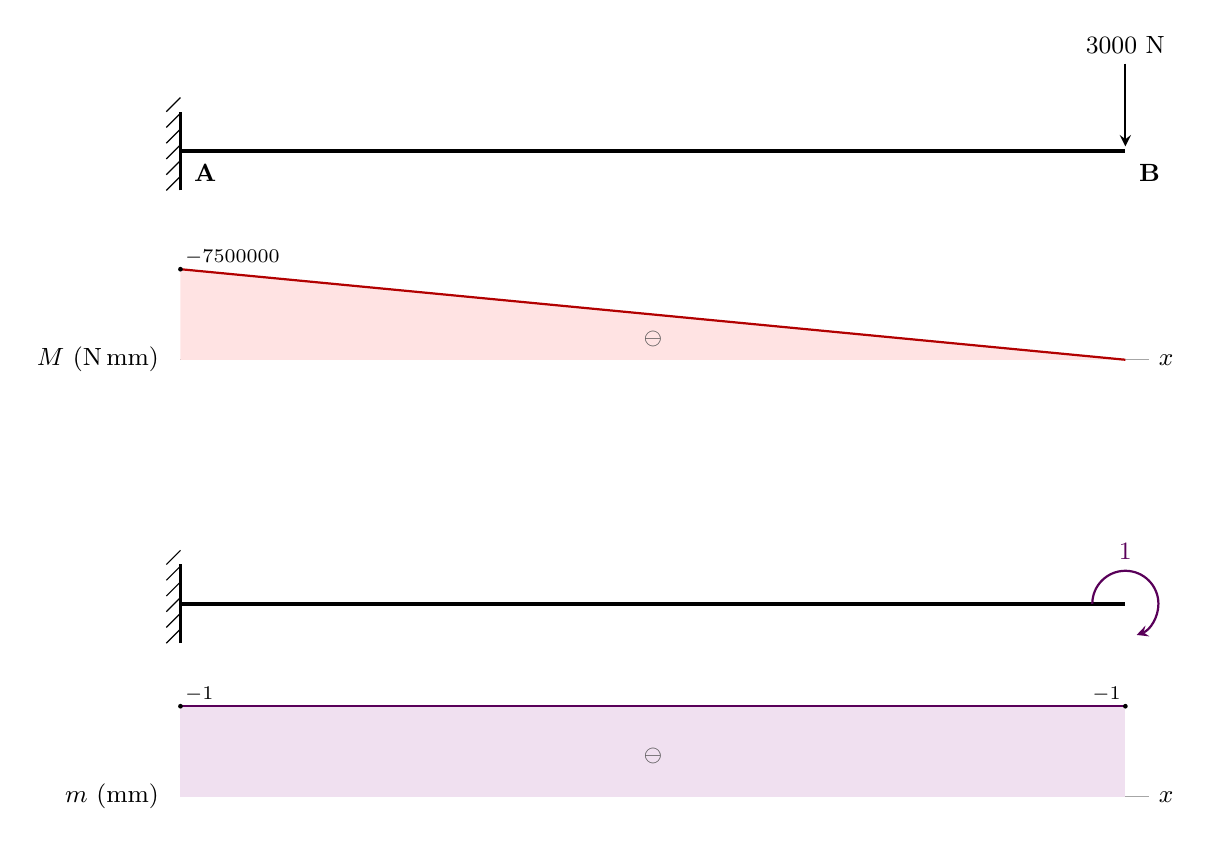
\begin{tikzpicture}
\draw[line width=1.6pt] (0,0.0000) -- (12.0000,0.0000);
% studium:at support A x=0 check=first
\draw[thick] (0.0000,-0.5000) -- (0.0000,0.5000);
\draw (0.0000,-0.3200) -- (-0.1800,-0.5000);
\draw (0.0000,-0.1200) -- (-0.1800,-0.3000);
\draw (0.0000,0.0800) -- (-0.1800,-0.1000);
\draw (0.0000,0.2800) -- (-0.1800,0.1000);
\draw (0.0000,0.4800) -- (-0.1800,0.3000);
\draw (0.0000,0.6800) -- (-0.1800,0.5000);
% studium:at force 0 x=2500 check=tip
\draw[-stealth,thick,black] (12.0000,1.1100) -- (12.0000,0.0600);
\node[font=\small,anchor=south] at (12.0000,1.1100) {$3000$~\mbox{N}};
\node[font=\small\bfseries,anchor=north west] at (0.0500,-0.0500) {A};
\node[font=\small\bfseries,anchor=north west] at (12.0500,-0.0500) {B};
\draw[gray!70] (0,-2.6500) -- (12.3000,-2.6500);
\fill[red!11] (0.0000,-2.6500) -- (0.0000,-1.5000) -- (12.0000,-2.6500) -- (12.0000,-2.6500) -- cycle;
% studium:series M sx=0.0048 sy=1.5333333333333333e-07 x0=0.0 y0=-2.65 sign=-1
\draw[thick,red!70!black] (0.0000,-1.5000) -- (12.0000,-2.6500);
% studium:end M
\node[font=\small,anchor=east] at (-0.15,-2.6500) {$M$ (N\,mm)};
\node[font=\small,anchor=west] at (12.3000,-2.6500) {$x$};
% studium:label M x=0 side=right value=-7500000
\fill (0.0000,-1.5000) circle (0.03);
\node[font=\scriptsize,anchor=south west,inner sep=1.5pt] at (0.0000,-1.5000) {$-7500000$};
\node[font=\footnotesize,gray!60!black] at (6.0000,-2.3912) {$\ominus$};
\draw[line width=1.6pt] (0,-5.7500) -- (12.0000,-5.7500);
% studium:at support A x=0 check=first
\draw[thick] (0.0000,-6.2500) -- (0.0000,-5.2500);
\draw (0.0000,-6.0700) -- (-0.1800,-6.2500);
\draw (0.0000,-5.8700) -- (-0.1800,-6.0500);
\draw (0.0000,-5.6700) -- (-0.1800,-5.8500);
\draw (0.0000,-5.4700) -- (-0.1800,-5.6500);
\draw (0.0000,-5.2700) -- (-0.1800,-5.4500);
\draw (0.0000,-5.0700) -- (-0.1800,-5.2500);
\node[font=\small,anchor=south,violet!70!black] at (12.0000,-5.3100) {$1$};
\draw[-stealth,thick,violet!70!black] (11.5800,-5.7500) arc (180:-70:0.42);
\draw[gray!70] (0,-8.2000) -- (12.3000,-8.2000);
\fill[violet!12] (0.0000,-8.2000) -- (0.0000,-7.0500) -- (12.0000,-7.0500) -- (12.0000,-8.2000) -- cycle;
% studium:series m sx=0.0048 sy=1.15 x0=0.0 y0=-8.2 sign=-1
\draw[thick,violet!70!black] (0.0000,-7.0500) -- (12.0000,-7.0500);
% studium:end m
\node[font=\small,anchor=east] at (-0.15,-8.2000) {$m$ (mm)};
\node[font=\small,anchor=west] at (12.3000,-8.2000) {$x$};
% studium:label m x=0 side=right value=-1
\fill (0.0000,-7.0500) circle (0.03);
\node[font=\scriptsize,anchor=south west,inner sep=1.5pt] at (0.0000,-7.0500) {$-1$};
% studium:label m x=2500 side=left value=-1
\fill (12.0000,-7.0500) circle (0.03);
\node[font=\scriptsize,anchor=south east,inner sep=1.5pt] at (12.0000,-7.0500) {$-1$};
\node[font=\footnotesize,gray!60!black] at (6.0000,-7.6825) {$\ominus$};
\end{tikzpicture}}%
\else
\ifnum\count0>\count4
\resizebox{!}{\dimexpr\textheight/100*38\relax}{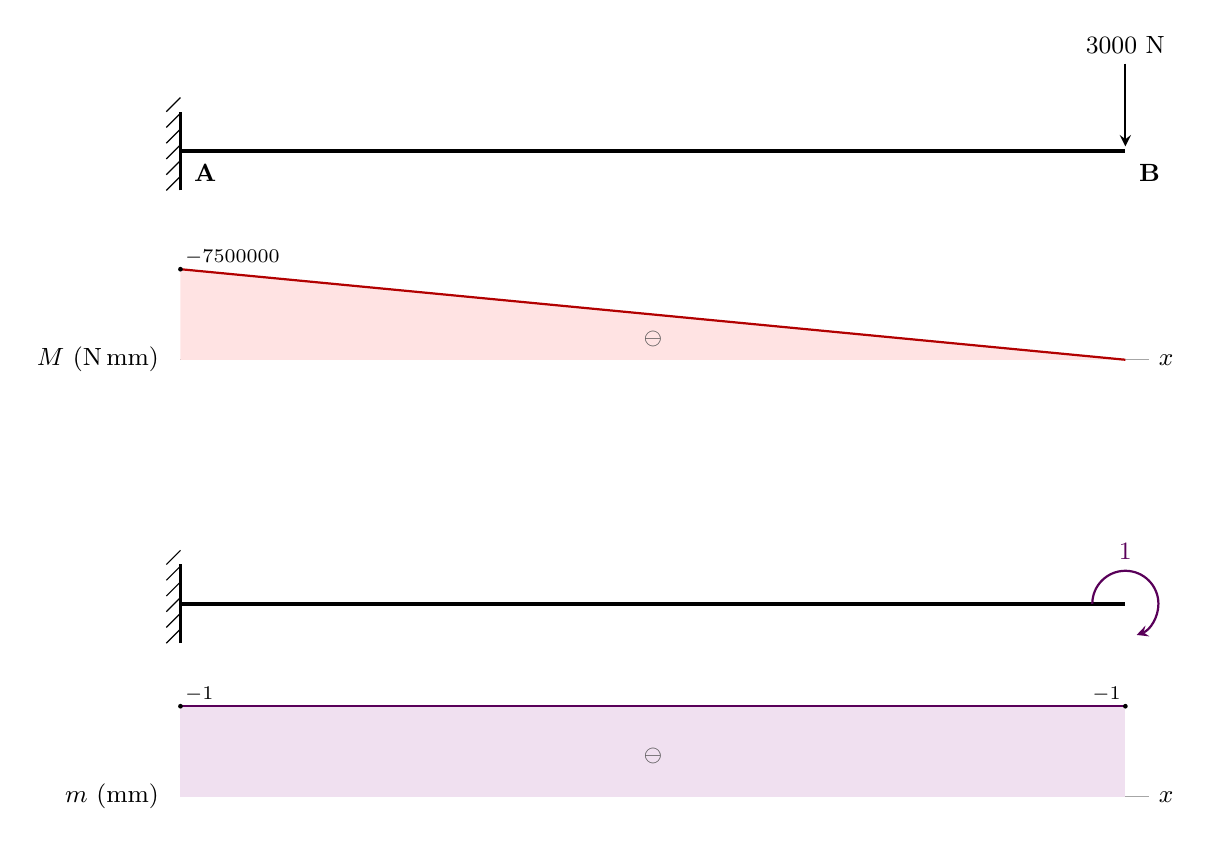
\begin{tikzpicture}
\draw[line width=1.6pt] (0,0.0000) -- (12.0000,0.0000);
% studium:at support A x=0 check=first
\draw[thick] (0.0000,-0.5000) -- (0.0000,0.5000);
\draw (0.0000,-0.3200) -- (-0.1800,-0.5000);
\draw (0.0000,-0.1200) -- (-0.1800,-0.3000);
\draw (0.0000,0.0800) -- (-0.1800,-0.1000);
\draw (0.0000,0.2800) -- (-0.1800,0.1000);
\draw (0.0000,0.4800) -- (-0.1800,0.3000);
\draw (0.0000,0.6800) -- (-0.1800,0.5000);
% studium:at force 0 x=2500 check=tip
\draw[-stealth,thick,black] (12.0000,1.1100) -- (12.0000,0.0600);
\node[font=\small,anchor=south] at (12.0000,1.1100) {$3000$~\mbox{N}};
\node[font=\small\bfseries,anchor=north west] at (0.0500,-0.0500) {A};
\node[font=\small\bfseries,anchor=north west] at (12.0500,-0.0500) {B};
\draw[gray!70] (0,-2.6500) -- (12.3000,-2.6500);
\fill[red!11] (0.0000,-2.6500) -- (0.0000,-1.5000) -- (12.0000,-2.6500) -- (12.0000,-2.6500) -- cycle;
% studium:series M sx=0.0048 sy=1.5333333333333333e-07 x0=0.0 y0=-2.65 sign=-1
\draw[thick,red!70!black] (0.0000,-1.5000) -- (12.0000,-2.6500);
% studium:end M
\node[font=\small,anchor=east] at (-0.15,-2.6500) {$M$ (N\,mm)};
\node[font=\small,anchor=west] at (12.3000,-2.6500) {$x$};
% studium:label M x=0 side=right value=-7500000
\fill (0.0000,-1.5000) circle (0.03);
\node[font=\scriptsize,anchor=south west,inner sep=1.5pt] at (0.0000,-1.5000) {$-7500000$};
\node[font=\footnotesize,gray!60!black] at (6.0000,-2.3912) {$\ominus$};
\draw[line width=1.6pt] (0,-5.7500) -- (12.0000,-5.7500);
% studium:at support A x=0 check=first
\draw[thick] (0.0000,-6.2500) -- (0.0000,-5.2500);
\draw (0.0000,-6.0700) -- (-0.1800,-6.2500);
\draw (0.0000,-5.8700) -- (-0.1800,-6.0500);
\draw (0.0000,-5.6700) -- (-0.1800,-5.8500);
\draw (0.0000,-5.4700) -- (-0.1800,-5.6500);
\draw (0.0000,-5.2700) -- (-0.1800,-5.4500);
\draw (0.0000,-5.0700) -- (-0.1800,-5.2500);
\node[font=\small,anchor=south,violet!70!black] at (12.0000,-5.3100) {$1$};
\draw[-stealth,thick,violet!70!black] (11.5800,-5.7500) arc (180:-70:0.42);
\draw[gray!70] (0,-8.2000) -- (12.3000,-8.2000);
\fill[violet!12] (0.0000,-8.2000) -- (0.0000,-7.0500) -- (12.0000,-7.0500) -- (12.0000,-8.2000) -- cycle;
% studium:series m sx=0.0048 sy=1.15 x0=0.0 y0=-8.2 sign=-1
\draw[thick,violet!70!black] (0.0000,-7.0500) -- (12.0000,-7.0500);
% studium:end m
\node[font=\small,anchor=east] at (-0.15,-8.2000) {$m$ (mm)};
\node[font=\small,anchor=west] at (12.3000,-8.2000) {$x$};
% studium:label m x=0 side=right value=-1
\fill (0.0000,-7.0500) circle (0.03);
\node[font=\scriptsize,anchor=south west,inner sep=1.5pt] at (0.0000,-7.0500) {$-1$};
% studium:label m x=2500 side=left value=-1
\fill (12.0000,-7.0500) circle (0.03);
\node[font=\scriptsize,anchor=south east,inner sep=1.5pt] at (12.0000,-7.0500) {$-1$};
\node[font=\footnotesize,gray!60!black] at (6.0000,-7.6825) {$\ominus$};
\end{tikzpicture}}%
\else
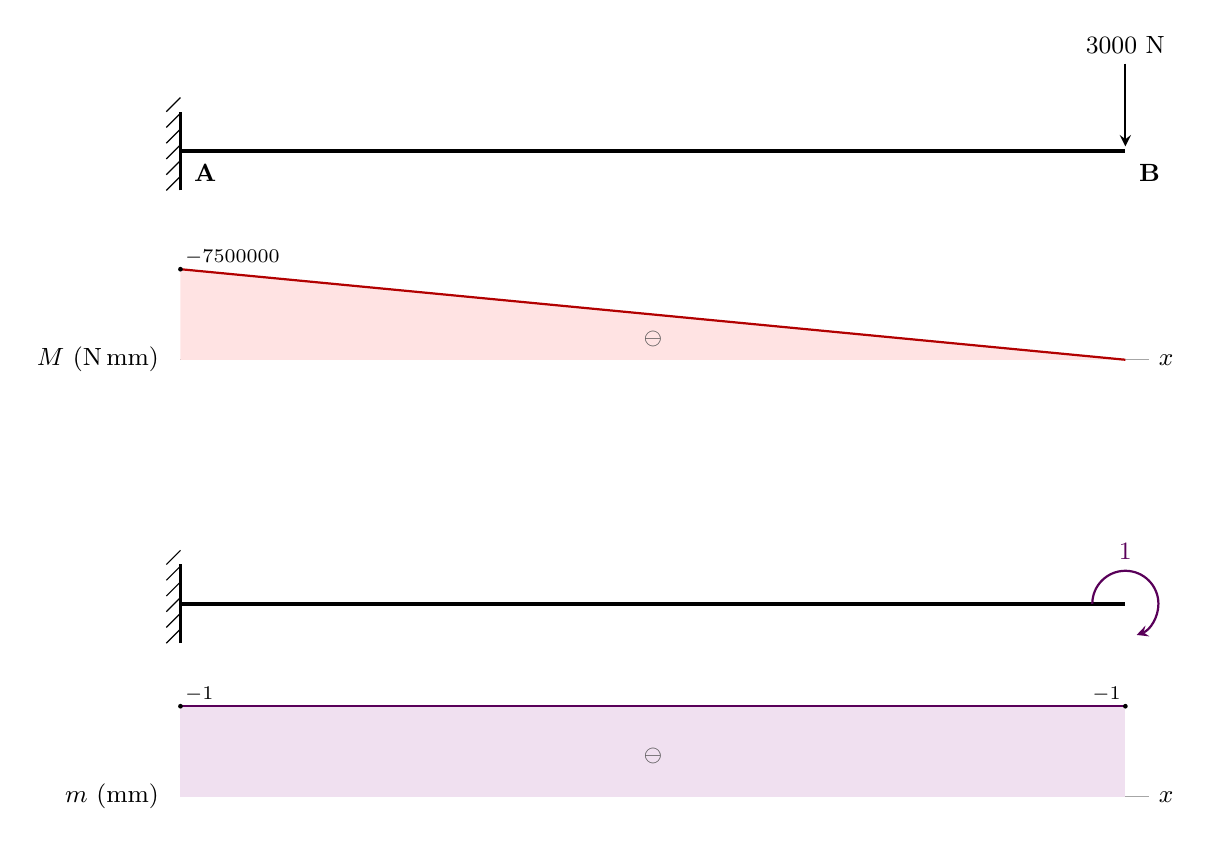
\begin{tikzpicture}
\draw[line width=1.6pt] (0,0.0000) -- (12.0000,0.0000);
% studium:at support A x=0 check=first
\draw[thick] (0.0000,-0.5000) -- (0.0000,0.5000);
\draw (0.0000,-0.3200) -- (-0.1800,-0.5000);
\draw (0.0000,-0.1200) -- (-0.1800,-0.3000);
\draw (0.0000,0.0800) -- (-0.1800,-0.1000);
\draw (0.0000,0.2800) -- (-0.1800,0.1000);
\draw (0.0000,0.4800) -- (-0.1800,0.3000);
\draw (0.0000,0.6800) -- (-0.1800,0.5000);
% studium:at force 0 x=2500 check=tip
\draw[-stealth,thick,black] (12.0000,1.1100) -- (12.0000,0.0600);
\node[font=\small,anchor=south] at (12.0000,1.1100) {$3000$~\mbox{N}};
\node[font=\small\bfseries,anchor=north west] at (0.0500,-0.0500) {A};
\node[font=\small\bfseries,anchor=north west] at (12.0500,-0.0500) {B};
\draw[gray!70] (0,-2.6500) -- (12.3000,-2.6500);
\fill[red!11] (0.0000,-2.6500) -- (0.0000,-1.5000) -- (12.0000,-2.6500) -- (12.0000,-2.6500) -- cycle;
% studium:series M sx=0.0048 sy=1.5333333333333333e-07 x0=0.0 y0=-2.65 sign=-1
\draw[thick,red!70!black] (0.0000,-1.5000) -- (12.0000,-2.6500);
% studium:end M
\node[font=\small,anchor=east] at (-0.15,-2.6500) {$M$ (N\,mm)};
\node[font=\small,anchor=west] at (12.3000,-2.6500) {$x$};
% studium:label M x=0 side=right value=-7500000
\fill (0.0000,-1.5000) circle (0.03);
\node[font=\scriptsize,anchor=south west,inner sep=1.5pt] at (0.0000,-1.5000) {$-7500000$};
\node[font=\footnotesize,gray!60!black] at (6.0000,-2.3912) {$\ominus$};
\draw[line width=1.6pt] (0,-5.7500) -- (12.0000,-5.7500);
% studium:at support A x=0 check=first
\draw[thick] (0.0000,-6.2500) -- (0.0000,-5.2500);
\draw (0.0000,-6.0700) -- (-0.1800,-6.2500);
\draw (0.0000,-5.8700) -- (-0.1800,-6.0500);
\draw (0.0000,-5.6700) -- (-0.1800,-5.8500);
\draw (0.0000,-5.4700) -- (-0.1800,-5.6500);
\draw (0.0000,-5.2700) -- (-0.1800,-5.4500);
\draw (0.0000,-5.0700) -- (-0.1800,-5.2500);
\node[font=\small,anchor=south,violet!70!black] at (12.0000,-5.3100) {$1$};
\draw[-stealth,thick,violet!70!black] (11.5800,-5.7500) arc (180:-70:0.42);
\draw[gray!70] (0,-8.2000) -- (12.3000,-8.2000);
\fill[violet!12] (0.0000,-8.2000) -- (0.0000,-7.0500) -- (12.0000,-7.0500) -- (12.0000,-8.2000) -- cycle;
% studium:series m sx=0.0048 sy=1.15 x0=0.0 y0=-8.2 sign=-1
\draw[thick,violet!70!black] (0.0000,-7.0500) -- (12.0000,-7.0500);
% studium:end m
\node[font=\small,anchor=east] at (-0.15,-8.2000) {$m$ (mm)};
\node[font=\small,anchor=west] at (12.3000,-8.2000) {$x$};
% studium:label m x=0 side=right value=-1
\fill (0.0000,-7.0500) circle (0.03);
\node[font=\scriptsize,anchor=south west,inner sep=1.5pt] at (0.0000,-7.0500) {$-1$};
% studium:label m x=2500 side=left value=-1
\fill (12.0000,-7.0500) circle (0.03);
\node[font=\scriptsize,anchor=south east,inner sep=1.5pt] at (12.0000,-7.0500) {$-1$};
\node[font=\footnotesize,gray!60!black] at (6.0000,-7.6825) {$\ominus$};
\end{tikzpicture}%
\fi
\fi
\endgroup
\par\nopagebreak
\studiumcaption{fig:e2-c07-w_giro_castigliano-trabajo-virtual}{Leyes flectoras real y virtual y carga unidad usadas en el cálculo energético.}
\end{minipage}\par\medskip

\textbf{Resultado e interpretación.}\[\fitmath{\varphi \approx 0.00261506276\,\mathrm{rad}}\]

El giro se expresa en radianes y se verifica por Castigliano con un momento auxiliar introducido antes de derivar.

\par\textbf{Comprobación.} Aplica fuerza virtual para flecha y momento virtual para giro. Mantén las cargas auxiliares hasta después de derivar y separa los tramos de distinta rigidez.

\textbf{Límites.}\begin{itemize}\item se desprecia la deformación por cortante
\item el contraste de trabajos virtuales y elástica verifica el modelo adoptado, no su idoneidad física general\end{itemize}

\textbf{Errores frecuentes.}\begin{itemize}\item emplear un único EI donde la rigidez cambia
\item confundir el momento virtual unidad (para giros) con la carga virtual unidad (para flechas)
\item olvidar un tramo al integrar las leyes flectoras\end{itemize}

\end{studiumworked}

\Needspace{.3\textheight}

\begin{studiumworked}{PRB-0239}

\section{PRB-0239 · Tensión equivalente de von mises}

\textbf{Enunciado.} Un punto de una pieza presenta $\sigma_x$ = 90 MPa, $\sigma_y$ = 110 MPa, $\sigma_z$ = 100 MPa, $\tau_{xy}$ = 15 MPa y $\tau_{xz}$ = $\tau_{yz}$ = 0. Calcule el promedio hidrostático, las tensiones principales, la tensión de von Mises y el índice de Tresca. Compare con un límite elástico de 170 MPa y explique por qué una componente hidrostática elevada no induce fluencia dúctil por sí misma.

\par\medskip\noindent\begin{tabular}{@{}p{.18\linewidth}p{.26\linewidth}p{.48\linewidth}@{}}
\toprule Símbolo & Valor y unidad & Significado\\\midrule
$\sigma_{x}$ & $90\,\mathrm{MPa}$ & tensión normal x\\
$\sigma_{y}$ & $110\,\mathrm{MPa}$ & tensión normal y\\
$\tau_{xy}$ & $15\,\mathrm{MPa}$ & cortante xy\\
$\sigma_{z}$ & $100\,\mathrm{MPa}$ & tensión normal z\\
$\sigma_{y\,fluencia}$ & $170\,\mathrm{MPa}$ & límite elástico uniaxial\\
\bottomrule\end{tabular}\par\medskip

\textbf{Hipótesis.}\begin{itemize}\item Equilibrio cuasiestático y tensor de tensiones simétrico.
\item Las tensiones sigma xz y sigma yz son nulas; sigma z es principal fuera del plano.
\item Tracción positiva y convención de signos de la Universidad de León.\end{itemize}

\textbf{Modelo y desarrollo.}

Círculo de Mohr y tensiones equivalentes.\[\fitmath{R=\sqrt{\left(\frac{\sigma_x-\sigma_y}{2}\right)^2+\tau_{xy}^{2}},\quad\sigma_{1,2}=\frac{\sigma_x+\sigma_y}{2}\pm R}\]

\textbf{Procedimiento.}\begin{itemize}\item Formar la matriz del tensor de Cauchy y obtener las tensiones principales en el plano xy.
\item Añadir la tensión normal sigma z, ordenar los tres autovalores y calcular la máxima cortadura absoluta.
\item Obtener la tensión equivalente de von Mises y la magnitud equivalente de Tresca.
\item Contrastar los resultados con los invariantes del tensor.
\item Si se proporciona el límite elástico, comparar ambos criterios de fluencia.\end{itemize}

\textbf{Cálculo de los pasos.}\begin{enumerate}

\item Centro del círculo en el plano xy.

\[\fitmath{\frac{90 + 110}{2}\approx 100\,\mathrm{MPa}}\]

\item Radio del círculo de Mohr.

\[\fitmath{\sqrt{\left(\frac{90 - 110}{2}\right)^{2} + 15^{2}}\approx 18.0277564\,\mathrm{MPa}}\]

\item Tensión principal mayor en el plano.

\[\fitmath{\sqrt{\left(\frac{90 - 110}{2}\right)^{2} + 15^{2}} + \frac{90 + 110}{2}\approx 118.027756\,\mathrm{MPa}}\]

\item Tensión principal menor en el plano.

\[\fitmath{- \sqrt{\left(\frac{90 - 110}{2}\right)^{2} + 15^{2}} + \frac{90 + 110}{2}\approx 81.9722436\,\mathrm{MPa}}\]

\item Von Mises a partir de las componentes.

\[\fitmath{\frac{\sqrt{\left(110 - 100\right)^{2} + \left(100 - 90\right)^{2} + \left(90 - 110\right)^{2} + 6 \cdot 15^{2}}}{\sqrt{2}}\approx 31.22499\,\mathrm{MPa}}\]

\item Índice tensional de Tresca.

\[\fitmath{2 \cdot 5 \sqrt{13}\approx 36.0555128\,\mathrm{MPa}}\]

\item Coeficiente de seguridad de von Mises.

\[\fitmath{\frac{170}{5 \sqrt{39}}\approx 5.44435723}\]

\item Coeficiente de seguridad de Tresca.

\[\fitmath{\frac{170}{10 \sqrt{13}}\approx 4.71495167}\]

\item Tensión media hidrostática.

\[\fitmath{\frac{90 + 100 + 110}{3}\approx 100\,\mathrm{MPa}}\]

\item Respuesta principal: comprobación final.

\[\fitmath{\frac{\sqrt{\left(110 - 100\right)^{2} + \left(100 - 90\right)^{2} + \left(90 - 110\right)^{2} + 6 \cdot 15^{2}}}{\sqrt{2}}\approx 31.22499\,\mathrm{MPa}}\]

\end{enumerate}

\textbf{Resultado e interpretación.}\[\fitmath{\begin{aligned}\sigma_{1,\mathrm{plano}} &\approx 118\,\mathrm{MPa},\quad \sigma_{2,\mathrm{plano}} \approx 81{,}97\,\mathrm{MPa}\\\sigma_{VM} &\approx 31{,}22\,\mathrm{MPa},\quad \sigma_{Tresca} \approx 36{,}06\,\mathrm{MPa}\\\sigma_{m} \approx 100\,\mathrm{MPa}\end{aligned}}\]

La parte esférica del tensor cambia las tensiones normales por igual pero no los esfuerzos equivalentes de distorsión.

\par\textbf{Comprobación.} Incluye la tercera tensión principal al evaluar Tresca y von Mises. Comprueba los invariantes antes y después de girar los ejes.

\textbf{Límites.}\begin{itemize}\item El motor solo admite cortante xy y la tensión normal z; no modela cortantes xz e yz distintos de cero.
\item El criterio de plastificación es aplicable a materiales metálicos dúctiles e isótropos.
\item Las comprobaciones reproducen el modelo indicado, no su validez constitutiva fuera del régimen elástico.\end{itemize}

\textbf{Errores frecuentes.}\begin{itemize}\item Confundir la máxima cortadura del plano xy con la máxima cortadura absoluta del tensor tridimensional.
\item Olvidar el signo de tau xy al transformar las componentes a otro plano.
\item Aplicar Tresca sin incluir la tercera tensión principal.\end{itemize}

\end{studiumworked}

\chapter{Soluciones del simulacro 3}

\objetivos{Contrasta primero el modelo y después las cifras; aplica la rúbrica del enunciado.}

\Needspace{.3\textheight}

\begin{studiumworked}{PRB-0150}

\section{PRB-0150 · Masa del tirante}

\textbf{Enunciado.} Una aleación de titanio ($E = 112{,}5$ GPa, $\rho = 4500$ kg/m$^3$) se usa para un tirante de longitud 1 m con rigidez axial $k = 2\times 10^{7}$ N/m. Calcule su masa.

\par\medskip\noindent\begin{tabular}{@{}p{.18\linewidth}p{.26\linewidth}p{.48\linewidth}@{}}
\toprule Símbolo & Valor y unidad & Significado\\\midrule
$k$ & $20\,\mathrm{kN/mm}$ & rigidez axial\\
$L$ & $1.0\,\mathrm{m}$ & longitud\\
$E$ & $112.5\,\mathrm{GPa}$ & módulo del titanio\\
$\rho$ & $4500\,\mathrm{kg/m^3}$ & densidad\\
\bottomrule\end{tabular}\par\medskip

\textbf{Hipótesis.}\begin{itemize}\item barra prismática homogénea
\item diseño gobernado por la rigidez\end{itemize}

\textbf{Modelo y desarrollo.}

Masa de un tirante de rigidez dada.\[\fitmath{m = \frac{\rho\,k\,L^{2}}{E}}\]

\textbf{Procedimiento.}\begin{itemize}\item La masa es $m = \rho k L^2/E$.\end{itemize}

\textbf{Cálculo de los pasos.}\begin{enumerate}

\item Masa del tirante.

\[\fitmath{4500 \cdot 20000000.0 {1.0}^{2} \frac{1}{112500000000.0}\approx 0.8\,\mathrm{kg}}\]

\end{enumerate}

\textbf{Resultado e interpretación.}\[\fitmath{m = 0{,}800\ \mathrm{kg}}\]

Con $\rho/E$ del orden de $4\times 10^{-8}$ s$^2$/m$^2$ la masa sale cercana a la del aluminio y la del acero.

\par\textbf{Comprobación.} Reconstruye el área desde la rigidez axial y comprueba la masa con la densidad; compara a igual rigidez y longitud.

\textbf{Límites.}\begin{itemize}\item no incluye uniones\end{itemize}

\textbf{Errores frecuentes.}\begin{itemize}\item olvidar elevar la longitud al cuadrado\end{itemize}

\end{studiumworked}

\Needspace{.3\textheight}

\begin{studiumworked}{PRB-0192}

\section{PRB-0192 · Flector máximo}

\textbf{Enunciado.} Una viga biapoyada de 5 m soporta dos cargas puntuales hacia abajo: 10 kN a 1 m del apoyo izquierdo $A$ y 20 kN a 3 m. Dibuje los diagramas de cortantes y flectores y calcule el flector máximo.

\par\medskip\noindent\begin{tabular}{@{}p{.18\linewidth}p{.26\linewidth}p{.48\linewidth}@{}}
\toprule Símbolo & Valor y unidad & Significado\\\midrule
$L$ & $5\,\mathrm{m}$ & luz\\
\bottomrule\end{tabular}\par\medskip

\textbf{Hipótesis.}\begin{itemize}\item criterio de signos del curso\end{itemize}

\textbf{Modelo y desarrollo.}

Equilibrio de la viga.\[\fitmath{\sum F_y = 0,\qquad \sum M = 0}\]

\textbf{Cálculo de los pasos.}\begin{enumerate}

\item Reacción en B.

\[\fitmath{\frac{10 \cdot 1 + 20 \cdot 3}{5}\approx 14\,\mathrm{kN}}\]

\item Reacción en A.

\[\fitmath{30 - 14\approx 16\,\mathrm{kN}}\]

\item Flector máximo, bajo la carga de 20 kN.

\[\fitmath{14 \cdot 2\approx 28\,\mathrm{kN\,m}}\]

\end{enumerate}

\textbf{Resultado e interpretación.}\[\fitmath{M_{z,\max} = 28\ \mathrm{kN\,m}\ (x = 3\ \mathrm{m})}\]

Sin cargas repartidas el cortante es constante entre cargas y el flector es lineal; el máximo está bajo la carga en la que el cortante pasa de positivo a negativo.

\par\textbf{Comprobación.} Verifica las tres ecuaciones de equilibrio, los saltos de cortante y momento y las condiciones de cada apoyo o rótula.

\textbf{Límites.}\begin{itemize}\item no se incluye el peso propio\end{itemize}

\textbf{Errores frecuentes.}\begin{itemize}\item buscar el máximo en el centro de la luz\end{itemize}

\end{studiumworked}

\Needspace{.3\textheight}

\begin{studiumworked}{PRB-0165}

\section{PRB-0165 · Giro entre extremos}

\textbf{Enunciado.} Un árbol tubular de aleación 7075 ($G = 26{,}95$ GPa) tiene un radio exterior de 25 mm, un radio interior de 20 mm y una longitud de 1 m. Transmite un torsor constante de 1 kN$\cdot$m. Calcule la constante de torsión, la tensión tangencial máxima y el giro entre los extremos.

\par\medskip\noindent\begin{tabular}{@{}p{.18\linewidth}p{.26\linewidth}p{.48\linewidth}@{}}
\toprule Símbolo & Valor y unidad & Significado\\\midrule
$R_{e}$ & $25\,\mathrm{mm}$ & radio exterior\\
$R_{i}$ & $20\,\mathrm{mm}$ & radio interior\\
$L$ & $1000\,\mathrm{mm}$ & longitud\\
$M_{x}$ & $1000\,\mathrm{N\,m}$ & torsor\\
$G$ & $26950\,\mathrm{MPa}$ & módulo transversal del 7075\\
\bottomrule\end{tabular}\par\medskip

\textbf{Hipótesis.}\begin{itemize}\item tubo circular de sección constante
\item torsor constante
\item material elástico lineal\end{itemize}

\textbf{Modelo y desarrollo.}

Giro de un tubo circular.\[\fitmath{\theta_x = \frac{M_x\,L}{G\,J},\quad J = \frac{\pi}{2}\left(R_e^{4} - R_i^{4}\right)}\]

\textbf{Procedimiento.}\begin{itemize}\item La constante de torsión es el momento de inercia polar de la corona.
\item La tensión máxima está en el radio exterior.
\item El giro total es el giro unitario por la longitud.\end{itemize}

\textbf{Cálculo de los pasos.}\begin{enumerate}

\item Constante de torsión.

\[\fitmath{\frac{\pi \left(- 20^{4} + 25^{4}\right)}{2}\approx 3.6226\times10^{5}\,\mathrm{mm^4}}\]

\item Tensión tangencial máxima.

\[\fitmath{1000000.0 \cdot 25 \frac{1}{\frac{1}{2} \pi \left(- 20^{4} + 25^{4}\right)}\approx 69.01\,\mathrm{MPa}}\]

\item Giro entre extremos.

\[\fitmath{1000000.0 \cdot 1000 \frac{1}{26950 \cdot \frac{1}{2} \pi \left(- 20^{4} + 25^{4}\right)}\approx 0.1024\,\mathrm{rad}}\]

\end{enumerate}

\textbf{Resultado e interpretación.}\[\fitmath{J \approx 3{,}62\times 10^{5}\ \mathrm{mm}^{4},\quad \tau_{max} \approx 69{,}0\ \mathrm{MPa},\quad \theta_x \approx 0{,}102\ \mathrm{rad}}\]

El giro de $0{,}102$ rad equivale a $5{,}9$ grados en un metro de árbol. El cálculo supone comportamiento elástico lineal. No se verifica el límite elástico de la aleación, porque no se especifica su estado de tratamiento ni se aporta una tensión admisible a cortadura.

\par\textbf{Comprobación.} Distingue secciones abiertas y cerradas: la constante torsional de tiras abiertas no es el momento polar. En multiceldas, exige equilibrio y giro compatible.

\textbf{Límites.}\begin{itemize}\item no incluye la flexión ni los extremos de la barra\end{itemize}

\textbf{Errores frecuentes.}\begin{itemize}\item usar el diámetro en lugar del radio
\item usar el módulo de Young en lugar del módulo transversal\end{itemize}

\end{studiumworked}

\Needspace{.3\textheight}

\begin{studiumworked}{PRB-0224}

\section{PRB-0224 · Flecha en la sección indicada}

\textbf{Enunciado.} Una viga biapoyada de 5 m tiene una carga vertical de 6 kN aplicada a 2 m del apoyo izquierdo. Con E = 71,7 GPa e I = 5,0·10\textsuperscript{7} mm$^4$, calcule mediante una fuerza virtual unidad la flecha en el punto de carga; represente los diagramas flectores real y virtual.

\par\medskip\noindent\begin{tabular}{@{}p{.18\linewidth}p{.26\linewidth}p{.48\linewidth}@{}}
\toprule Símbolo & Valor y unidad & Significado\\\midrule
$L$ & $5000\,\mathrm{mm}$ & longitud de la viga\\
$E$ & $71700\,\mathrm{MPa}$ & módulo de Young\\
$EI$ & $3585000000000\,\mathrm{N\,mm^2}$ & rigidez a flexión\\
\bottomrule\end{tabular}\par\medskip

\par\medskip\noindent\begin{minipage}{\linewidth}
\centering
\begingroup
\setbox0=\hbox{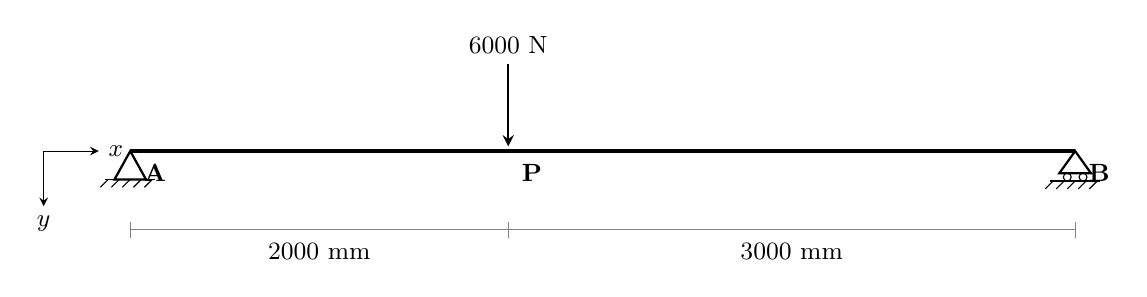
\begin{tikzpicture}
\draw[line width=1.6pt] (0,0.0000) -- (12.0000,0.0000);
% studium:at support A x=0 check=first
\draw[thick,fill=white] (0.0000,0.0000) -- (-0.2000,-0.3600) -- (0.2000,-0.3600) -- cycle;
\draw (-0.3200,-0.3600) -- (0.3200,-0.3600);
\draw (-0.2800,-0.3600) -- (-0.3800,-0.4600);
\draw (-0.1400,-0.3600) -- (-0.2400,-0.4600);
\draw (0.0000,-0.3600) -- (-0.1000,-0.4600);
\draw (0.1400,-0.3600) -- (0.0400,-0.4600);
\draw (0.2800,-0.3600) -- (0.1800,-0.4600);
% studium:at support B x=5000 check=first
\draw[thick,fill=white] (12.0000,0.0000) -- (11.8000,-0.2800) -- (12.2000,-0.2800) -- cycle;
\draw (11.9000,-0.3300) circle (0.05);
\draw (12.1000,-0.3300) circle (0.05);
\draw (11.6800,-0.3800) -- (12.3200,-0.3800);
\draw (11.7200,-0.3800) -- (11.6200,-0.4800);
\draw (11.8600,-0.3800) -- (11.7600,-0.4800);
\draw (12.0000,-0.3800) -- (11.9000,-0.4800);
\draw (12.1400,-0.3800) -- (12.0400,-0.4800);
\draw (12.2800,-0.3800) -- (12.1800,-0.4800);
% studium:at force 0 x=2000 check=tip
\draw[-stealth,thick,black] (4.8000,1.1100) -- (4.8000,0.0600);
\node[font=\small,anchor=south] at (4.8000,1.1100) {$6000$~\mbox{N}};
\node[font=\small\bfseries,anchor=north west] at (0.0500,-0.0500) {A};
\node[font=\small\bfseries,anchor=north west] at (4.8500,-0.0500) {P};
\node[font=\small\bfseries,anchor=north west] at (12.0500,-0.0500) {B};
\draw[gray] (0,-1.0000) -- (12.0000,-1.0000);
\draw[gray] (0.0000,-1.1000) -- (0.0000,-0.9000);
\draw[gray] (4.8000,-1.1000) -- (4.8000,-0.9000);
\draw[gray] (12.0000,-1.1000) -- (12.0000,-0.9000);
\node[font=\small,anchor=north] at (2.4000,-1.0500) {$2000$~\mbox{mm}};
\node[font=\small,anchor=north] at (8.4000,-1.0500) {$3000$~\mbox{mm}};
\draw[-stealth] (-1.1,0.0000) -- (-0.4,0.0000) node[right,font=\small] {$x$};
\draw[-stealth] (-1.1,0.0000) -- (-1.1,-0.7000) node[below,font=\small] {$y$};
\end{tikzpicture}}%
\count0=\ht0
\advance\count0 by \dp0
\count2=\wd0
\count4=\dimexpr\textheight/100*38\relax
\count6=\linewidth
\ifnum\count0<1
\count0=1
\fi
\ifnum\count2<1
\count2=1
\fi
\divide\count0 by 4096
\divide\count2 by 4096
\divide\count4 by 4096
\divide\count6 by 4096
\ifnum\count0<1
\count0=1
\fi
\ifnum\count2<1
\count2=1
\fi
\ifnum\count4<1
\count4=1
\fi
\ifnum\count6<1
\count6=1
\fi
\count8=\count2
\ifnum\count0>\count4
\count8=\numexpr\count2*\count4/\count0\relax
\fi
\ifnum\count8>\count6
\resizebox{\linewidth}{!}{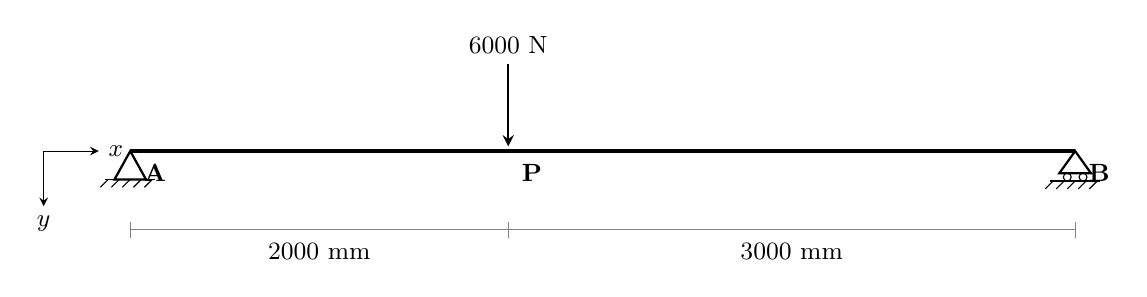
\begin{tikzpicture}
\draw[line width=1.6pt] (0,0.0000) -- (12.0000,0.0000);
% studium:at support A x=0 check=first
\draw[thick,fill=white] (0.0000,0.0000) -- (-0.2000,-0.3600) -- (0.2000,-0.3600) -- cycle;
\draw (-0.3200,-0.3600) -- (0.3200,-0.3600);
\draw (-0.2800,-0.3600) -- (-0.3800,-0.4600);
\draw (-0.1400,-0.3600) -- (-0.2400,-0.4600);
\draw (0.0000,-0.3600) -- (-0.1000,-0.4600);
\draw (0.1400,-0.3600) -- (0.0400,-0.4600);
\draw (0.2800,-0.3600) -- (0.1800,-0.4600);
% studium:at support B x=5000 check=first
\draw[thick,fill=white] (12.0000,0.0000) -- (11.8000,-0.2800) -- (12.2000,-0.2800) -- cycle;
\draw (11.9000,-0.3300) circle (0.05);
\draw (12.1000,-0.3300) circle (0.05);
\draw (11.6800,-0.3800) -- (12.3200,-0.3800);
\draw (11.7200,-0.3800) -- (11.6200,-0.4800);
\draw (11.8600,-0.3800) -- (11.7600,-0.4800);
\draw (12.0000,-0.3800) -- (11.9000,-0.4800);
\draw (12.1400,-0.3800) -- (12.0400,-0.4800);
\draw (12.2800,-0.3800) -- (12.1800,-0.4800);
% studium:at force 0 x=2000 check=tip
\draw[-stealth,thick,black] (4.8000,1.1100) -- (4.8000,0.0600);
\node[font=\small,anchor=south] at (4.8000,1.1100) {$6000$~\mbox{N}};
\node[font=\small\bfseries,anchor=north west] at (0.0500,-0.0500) {A};
\node[font=\small\bfseries,anchor=north west] at (4.8500,-0.0500) {P};
\node[font=\small\bfseries,anchor=north west] at (12.0500,-0.0500) {B};
\draw[gray] (0,-1.0000) -- (12.0000,-1.0000);
\draw[gray] (0.0000,-1.1000) -- (0.0000,-0.9000);
\draw[gray] (4.8000,-1.1000) -- (4.8000,-0.9000);
\draw[gray] (12.0000,-1.1000) -- (12.0000,-0.9000);
\node[font=\small,anchor=north] at (2.4000,-1.0500) {$2000$~\mbox{mm}};
\node[font=\small,anchor=north] at (8.4000,-1.0500) {$3000$~\mbox{mm}};
\draw[-stealth] (-1.1,0.0000) -- (-0.4,0.0000) node[right,font=\small] {$x$};
\draw[-stealth] (-1.1,0.0000) -- (-1.1,-0.7000) node[below,font=\small] {$y$};
\end{tikzpicture}}%
\else
\ifnum\count0>\count4
\resizebox{!}{\dimexpr\textheight/100*38\relax}{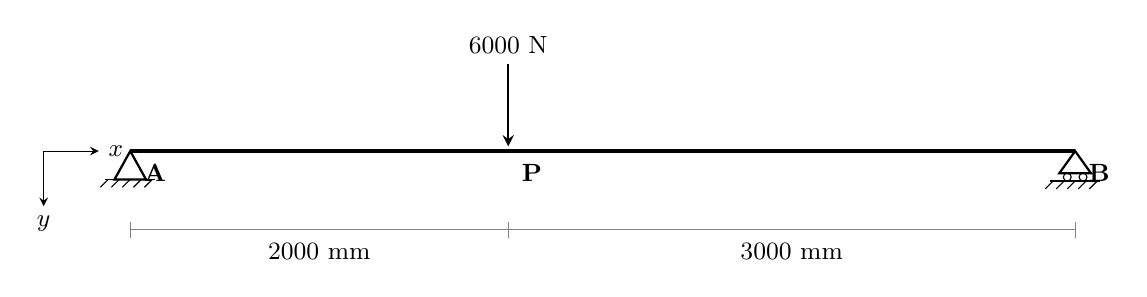
\begin{tikzpicture}
\draw[line width=1.6pt] (0,0.0000) -- (12.0000,0.0000);
% studium:at support A x=0 check=first
\draw[thick,fill=white] (0.0000,0.0000) -- (-0.2000,-0.3600) -- (0.2000,-0.3600) -- cycle;
\draw (-0.3200,-0.3600) -- (0.3200,-0.3600);
\draw (-0.2800,-0.3600) -- (-0.3800,-0.4600);
\draw (-0.1400,-0.3600) -- (-0.2400,-0.4600);
\draw (0.0000,-0.3600) -- (-0.1000,-0.4600);
\draw (0.1400,-0.3600) -- (0.0400,-0.4600);
\draw (0.2800,-0.3600) -- (0.1800,-0.4600);
% studium:at support B x=5000 check=first
\draw[thick,fill=white] (12.0000,0.0000) -- (11.8000,-0.2800) -- (12.2000,-0.2800) -- cycle;
\draw (11.9000,-0.3300) circle (0.05);
\draw (12.1000,-0.3300) circle (0.05);
\draw (11.6800,-0.3800) -- (12.3200,-0.3800);
\draw (11.7200,-0.3800) -- (11.6200,-0.4800);
\draw (11.8600,-0.3800) -- (11.7600,-0.4800);
\draw (12.0000,-0.3800) -- (11.9000,-0.4800);
\draw (12.1400,-0.3800) -- (12.0400,-0.4800);
\draw (12.2800,-0.3800) -- (12.1800,-0.4800);
% studium:at force 0 x=2000 check=tip
\draw[-stealth,thick,black] (4.8000,1.1100) -- (4.8000,0.0600);
\node[font=\small,anchor=south] at (4.8000,1.1100) {$6000$~\mbox{N}};
\node[font=\small\bfseries,anchor=north west] at (0.0500,-0.0500) {A};
\node[font=\small\bfseries,anchor=north west] at (4.8500,-0.0500) {P};
\node[font=\small\bfseries,anchor=north west] at (12.0500,-0.0500) {B};
\draw[gray] (0,-1.0000) -- (12.0000,-1.0000);
\draw[gray] (0.0000,-1.1000) -- (0.0000,-0.9000);
\draw[gray] (4.8000,-1.1000) -- (4.8000,-0.9000);
\draw[gray] (12.0000,-1.1000) -- (12.0000,-0.9000);
\node[font=\small,anchor=north] at (2.4000,-1.0500) {$2000$~\mbox{mm}};
\node[font=\small,anchor=north] at (8.4000,-1.0500) {$3000$~\mbox{mm}};
\draw[-stealth] (-1.1,0.0000) -- (-0.4,0.0000) node[right,font=\small] {$x$};
\draw[-stealth] (-1.1,0.0000) -- (-1.1,-0.7000) node[below,font=\small] {$y$};
\end{tikzpicture}}%
\else
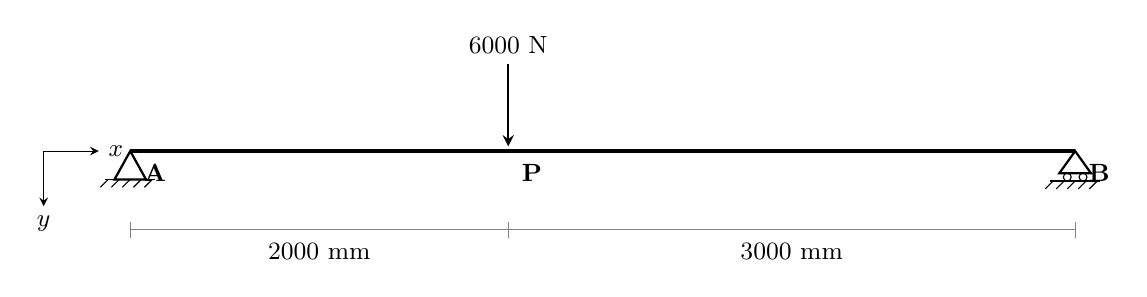
\begin{tikzpicture}
\draw[line width=1.6pt] (0,0.0000) -- (12.0000,0.0000);
% studium:at support A x=0 check=first
\draw[thick,fill=white] (0.0000,0.0000) -- (-0.2000,-0.3600) -- (0.2000,-0.3600) -- cycle;
\draw (-0.3200,-0.3600) -- (0.3200,-0.3600);
\draw (-0.2800,-0.3600) -- (-0.3800,-0.4600);
\draw (-0.1400,-0.3600) -- (-0.2400,-0.4600);
\draw (0.0000,-0.3600) -- (-0.1000,-0.4600);
\draw (0.1400,-0.3600) -- (0.0400,-0.4600);
\draw (0.2800,-0.3600) -- (0.1800,-0.4600);
% studium:at support B x=5000 check=first
\draw[thick,fill=white] (12.0000,0.0000) -- (11.8000,-0.2800) -- (12.2000,-0.2800) -- cycle;
\draw (11.9000,-0.3300) circle (0.05);
\draw (12.1000,-0.3300) circle (0.05);
\draw (11.6800,-0.3800) -- (12.3200,-0.3800);
\draw (11.7200,-0.3800) -- (11.6200,-0.4800);
\draw (11.8600,-0.3800) -- (11.7600,-0.4800);
\draw (12.0000,-0.3800) -- (11.9000,-0.4800);
\draw (12.1400,-0.3800) -- (12.0400,-0.4800);
\draw (12.2800,-0.3800) -- (12.1800,-0.4800);
% studium:at force 0 x=2000 check=tip
\draw[-stealth,thick,black] (4.8000,1.1100) -- (4.8000,0.0600);
\node[font=\small,anchor=south] at (4.8000,1.1100) {$6000$~\mbox{N}};
\node[font=\small\bfseries,anchor=north west] at (0.0500,-0.0500) {A};
\node[font=\small\bfseries,anchor=north west] at (4.8500,-0.0500) {P};
\node[font=\small\bfseries,anchor=north west] at (12.0500,-0.0500) {B};
\draw[gray] (0,-1.0000) -- (12.0000,-1.0000);
\draw[gray] (0.0000,-1.1000) -- (0.0000,-0.9000);
\draw[gray] (4.8000,-1.1000) -- (4.8000,-0.9000);
\draw[gray] (12.0000,-1.1000) -- (12.0000,-0.9000);
\node[font=\small,anchor=north] at (2.4000,-1.0500) {$2000$~\mbox{mm}};
\node[font=\small,anchor=north] at (8.4000,-1.0500) {$3000$~\mbox{mm}};
\draw[-stealth] (-1.1,0.0000) -- (-0.4,0.0000) node[right,font=\small] {$x$};
\draw[-stealth] (-1.1,0.0000) -- (-1.1,-0.7000) node[below,font=\small] {$y$};
\end{tikzpicture}%
\fi
\fi
\endgroup
\par\nopagebreak
\studiumcaption{fig:e2-c07-w_carga_descentrada-enunciado}{Viga real: apoyos, cargas y distancias conocidas, sin reacciones calculadas.}
\end{minipage}\par\medskip

\textbf{Hipótesis.}\begin{itemize}\item respuesta elástica lineal y pequeños desplazamientos
\item teoría de Euler-Bernoulli, sin contribución de energía por cortante
\item módulo E y rigideces EI según enunciado
\item convenio de signos de la ULE\end{itemize}

\textbf{Modelo y desarrollo.}

Trabajo virtual de flexión.\[\fitmath{\delta = \int_{0}^{L}\frac{M(x)\,\overline{M}(x)}{E I(x)}\,\mathrm{d}x}\]

\textbf{Procedimiento.}\begin{itemize}\item Calcular las reacciones del caso real mediante equilibrio y, en su caso, compatibilidad de flechas.
\item Escribir la ley flectora real M(x) en cada intervalo.
\item Introducir una fuerza virtual unidad en el punto y sentido del desplazamiento buscado.
\item Calcular la ley flectora virtual y sumar las integrales de M por M virtual dividido entre EI para todos los tramos.
\item Verificar el resultado mediante la elástica calculada con constantes de integración y condiciones de apoyo.
\item La posición de la carga no está en el centro: dividir las integrales en los dos tramos; contrastar con el resultado de Castigliano P a\textsuperscript{2} b\textsuperscript{2}/(3 L E I).\end{itemize}

\textbf{Cálculo de los pasos.}\begin{enumerate}

\item Integral M por M virtual dividida por EI, tramo 1: 0 a 2000 mm.

\[\fitmath{\frac{5760000000000}{3585000000000}\approx 1.60669456\,\mathrm{mm}}\]

\item Integral M por M virtual dividida por EI, tramo 2: 2000 a 5000 mm.

\[\fitmath{\frac{8640000000000}{3585000000000}\approx 2.41004184\,\mathrm{mm}}\]

\item Desplazamiento total por suma de tramos.

\[\fitmath{\frac{5760000000000}{3585000000000} + \frac{8640000000000}{3585000000000}\approx 4.0167364\,\mathrm{mm}}\]

\end{enumerate}

\par\medskip\noindent\begin{minipage}{\linewidth}
\centering
\begingroup
\setbox0=\hbox{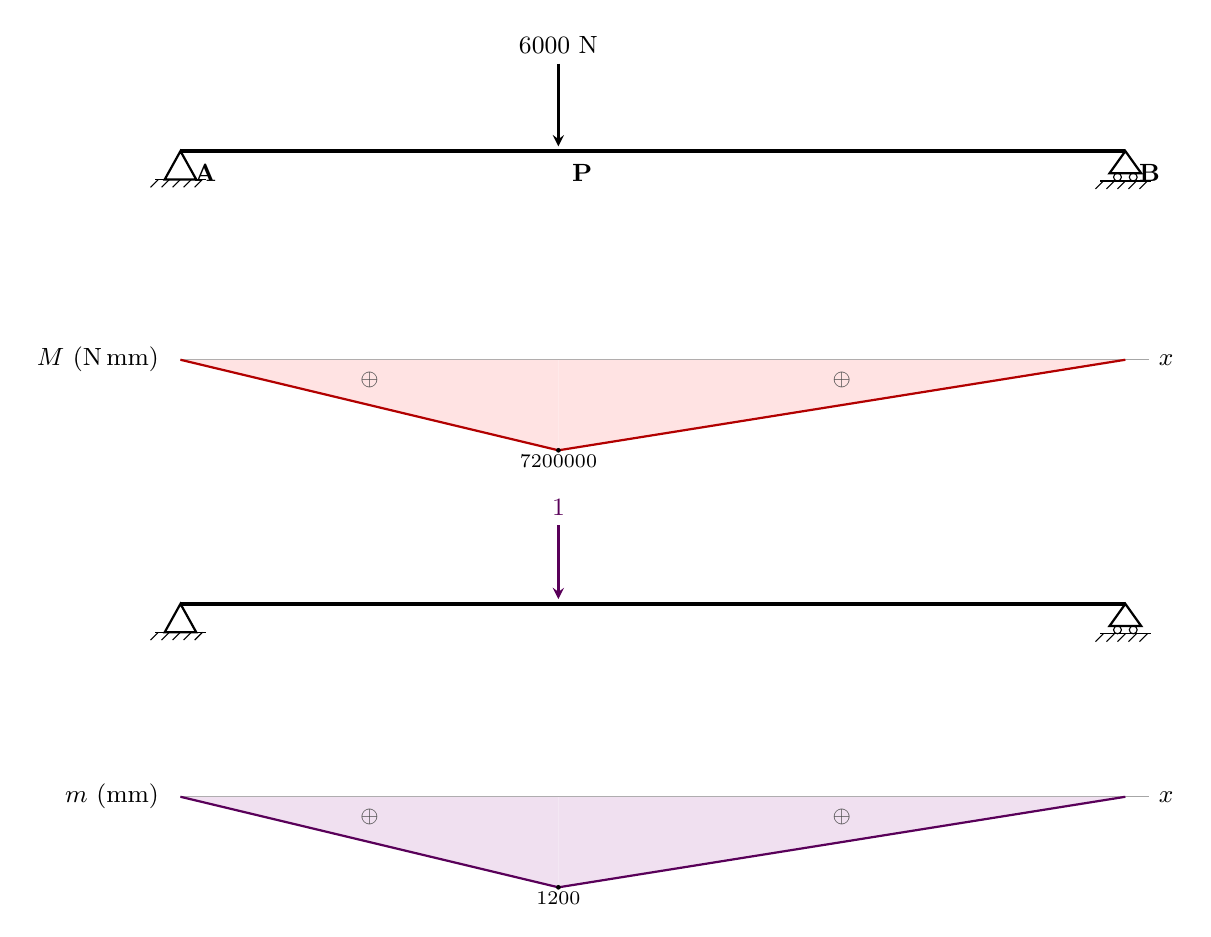
\begin{tikzpicture}
\draw[line width=1.6pt] (0,0.0000) -- (12.0000,0.0000);
% studium:at support A x=0 check=first
\draw[thick,fill=white] (0.0000,0.0000) -- (-0.2000,-0.3600) -- (0.2000,-0.3600) -- cycle;
\draw (-0.3200,-0.3600) -- (0.3200,-0.3600);
\draw (-0.2800,-0.3600) -- (-0.3800,-0.4600);
\draw (-0.1400,-0.3600) -- (-0.2400,-0.4600);
\draw (0.0000,-0.3600) -- (-0.1000,-0.4600);
\draw (0.1400,-0.3600) -- (0.0400,-0.4600);
\draw (0.2800,-0.3600) -- (0.1800,-0.4600);
% studium:at support B x=5000 check=first
\draw[thick,fill=white] (12.0000,0.0000) -- (11.8000,-0.2800) -- (12.2000,-0.2800) -- cycle;
\draw (11.9000,-0.3300) circle (0.05);
\draw (12.1000,-0.3300) circle (0.05);
\draw (11.6800,-0.3800) -- (12.3200,-0.3800);
\draw (11.7200,-0.3800) -- (11.6200,-0.4800);
\draw (11.8600,-0.3800) -- (11.7600,-0.4800);
\draw (12.0000,-0.3800) -- (11.9000,-0.4800);
\draw (12.1400,-0.3800) -- (12.0400,-0.4800);
\draw (12.2800,-0.3800) -- (12.1800,-0.4800);
% studium:at force 0 x=2000 check=tip
\draw[-stealth,thick,black] (4.8000,1.1100) -- (4.8000,0.0600);
\node[font=\small,anchor=south] at (4.8000,1.1100) {$6000$~\mbox{N}};
\node[font=\small\bfseries,anchor=north west] at (0.0500,-0.0500) {A};
\node[font=\small\bfseries,anchor=north west] at (4.8500,-0.0500) {P};
\node[font=\small\bfseries,anchor=north west] at (12.0500,-0.0500) {B};
\draw[gray!70] (0,-2.6500) -- (12.3000,-2.6500);
\fill[red!11] (0.0000,-2.6500) -- (0.0000,-2.6500) -- (4.8000,-3.8000) -- (4.8000,-2.6500) -- cycle;
\fill[red!11] (4.8000,-2.6500) -- (4.8000,-3.8000) -- (12.0000,-2.6500) -- (12.0000,-2.6500) -- cycle;
% studium:series M sx=0.0024 sy=1.597222222222222e-07 x0=0.0 y0=-2.65 sign=-1
\draw[thick,red!70!black] (0.0000,-2.6500) -- (4.8000,-3.8000);
\draw[thick,red!70!black] (4.8000,-3.8000) -- (12.0000,-2.6500);
% studium:end M
\node[font=\small,anchor=east] at (-0.15,-2.6500) {$M$ (N\,mm)};
\node[font=\small,anchor=west] at (12.3000,-2.6500) {$x$};
% studium:label M x=2000 side=both value=7200000
\fill (4.8000,-3.8000) circle (0.03);
\node[font=\scriptsize,anchor=north,inner sep=1.5pt] at (4.8000,-3.8000) {$7200000$};
\node[font=\footnotesize,gray!60!black] at (2.4000,-2.9087) {$\oplus$};
\node[font=\footnotesize,gray!60!black] at (8.4000,-2.9087) {$\oplus$};
\draw[line width=1.6pt] (0,-5.7500) -- (12.0000,-5.7500);
% studium:at support A x=0 check=first
\draw[thick,fill=white] (0.0000,-5.7500) -- (-0.2000,-6.1100) -- (0.2000,-6.1100) -- cycle;
\draw (-0.3200,-6.1100) -- (0.3200,-6.1100);
\draw (-0.2800,-6.1100) -- (-0.3800,-6.2100);
\draw (-0.1400,-6.1100) -- (-0.2400,-6.2100);
\draw (0.0000,-6.1100) -- (-0.1000,-6.2100);
\draw (0.1400,-6.1100) -- (0.0400,-6.2100);
\draw (0.2800,-6.1100) -- (0.1800,-6.2100);
% studium:at support B x=5000 check=first
\draw[thick,fill=white] (12.0000,-5.7500) -- (11.8000,-6.0300) -- (12.2000,-6.0300) -- cycle;
\draw (11.9000,-6.0800) circle (0.05);
\draw (12.1000,-6.0800) circle (0.05);
\draw (11.6800,-6.1300) -- (12.3200,-6.1300);
\draw (11.7200,-6.1300) -- (11.6200,-6.2300);
\draw (11.8600,-6.1300) -- (11.7600,-6.2300);
\draw (12.0000,-6.1300) -- (11.9000,-6.2300);
\draw (12.1400,-6.1300) -- (12.0400,-6.2300);
\draw (12.2800,-6.1300) -- (12.1800,-6.2300);
\draw[-stealth,thick,violet!70!black] (4.8000,-4.7500) -- (4.8000,-5.6900);
\node[font=\small,violet!70!black,anchor=south] at (4.8000,-4.7500) {$1$};
\draw[gray!70] (0,-8.2000) -- (12.3000,-8.2000);
\fill[violet!12] (0.0000,-8.2000) -- (0.0000,-8.2000) -- (4.8000,-9.3500) -- (4.8000,-8.2000) -- cycle;
\fill[violet!12] (4.8000,-8.2000) -- (4.8000,-9.3500) -- (12.0000,-8.2000) -- (12.0000,-8.2000) -- cycle;
% studium:series m sx=0.0024 sy=0.0009583333333333333 x0=0.0 y0=-8.2 sign=-1
\draw[thick,violet!70!black] (0.0000,-8.2000) -- (4.8000,-9.3500);
\draw[thick,violet!70!black] (4.8000,-9.3500) -- (12.0000,-8.2000);
% studium:end m
\node[font=\small,anchor=east] at (-0.15,-8.2000) {$m$ (mm)};
\node[font=\small,anchor=west] at (12.3000,-8.2000) {$x$};
% studium:label m x=2000 side=both value=1200
\fill (4.8000,-9.3500) circle (0.03);
\node[font=\scriptsize,anchor=north,inner sep=1.5pt] at (4.8000,-9.3500) {$1200$};
\node[font=\footnotesize,gray!60!black] at (2.4000,-8.4587) {$\oplus$};
\node[font=\footnotesize,gray!60!black] at (8.4000,-8.4587) {$\oplus$};
\end{tikzpicture}}%
\count0=\ht0
\advance\count0 by \dp0
\count2=\wd0
\count4=\dimexpr\textheight/100*38\relax
\count6=\linewidth
\ifnum\count0<1
\count0=1
\fi
\ifnum\count2<1
\count2=1
\fi
\divide\count0 by 4096
\divide\count2 by 4096
\divide\count4 by 4096
\divide\count6 by 4096
\ifnum\count0<1
\count0=1
\fi
\ifnum\count2<1
\count2=1
\fi
\ifnum\count4<1
\count4=1
\fi
\ifnum\count6<1
\count6=1
\fi
\count8=\count2
\ifnum\count0>\count4
\count8=\numexpr\count2*\count4/\count0\relax
\fi
\ifnum\count8>\count6
\resizebox{\linewidth}{!}{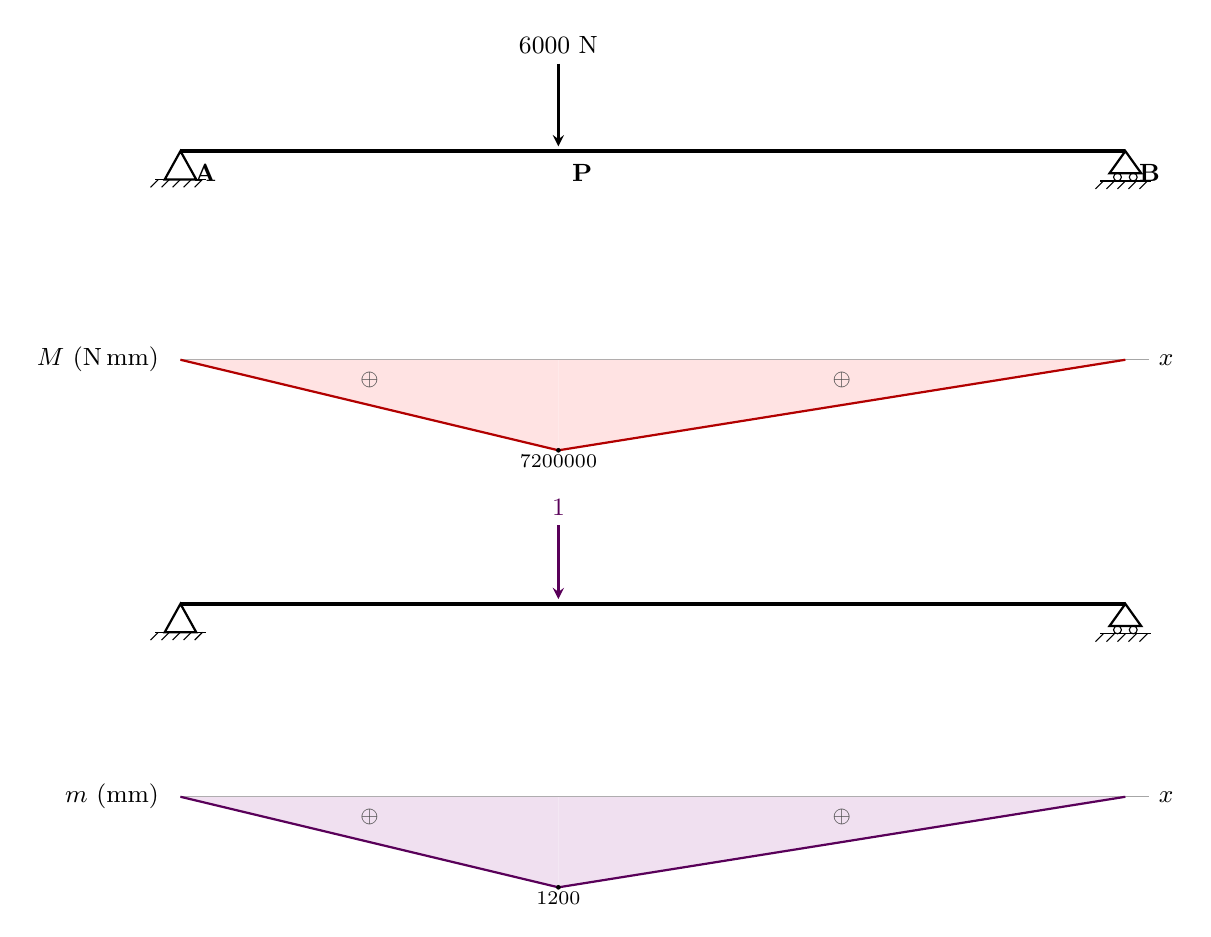
\begin{tikzpicture}
\draw[line width=1.6pt] (0,0.0000) -- (12.0000,0.0000);
% studium:at support A x=0 check=first
\draw[thick,fill=white] (0.0000,0.0000) -- (-0.2000,-0.3600) -- (0.2000,-0.3600) -- cycle;
\draw (-0.3200,-0.3600) -- (0.3200,-0.3600);
\draw (-0.2800,-0.3600) -- (-0.3800,-0.4600);
\draw (-0.1400,-0.3600) -- (-0.2400,-0.4600);
\draw (0.0000,-0.3600) -- (-0.1000,-0.4600);
\draw (0.1400,-0.3600) -- (0.0400,-0.4600);
\draw (0.2800,-0.3600) -- (0.1800,-0.4600);
% studium:at support B x=5000 check=first
\draw[thick,fill=white] (12.0000,0.0000) -- (11.8000,-0.2800) -- (12.2000,-0.2800) -- cycle;
\draw (11.9000,-0.3300) circle (0.05);
\draw (12.1000,-0.3300) circle (0.05);
\draw (11.6800,-0.3800) -- (12.3200,-0.3800);
\draw (11.7200,-0.3800) -- (11.6200,-0.4800);
\draw (11.8600,-0.3800) -- (11.7600,-0.4800);
\draw (12.0000,-0.3800) -- (11.9000,-0.4800);
\draw (12.1400,-0.3800) -- (12.0400,-0.4800);
\draw (12.2800,-0.3800) -- (12.1800,-0.4800);
% studium:at force 0 x=2000 check=tip
\draw[-stealth,thick,black] (4.8000,1.1100) -- (4.8000,0.0600);
\node[font=\small,anchor=south] at (4.8000,1.1100) {$6000$~\mbox{N}};
\node[font=\small\bfseries,anchor=north west] at (0.0500,-0.0500) {A};
\node[font=\small\bfseries,anchor=north west] at (4.8500,-0.0500) {P};
\node[font=\small\bfseries,anchor=north west] at (12.0500,-0.0500) {B};
\draw[gray!70] (0,-2.6500) -- (12.3000,-2.6500);
\fill[red!11] (0.0000,-2.6500) -- (0.0000,-2.6500) -- (4.8000,-3.8000) -- (4.8000,-2.6500) -- cycle;
\fill[red!11] (4.8000,-2.6500) -- (4.8000,-3.8000) -- (12.0000,-2.6500) -- (12.0000,-2.6500) -- cycle;
% studium:series M sx=0.0024 sy=1.597222222222222e-07 x0=0.0 y0=-2.65 sign=-1
\draw[thick,red!70!black] (0.0000,-2.6500) -- (4.8000,-3.8000);
\draw[thick,red!70!black] (4.8000,-3.8000) -- (12.0000,-2.6500);
% studium:end M
\node[font=\small,anchor=east] at (-0.15,-2.6500) {$M$ (N\,mm)};
\node[font=\small,anchor=west] at (12.3000,-2.6500) {$x$};
% studium:label M x=2000 side=both value=7200000
\fill (4.8000,-3.8000) circle (0.03);
\node[font=\scriptsize,anchor=north,inner sep=1.5pt] at (4.8000,-3.8000) {$7200000$};
\node[font=\footnotesize,gray!60!black] at (2.4000,-2.9087) {$\oplus$};
\node[font=\footnotesize,gray!60!black] at (8.4000,-2.9087) {$\oplus$};
\draw[line width=1.6pt] (0,-5.7500) -- (12.0000,-5.7500);
% studium:at support A x=0 check=first
\draw[thick,fill=white] (0.0000,-5.7500) -- (-0.2000,-6.1100) -- (0.2000,-6.1100) -- cycle;
\draw (-0.3200,-6.1100) -- (0.3200,-6.1100);
\draw (-0.2800,-6.1100) -- (-0.3800,-6.2100);
\draw (-0.1400,-6.1100) -- (-0.2400,-6.2100);
\draw (0.0000,-6.1100) -- (-0.1000,-6.2100);
\draw (0.1400,-6.1100) -- (0.0400,-6.2100);
\draw (0.2800,-6.1100) -- (0.1800,-6.2100);
% studium:at support B x=5000 check=first
\draw[thick,fill=white] (12.0000,-5.7500) -- (11.8000,-6.0300) -- (12.2000,-6.0300) -- cycle;
\draw (11.9000,-6.0800) circle (0.05);
\draw (12.1000,-6.0800) circle (0.05);
\draw (11.6800,-6.1300) -- (12.3200,-6.1300);
\draw (11.7200,-6.1300) -- (11.6200,-6.2300);
\draw (11.8600,-6.1300) -- (11.7600,-6.2300);
\draw (12.0000,-6.1300) -- (11.9000,-6.2300);
\draw (12.1400,-6.1300) -- (12.0400,-6.2300);
\draw (12.2800,-6.1300) -- (12.1800,-6.2300);
\draw[-stealth,thick,violet!70!black] (4.8000,-4.7500) -- (4.8000,-5.6900);
\node[font=\small,violet!70!black,anchor=south] at (4.8000,-4.7500) {$1$};
\draw[gray!70] (0,-8.2000) -- (12.3000,-8.2000);
\fill[violet!12] (0.0000,-8.2000) -- (0.0000,-8.2000) -- (4.8000,-9.3500) -- (4.8000,-8.2000) -- cycle;
\fill[violet!12] (4.8000,-8.2000) -- (4.8000,-9.3500) -- (12.0000,-8.2000) -- (12.0000,-8.2000) -- cycle;
% studium:series m sx=0.0024 sy=0.0009583333333333333 x0=0.0 y0=-8.2 sign=-1
\draw[thick,violet!70!black] (0.0000,-8.2000) -- (4.8000,-9.3500);
\draw[thick,violet!70!black] (4.8000,-9.3500) -- (12.0000,-8.2000);
% studium:end m
\node[font=\small,anchor=east] at (-0.15,-8.2000) {$m$ (mm)};
\node[font=\small,anchor=west] at (12.3000,-8.2000) {$x$};
% studium:label m x=2000 side=both value=1200
\fill (4.8000,-9.3500) circle (0.03);
\node[font=\scriptsize,anchor=north,inner sep=1.5pt] at (4.8000,-9.3500) {$1200$};
\node[font=\footnotesize,gray!60!black] at (2.4000,-8.4587) {$\oplus$};
\node[font=\footnotesize,gray!60!black] at (8.4000,-8.4587) {$\oplus$};
\end{tikzpicture}}%
\else
\ifnum\count0>\count4
\resizebox{!}{\dimexpr\textheight/100*38\relax}{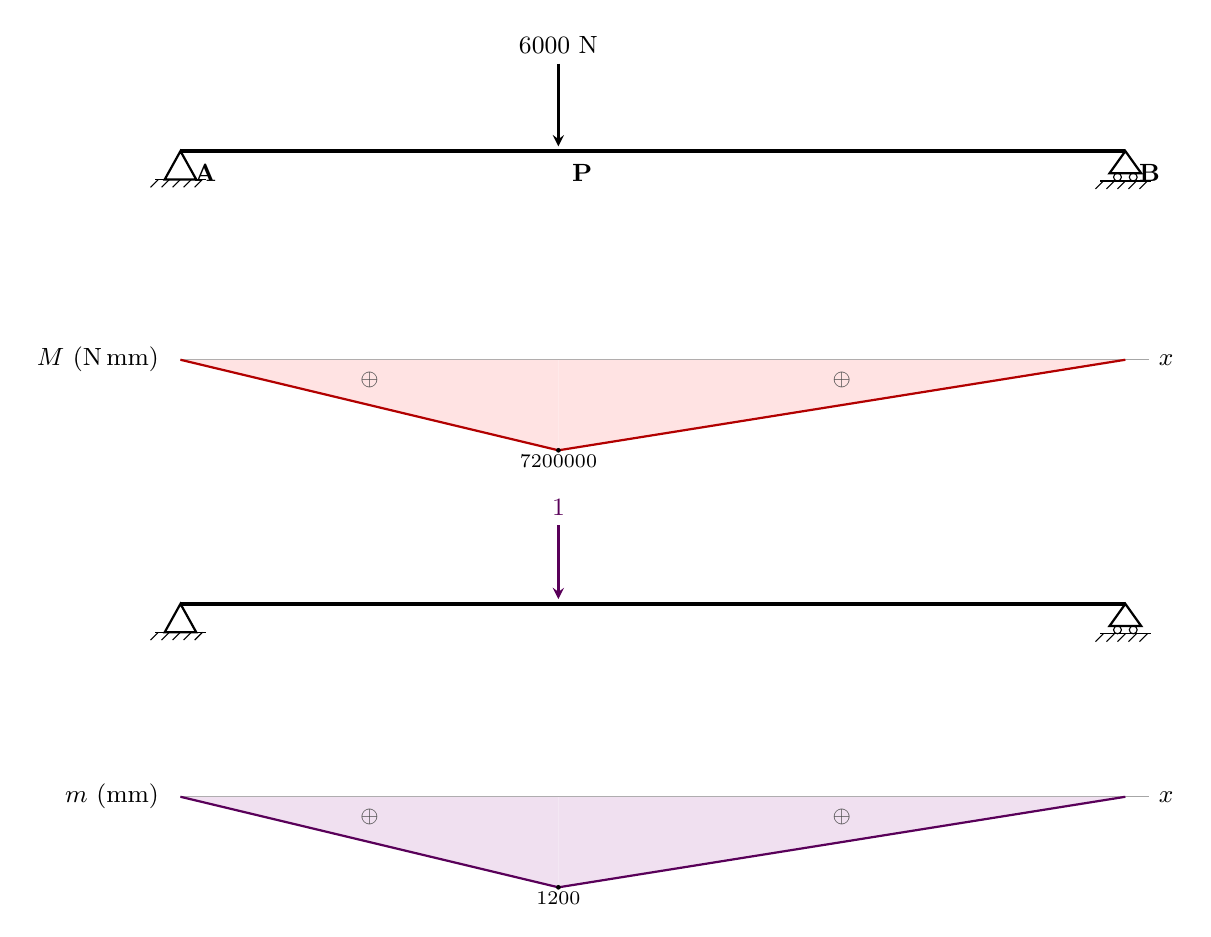
\begin{tikzpicture}
\draw[line width=1.6pt] (0,0.0000) -- (12.0000,0.0000);
% studium:at support A x=0 check=first
\draw[thick,fill=white] (0.0000,0.0000) -- (-0.2000,-0.3600) -- (0.2000,-0.3600) -- cycle;
\draw (-0.3200,-0.3600) -- (0.3200,-0.3600);
\draw (-0.2800,-0.3600) -- (-0.3800,-0.4600);
\draw (-0.1400,-0.3600) -- (-0.2400,-0.4600);
\draw (0.0000,-0.3600) -- (-0.1000,-0.4600);
\draw (0.1400,-0.3600) -- (0.0400,-0.4600);
\draw (0.2800,-0.3600) -- (0.1800,-0.4600);
% studium:at support B x=5000 check=first
\draw[thick,fill=white] (12.0000,0.0000) -- (11.8000,-0.2800) -- (12.2000,-0.2800) -- cycle;
\draw (11.9000,-0.3300) circle (0.05);
\draw (12.1000,-0.3300) circle (0.05);
\draw (11.6800,-0.3800) -- (12.3200,-0.3800);
\draw (11.7200,-0.3800) -- (11.6200,-0.4800);
\draw (11.8600,-0.3800) -- (11.7600,-0.4800);
\draw (12.0000,-0.3800) -- (11.9000,-0.4800);
\draw (12.1400,-0.3800) -- (12.0400,-0.4800);
\draw (12.2800,-0.3800) -- (12.1800,-0.4800);
% studium:at force 0 x=2000 check=tip
\draw[-stealth,thick,black] (4.8000,1.1100) -- (4.8000,0.0600);
\node[font=\small,anchor=south] at (4.8000,1.1100) {$6000$~\mbox{N}};
\node[font=\small\bfseries,anchor=north west] at (0.0500,-0.0500) {A};
\node[font=\small\bfseries,anchor=north west] at (4.8500,-0.0500) {P};
\node[font=\small\bfseries,anchor=north west] at (12.0500,-0.0500) {B};
\draw[gray!70] (0,-2.6500) -- (12.3000,-2.6500);
\fill[red!11] (0.0000,-2.6500) -- (0.0000,-2.6500) -- (4.8000,-3.8000) -- (4.8000,-2.6500) -- cycle;
\fill[red!11] (4.8000,-2.6500) -- (4.8000,-3.8000) -- (12.0000,-2.6500) -- (12.0000,-2.6500) -- cycle;
% studium:series M sx=0.0024 sy=1.597222222222222e-07 x0=0.0 y0=-2.65 sign=-1
\draw[thick,red!70!black] (0.0000,-2.6500) -- (4.8000,-3.8000);
\draw[thick,red!70!black] (4.8000,-3.8000) -- (12.0000,-2.6500);
% studium:end M
\node[font=\small,anchor=east] at (-0.15,-2.6500) {$M$ (N\,mm)};
\node[font=\small,anchor=west] at (12.3000,-2.6500) {$x$};
% studium:label M x=2000 side=both value=7200000
\fill (4.8000,-3.8000) circle (0.03);
\node[font=\scriptsize,anchor=north,inner sep=1.5pt] at (4.8000,-3.8000) {$7200000$};
\node[font=\footnotesize,gray!60!black] at (2.4000,-2.9087) {$\oplus$};
\node[font=\footnotesize,gray!60!black] at (8.4000,-2.9087) {$\oplus$};
\draw[line width=1.6pt] (0,-5.7500) -- (12.0000,-5.7500);
% studium:at support A x=0 check=first
\draw[thick,fill=white] (0.0000,-5.7500) -- (-0.2000,-6.1100) -- (0.2000,-6.1100) -- cycle;
\draw (-0.3200,-6.1100) -- (0.3200,-6.1100);
\draw (-0.2800,-6.1100) -- (-0.3800,-6.2100);
\draw (-0.1400,-6.1100) -- (-0.2400,-6.2100);
\draw (0.0000,-6.1100) -- (-0.1000,-6.2100);
\draw (0.1400,-6.1100) -- (0.0400,-6.2100);
\draw (0.2800,-6.1100) -- (0.1800,-6.2100);
% studium:at support B x=5000 check=first
\draw[thick,fill=white] (12.0000,-5.7500) -- (11.8000,-6.0300) -- (12.2000,-6.0300) -- cycle;
\draw (11.9000,-6.0800) circle (0.05);
\draw (12.1000,-6.0800) circle (0.05);
\draw (11.6800,-6.1300) -- (12.3200,-6.1300);
\draw (11.7200,-6.1300) -- (11.6200,-6.2300);
\draw (11.8600,-6.1300) -- (11.7600,-6.2300);
\draw (12.0000,-6.1300) -- (11.9000,-6.2300);
\draw (12.1400,-6.1300) -- (12.0400,-6.2300);
\draw (12.2800,-6.1300) -- (12.1800,-6.2300);
\draw[-stealth,thick,violet!70!black] (4.8000,-4.7500) -- (4.8000,-5.6900);
\node[font=\small,violet!70!black,anchor=south] at (4.8000,-4.7500) {$1$};
\draw[gray!70] (0,-8.2000) -- (12.3000,-8.2000);
\fill[violet!12] (0.0000,-8.2000) -- (0.0000,-8.2000) -- (4.8000,-9.3500) -- (4.8000,-8.2000) -- cycle;
\fill[violet!12] (4.8000,-8.2000) -- (4.8000,-9.3500) -- (12.0000,-8.2000) -- (12.0000,-8.2000) -- cycle;
% studium:series m sx=0.0024 sy=0.0009583333333333333 x0=0.0 y0=-8.2 sign=-1
\draw[thick,violet!70!black] (0.0000,-8.2000) -- (4.8000,-9.3500);
\draw[thick,violet!70!black] (4.8000,-9.3500) -- (12.0000,-8.2000);
% studium:end m
\node[font=\small,anchor=east] at (-0.15,-8.2000) {$m$ (mm)};
\node[font=\small,anchor=west] at (12.3000,-8.2000) {$x$};
% studium:label m x=2000 side=both value=1200
\fill (4.8000,-9.3500) circle (0.03);
\node[font=\scriptsize,anchor=north,inner sep=1.5pt] at (4.8000,-9.3500) {$1200$};
\node[font=\footnotesize,gray!60!black] at (2.4000,-8.4587) {$\oplus$};
\node[font=\footnotesize,gray!60!black] at (8.4000,-8.4587) {$\oplus$};
\end{tikzpicture}}%
\else
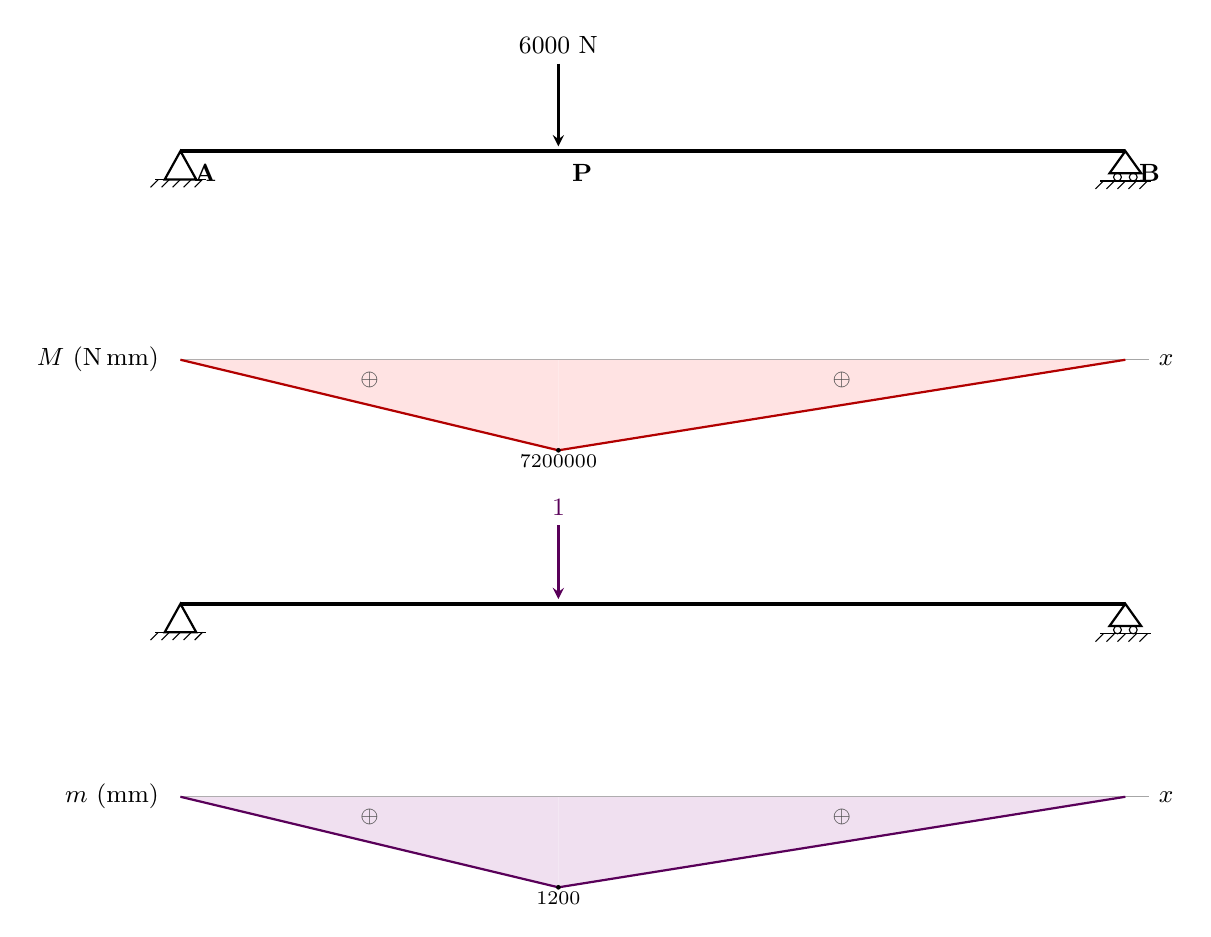
\begin{tikzpicture}
\draw[line width=1.6pt] (0,0.0000) -- (12.0000,0.0000);
% studium:at support A x=0 check=first
\draw[thick,fill=white] (0.0000,0.0000) -- (-0.2000,-0.3600) -- (0.2000,-0.3600) -- cycle;
\draw (-0.3200,-0.3600) -- (0.3200,-0.3600);
\draw (-0.2800,-0.3600) -- (-0.3800,-0.4600);
\draw (-0.1400,-0.3600) -- (-0.2400,-0.4600);
\draw (0.0000,-0.3600) -- (-0.1000,-0.4600);
\draw (0.1400,-0.3600) -- (0.0400,-0.4600);
\draw (0.2800,-0.3600) -- (0.1800,-0.4600);
% studium:at support B x=5000 check=first
\draw[thick,fill=white] (12.0000,0.0000) -- (11.8000,-0.2800) -- (12.2000,-0.2800) -- cycle;
\draw (11.9000,-0.3300) circle (0.05);
\draw (12.1000,-0.3300) circle (0.05);
\draw (11.6800,-0.3800) -- (12.3200,-0.3800);
\draw (11.7200,-0.3800) -- (11.6200,-0.4800);
\draw (11.8600,-0.3800) -- (11.7600,-0.4800);
\draw (12.0000,-0.3800) -- (11.9000,-0.4800);
\draw (12.1400,-0.3800) -- (12.0400,-0.4800);
\draw (12.2800,-0.3800) -- (12.1800,-0.4800);
% studium:at force 0 x=2000 check=tip
\draw[-stealth,thick,black] (4.8000,1.1100) -- (4.8000,0.0600);
\node[font=\small,anchor=south] at (4.8000,1.1100) {$6000$~\mbox{N}};
\node[font=\small\bfseries,anchor=north west] at (0.0500,-0.0500) {A};
\node[font=\small\bfseries,anchor=north west] at (4.8500,-0.0500) {P};
\node[font=\small\bfseries,anchor=north west] at (12.0500,-0.0500) {B};
\draw[gray!70] (0,-2.6500) -- (12.3000,-2.6500);
\fill[red!11] (0.0000,-2.6500) -- (0.0000,-2.6500) -- (4.8000,-3.8000) -- (4.8000,-2.6500) -- cycle;
\fill[red!11] (4.8000,-2.6500) -- (4.8000,-3.8000) -- (12.0000,-2.6500) -- (12.0000,-2.6500) -- cycle;
% studium:series M sx=0.0024 sy=1.597222222222222e-07 x0=0.0 y0=-2.65 sign=-1
\draw[thick,red!70!black] (0.0000,-2.6500) -- (4.8000,-3.8000);
\draw[thick,red!70!black] (4.8000,-3.8000) -- (12.0000,-2.6500);
% studium:end M
\node[font=\small,anchor=east] at (-0.15,-2.6500) {$M$ (N\,mm)};
\node[font=\small,anchor=west] at (12.3000,-2.6500) {$x$};
% studium:label M x=2000 side=both value=7200000
\fill (4.8000,-3.8000) circle (0.03);
\node[font=\scriptsize,anchor=north,inner sep=1.5pt] at (4.8000,-3.8000) {$7200000$};
\node[font=\footnotesize,gray!60!black] at (2.4000,-2.9087) {$\oplus$};
\node[font=\footnotesize,gray!60!black] at (8.4000,-2.9087) {$\oplus$};
\draw[line width=1.6pt] (0,-5.7500) -- (12.0000,-5.7500);
% studium:at support A x=0 check=first
\draw[thick,fill=white] (0.0000,-5.7500) -- (-0.2000,-6.1100) -- (0.2000,-6.1100) -- cycle;
\draw (-0.3200,-6.1100) -- (0.3200,-6.1100);
\draw (-0.2800,-6.1100) -- (-0.3800,-6.2100);
\draw (-0.1400,-6.1100) -- (-0.2400,-6.2100);
\draw (0.0000,-6.1100) -- (-0.1000,-6.2100);
\draw (0.1400,-6.1100) -- (0.0400,-6.2100);
\draw (0.2800,-6.1100) -- (0.1800,-6.2100);
% studium:at support B x=5000 check=first
\draw[thick,fill=white] (12.0000,-5.7500) -- (11.8000,-6.0300) -- (12.2000,-6.0300) -- cycle;
\draw (11.9000,-6.0800) circle (0.05);
\draw (12.1000,-6.0800) circle (0.05);
\draw (11.6800,-6.1300) -- (12.3200,-6.1300);
\draw (11.7200,-6.1300) -- (11.6200,-6.2300);
\draw (11.8600,-6.1300) -- (11.7600,-6.2300);
\draw (12.0000,-6.1300) -- (11.9000,-6.2300);
\draw (12.1400,-6.1300) -- (12.0400,-6.2300);
\draw (12.2800,-6.1300) -- (12.1800,-6.2300);
\draw[-stealth,thick,violet!70!black] (4.8000,-4.7500) -- (4.8000,-5.6900);
\node[font=\small,violet!70!black,anchor=south] at (4.8000,-4.7500) {$1$};
\draw[gray!70] (0,-8.2000) -- (12.3000,-8.2000);
\fill[violet!12] (0.0000,-8.2000) -- (0.0000,-8.2000) -- (4.8000,-9.3500) -- (4.8000,-8.2000) -- cycle;
\fill[violet!12] (4.8000,-8.2000) -- (4.8000,-9.3500) -- (12.0000,-8.2000) -- (12.0000,-8.2000) -- cycle;
% studium:series m sx=0.0024 sy=0.0009583333333333333 x0=0.0 y0=-8.2 sign=-1
\draw[thick,violet!70!black] (0.0000,-8.2000) -- (4.8000,-9.3500);
\draw[thick,violet!70!black] (4.8000,-9.3500) -- (12.0000,-8.2000);
% studium:end m
\node[font=\small,anchor=east] at (-0.15,-8.2000) {$m$ (mm)};
\node[font=\small,anchor=west] at (12.3000,-8.2000) {$x$};
% studium:label m x=2000 side=both value=1200
\fill (4.8000,-9.3500) circle (0.03);
\node[font=\scriptsize,anchor=north,inner sep=1.5pt] at (4.8000,-9.3500) {$1200$};
\node[font=\footnotesize,gray!60!black] at (2.4000,-8.4587) {$\oplus$};
\node[font=\footnotesize,gray!60!black] at (8.4000,-8.4587) {$\oplus$};
\end{tikzpicture}%
\fi
\fi
\endgroup
\par\nopagebreak
\studiumcaption{fig:e2-c07-w_carga_descentrada-trabajo-virtual}{Leyes flectoras real y virtual y carga unidad usadas en el cálculo energético.}
\end{minipage}\par\medskip

\textbf{Resultado e interpretación.}\[\fitmath{\delta \approx 4.0167364\,\mathrm{mm}}\]

La flecha depende de ambos brazos: a = 2000 mm y b = 3000 mm; no se puede usar PL\textsuperscript{3}/(48EI).

\par\textbf{Comprobación.} Aplica fuerza virtual para flecha y momento virtual para giro. Mantén las cargas auxiliares hasta después de derivar y separa los tramos de distinta rigidez.

\textbf{Límites.}\begin{itemize}\item se desprecia la deformación por cortante
\item el contraste de trabajos virtuales y elástica verifica el modelo adoptado, no su idoneidad física general\end{itemize}

\textbf{Errores frecuentes.}\begin{itemize}\item emplear un único EI donde la rigidez cambia
\item confundir el momento virtual unidad (para giros) con la carga virtual unidad (para flechas)
\item olvidar un tramo al integrar las leyes flectoras\end{itemize}

\end{studiumworked}

\Needspace{.3\textheight}

\begin{studiumworked}{PRB-0236}

\section{PRB-0236 · Tensión normal en la cara girada}

\textbf{Enunciado.} En un estado plano $\sigma_x$ = -135 MPa, $\sigma_y$ = -35 MPa y $\tau_{xy}$ = +50 MPa. Halle las tensiones sobre caras giradas -30 grados respecto al eje x, las tensiones principales y el ángulo principal. Use el convenio de Mohr de la ULE y dibuje el círculo.

\par\medskip\noindent\begin{tabular}{@{}p{.18\linewidth}p{.26\linewidth}p{.48\linewidth}@{}}
\toprule Símbolo & Valor y unidad & Significado\\\midrule
$\sigma_{x}$ & $-135\,\mathrm{MPa}$ & tensión normal x\\
$\sigma_{y}$ & $-35\,\mathrm{MPa}$ & tensión normal y\\
$\tau_{xy}$ & $50\,\mathrm{MPa}$ & cortante xy\\
$\sigma_{z}$ & $0\,\mathrm{MPa}$ & tensión normal z\\
$\sigma_{y\,fluencia}$ & $230\,\mathrm{MPa}$ & límite elástico uniaxial\\
$\theta$ & $-30{}^{\circ}$ & rotación física del plano\\
\bottomrule\end{tabular}\par\medskip

\textbf{Hipótesis.}\begin{itemize}\item Equilibrio cuasiestático y tensor de tensiones simétrico.
\item Las tensiones sigma xz y sigma yz son nulas; sigma z es principal fuera del plano.
\item Tracción positiva y convención de signos de la Universidad de León.\end{itemize}

\textbf{Modelo y desarrollo.}

Círculo de Mohr y tensiones equivalentes.\[\fitmath{R=\sqrt{\left(\frac{\sigma_x-\sigma_y}{2}\right)^2+\tau_{xy}^{2}},\quad\sigma_{1,2}=\frac{\sigma_x+\sigma_y}{2}\pm R}\]

\textbf{Procedimiento.}\begin{itemize}\item Formar la matriz del tensor de Cauchy y obtener las tensiones principales en el plano xy.
\item Añadir la tensión normal sigma z, ordenar los tres autovalores y calcular la máxima cortadura absoluta.
\item Obtener la tensión equivalente de von Mises y la magnitud equivalente de Tresca.
\item Aplicar las relaciones de transformación al elemento girado.
\item Si se proporciona el límite elástico, comparar ambos criterios de fluencia.\end{itemize}

\textbf{Cálculo de los pasos.}\begin{enumerate}

\item Centro del círculo en el plano xy.

\[\fitmath{\frac{-135 - 35}{2}\approx -85\,\mathrm{MPa}}\]

\item Radio del círculo de Mohr.

\[\fitmath{\sqrt{\left(\frac{-135 - -35}{2}\right)^{2} + 50^{2}}\approx 70.7106781\,\mathrm{MPa}}\]

\item Tensión principal mayor en el plano.

\[\fitmath{\frac{-135 - 35}{2} + \sqrt{\left(\frac{-135 - -35}{2}\right)^{2} + 50^{2}}\approx -14.2893219\,\mathrm{MPa}}\]

\item Tensión principal menor en el plano.

\[\fitmath{\frac{-135 - 35}{2} - \sqrt{\left(\frac{-135 - -35}{2}\right)^{2} + 50^{2}}\approx -155.710678\,\mathrm{MPa}}\]

\item Von Mises a partir de las componentes.

\[\fitmath{\frac{\sqrt{\left(-35 - 0\right)^{2} + \left(-135 - -35\right)^{2} + 6 \cdot 50^{2} + \left(0 - -135\right)^{2}}}{\sqrt{2}}\approx 149.080515\,\mathrm{MPa}}\]

\item Índice tensional de Tresca.

\[\fitmath{2 \left(25 \sqrt{2} + \frac{85}{2}\right)\approx 155.710678\,\mathrm{MPa}}\]

\item Tensión normal sobre la cara x prima.

Se separa la sustitución en auxiliares numéricos $a_i$, locales a este paso; las unidades corresponden al resultado final.

\[\fitmath{\begin{gathered}a_{1}=\cos{\left(2 \pi \left(-30\right) \frac{1}{180} \right)}\\a_{2}=\frac{a_{1} \left(-135 - -35\right)}{2}\\a_{3}=\sin{\left(2 \pi \left(-30\right) \frac{1}{180} \right)}\\a_{4}=50 a_{3}\\a_{5}=a_{2} + a_{4} + \frac{-135 - 35}{2}\\a_{5}\approx -153.30127\,\mathrm{MPa}\end{gathered}}\]

\item Tensión normal sobre la cara y prima.

Se separa la sustitución en auxiliares numéricos $a_i$, locales a este paso; las unidades corresponden al resultado final.

\[\fitmath{\begin{gathered}a_{1}=\cos{\left(2 \pi \left(-30\right) \frac{1}{180} \right)}\\a_{2}=\frac{a_{1} \left(-135 - -35\right)}{2}\\a_{3}=- a_{2}\\a_{4}=\sin{\left(2 \pi \left(-30\right) \frac{1}{180} \right)}\\a_{5}=50 a_{4}\\a_{6}=- a_{5}\\a_{7}=a_{3} + a_{6} + \frac{-135 - 35}{2}\\a_{7}\approx -16.6987298\,\mathrm{MPa}\end{gathered}}\]

\item Cortante sobre el plano girado.

\[\fitmath{- \frac{-135 - -35}{2} \sin{\left(2 \pi \left(-30\right) \frac{1}{180} \right)} + 50 \cos{\left(2 \pi \left(-30\right) \frac{1}{180} \right)}\approx -18.3012702\,\mathrm{MPa}}\]

\item Coeficiente de seguridad de von Mises.

\[\fitmath{\frac{230}{\frac{1}{2} \sqrt{2} \sqrt{\left(85 - 50 \sqrt{2}\right)^{2} + 20000 + \left(-85 - 50 \sqrt{2}\right)^{2}}}\approx 1.54279048}\]

\item Coeficiente de seguridad de Tresca.

\[\fitmath{\frac{230}{50 \sqrt{2} + 85}\approx 1.47709844}\]

\item Respuesta principal: comprobación final.

Se separa la sustitución en auxiliares numéricos $a_i$, locales a este paso; las unidades corresponden al resultado final.

\[\fitmath{\begin{gathered}a_{1}=\cos{\left(2 \pi \left(-30\right) \frac{1}{180} \right)}\\a_{2}=\frac{a_{1} \left(-135 - -35\right)}{2}\\a_{3}=\sin{\left(2 \pi \left(-30\right) \frac{1}{180} \right)}\\a_{4}=50 a_{3}\\a_{5}=a_{2} + a_{4} + \frac{-135 - 35}{2}\\a_{5}\approx -153.30127\,\mathrm{MPa}\end{gathered}}\]

\end{enumerate}

\textbf{Resultado e interpretación.}\[\fitmath{\begin{aligned}\sigma_{1,\mathrm{plano}} &\approx -14{,}29\,\mathrm{MPa},\quad \sigma_{2,\mathrm{plano}} \approx -155{,}7\,\mathrm{MPa}\\\sigma_{VM} &\approx 149{,}1\,\mathrm{MPa},\quad \sigma_{Tresca} \approx 155{,}7\,\mathrm{MPa}\\\sigma_{x\prime} \approx -153{,}3\,\mathrm{MPa}\end{aligned}}\]

La tensión principal mayor puede seguir siendo compresiva; el signo del ángulo requiere resolver el cuadrante con atan2.

\par\textbf{Comprobación.} Incluye la tercera tensión principal al evaluar Tresca y von Mises. Comprueba los invariantes antes y después de girar los ejes.

\textbf{Límites.}\begin{itemize}\item El motor solo admite cortante xy y la tensión normal z; no modela cortantes xz e yz distintos de cero.
\item El criterio de plastificación es aplicable a materiales metálicos dúctiles e isótropos.
\item Las comprobaciones reproducen el modelo indicado, no su validez constitutiva fuera del régimen elástico.\end{itemize}

\textbf{Errores frecuentes.}\begin{itemize}\item Confundir la máxima cortadura del plano xy con la máxima cortadura absoluta del tensor tridimensional.
\item Olvidar el signo de tau xy al transformar las componentes a otro plano.
\item Aplicar Tresca sin incluir la tercera tensión principal.\end{itemize}

\end{studiumworked}

\chapter{Soluciones del simulacro 4}

\objetivos{Contrasta primero el modelo y después las cifras; aplica la rúbrica del enunciado.}

\Needspace{.3\textheight}

\begin{studiumworked}{PRB-0153}

\section{PRB-0153 · Distorsión}

\textbf{Enunciado.} Una chapa de 7075 ($E = 71{,}7$ GPa, $\nu = 0{,}33$) trabaja a cortadura pura con una tensión tangencial de 50 MPa. Calcule el módulo transversal $G$ y la distorsión $\gamma$.

\par\medskip\noindent\begin{tabular}{@{}p{.18\linewidth}p{.26\linewidth}p{.48\linewidth}@{}}
\toprule Símbolo & Valor y unidad & Significado\\\midrule
$E$ & $71700.0\,\mathrm{MPa}$ & módulo de Young\\
$\nu$ & $0.33$ & coeficiente de Poisson\\
$\tau$ & $50\,\mathrm{MPa}$ & tensión tangencial\\
\bottomrule\end{tabular}\par\medskip

\textbf{Hipótesis.}\begin{itemize}\item material isótropo elástico lineal
\item cortadura pura\end{itemize}

\textbf{Modelo y desarrollo.}

Módulo transversal y distorsión.\[\fitmath{\gamma = \frac{\tau}{G},\quad G = \frac{E}{2(1+\nu)}}\]

\textbf{Procedimiento.}\begin{itemize}\item El módulo transversal es $G = E/[2(1+\nu)]$.
\item La distorsión es $\gamma = \tau/G$.\end{itemize}

\textbf{Cálculo de los pasos.}\begin{enumerate}

\item Módulo transversal.

\[\fitmath{\frac{71700.0}{2 \left(0.33 + 1\right)}\approx 26955\,\mathrm{MPa}}\]

\item Distorsión.

\[\fitmath{\frac{50}{71700.0 \frac{1}{2 \left(0.33 + 1\right)}}\approx 1.855\times10^{-3}\,\mathrm{rad}}\]

\end{enumerate}

\textbf{Resultado e interpretación.}\[\fitmath{G \approx 26{,}95\ \mathrm{GPa},\qquad \gamma \approx 1{,}855\times 10^{-3}\ \mathrm{rad}}\]

La distorsión es de unos $0{,}11$ grados.

\par\textbf{Comprobación.} Distingue tensión, deformación y desplazamiento. Comprueba el signo de la contracción transversal y la definición de cortadura ingenieril.

\textbf{Límites.}\begin{itemize}\item solo isótropos\end{itemize}

\textbf{Errores frecuentes.}\begin{itemize}\item usar $G = E/2$ sin el factor $1+\nu$\end{itemize}

\end{studiumworked}

\Needspace{.3\textheight}

\begin{studiumworked}{PRB-0207}

\section{PRB-0207 · Flexión compuesta con compresión}

\textbf{Enunciado.} Una sección rectangular de 80 \ensuremath{\times} 160 mm trabaja bajo N = -120 kN (compresión) y M\_z = -2,4 kN·m. Dibuje la sección y determine las tensiones extremas y si existe alguna fibra traccionada. Calcule el eje neutro y discuta si cruza la sección.

\par\medskip\noindent\begin{tabular}{@{}p{.18\linewidth}p{.26\linewidth}p{.48\linewidth}@{}}
\toprule Símbolo & Valor y unidad & Significado\\\midrule
$b_{1}$ & $80\,\mathrm{mm}$ & anchura de rectángulo\\
$h_{1}$ & $160\,\mathrm{mm}$ & altura de rectángulo\\
$N$ & $-120000.0\,\mathrm{N}$ & esfuerzo aplicado con signo\\
$Mz$ & $-2400000.0\,\mathrm{N\,mm}$ & esfuerzo aplicado con signo\\
\bottomrule\end{tabular}\par\medskip

\textbf{Hipótesis.}\begin{itemize}\item sección prismática y coordenadas y/z declaradas
\item tensiones elásticas lineales cuando se aplican N, M\_y, M\_z
\item cargas y dimensiones expresadas en N y mm\end{itemize}

\textbf{Modelo y desarrollo.}

Momentos geométricos y ley de Navier.\[\fitmath{A = \sum_i A_i,\quad y_G = \frac{\sum_i A_i y_i}{A},\quad I_z = \sum_i (I_{z,i}+A_i d_i^2)}\]

Flexión compuesta en ejes generales.\[\fitmath{\sigma_x = \frac{N}{A}+\frac{(M_z I_y-M_y I_{yz})y+(M_y I_z-M_z I_{yz})z}{I_y I_z-I_{yz}^{2}}}\]

\textbf{Procedimiento.}\begin{itemize}\item La figura establece qué partes pertenecen a la sección, la dirección de y y z y las dimensiones en milímetros.
\item El área total suma las áreas macizas y resta los huecos; los primeros momentos proporcionan las coordenadas del centroide.
\item Calcular I\_z por suma de las inercias propias de las piezas más A\_i por el cuadrado de cada distancia a G (Steiner).
\item El verificador geométrico de Studium contrasta las inercias por otra vía: integración directa sobre los contornos.
\item La tensión normal combina N/A y la flexión alrededor de los ejes centrales; si I\_yz no es cero se conserva en la relación general.
\item Determinar las fibras de tensión extrema evaluando la distribución lineal en los vértices y representar las zonas de compresión y tracción.
\item Como las dos tensiones extremas son negativas, la sección entera trabaja a compresión y el eje neutro no la atraviesa.\end{itemize}

\textbf{Cálculo de los pasos.}\begin{enumerate}

\item Área algebraica de la sección, descontando los huecos.

\[\fitmath{\left(80 - 0\right) \left(160 - 0\right)\approx 12800\,\mathrm{mm^2}}\]

\item Centroide en el eje vertical mediante primeros momentos.

\[\fitmath{\frac{\left(0 + 160\right) \left(80 - 0\right) \left(160 - 0\right)}{2 \left(80 - 0\right) \left(160 - 0\right)}\approx 80\,\mathrm{mm}}\]

\item Momento de inercia I\_z mediante el teorema de Steiner.

Se separa la sustitución en auxiliares numéricos $a_i$, locales a este paso; las unidades corresponden al resultado final.

\[\fitmath{\begin{gathered}a_{1}=\frac{\left(80 - 0\right) \left(160 - 0\right)^{3}}{12}\\a_{2}=\left(\left(-1\right) 80 + \frac{0 + 160}{2}\right)^{2}\\a_{3}=a_{2} \left(80 - 0\right) \left(160 - 0\right)\\a_{4}=a_{1} + a_{3}\\a_{4}\approx 27306667\,\mathrm{mm^4}\end{gathered}}\]

\item Tensión extrema: axil y flexión con el convenio declarado.

\[\fitmath{- \frac{525}{32}\approx -16.40625\,\mathrm{MPa}}\]

\end{enumerate}

\textbf{Resultado e interpretación.}\[\fitmath{\begin{gathered}y_G \approx 80\ \mathrm{mm}\\I_z \approx 27306667\ \mathrm{mm^4}\\\sigma_{\max} \approx -2{,}34375\ \mathrm{MPa}\\\sigma_{\min} \approx -16{,}40625\ \mathrm{MPa}\end{gathered}}\]

Ambos extremos de tensión son negativos: toda la sección permanece comprimida; no se debe inventar una zona de tracción.

\par\textbf{Comprobación.} Fija los ejes centroidales y el signo del axil y del flector. Comprueba la posición del eje neutro y la fibra extrema.

\textbf{Límites.}\begin{itemize}\item no se analizan plastificación, pandeo ni tensiones locales en uniones\end{itemize}

\textbf{Errores frecuentes.}\begin{itemize}\item Tomar la tensión axial como tracción pese al signo negativo.
\item Declarar que hay eje neutro interior sin comprobar el cambio de signo.\end{itemize}

\end{studiumworked}

\Needspace{.3\textheight}

\begin{studiumworked}{PRB-0212}

\section{PRB-0212 · Cajón cerrado cuadrado}

\textbf{Enunciado.} Un cajón cerrado cuadrado tiene línea media de 90 \ensuremath{\times} 90 mm, espesor 1,5 mm, torsor de +900 N·m, G = 26 955 MPa y longitud 800 mm. Obtenga q, la tensión tangencial, J y el giro. Dibuje el contorno y el sentido del flujo. [E2-C05:p\_cajon\_cuadrado]

\par\medskip\noindent\begin{tabular}{@{}p{.18\linewidth}p{.26\linewidth}p{.48\linewidth}@{}}
\toprule Símbolo & Valor y unidad & Significado\\\midrule
$M_{x}$ & $900000\,\mathrm{N\,mm}$ & torsor positivo ULE\\
$G$ & $26955\,\mathrm{MPa}$ & módulo transversal\\
$L$ & $800\,\mathrm{mm}$ & longitud de referencia\\
$t_{1}$ & $1.5\,\mathrm{mm}$ & inferior\\
$t_{2}$ & $1.5\,\mathrm{mm}$ & derecha\\
$t_{3}$ & $1.5\,\mathrm{mm}$ & superior\\
$t_{4}$ & $1.5\,\mathrm{mm}$ & izquierda\\
\bottomrule\end{tabular}\par\medskip

\par\medskip\noindent\begin{minipage}{\linewidth}\centering
\begin{tikzpicture}[>=Stealth]
\coordinate (A) at (0.00000,0.00000);
\fill (A) circle (1.5pt) node[above right,font=\small]{A};
\coordinate (B) at (3.00000,0.00000);
\fill (B) circle (1.5pt) node[above right,font=\small]{B};
\coordinate (C) at (3.00000,-3.00000);
\fill (C) circle (1.5pt) node[above right,font=\small]{C};
\coordinate (D) at (0.00000,-3.00000);
\fill (D) circle (1.5pt) node[above right,font=\small]{D};
\draw[->,very thick,studiumBlue] (A) -- (B) node[midway,fill=white,font=\small]{$t_1$};
\draw[->,very thick,studiumBlue] (B) -- (C) node[midway,fill=white,font=\small]{$t_2$};
\draw[->,very thick,studiumBlue] (C) -- (D) node[midway,fill=white,font=\small]{$t_3$};
\draw[->,very thick,studiumBlue] (D) -- (A) node[midway,fill=white,font=\small]{$t_4$};
\draw[->] (-1,.3)--(-.2,.3) node[above]{$z$};
\draw[->] (-1,.3)--(-1,-.5) node[left]{$y$};
\end{tikzpicture}
\par\small Nudos $(z,y)$ en mm: $A=(0,0)$; $B=(90,0)$; $C=(90,90)$; $D=(0,90)$.
\par\small Flechas: sentido positivo de $q(s)$; $s=0$ en el nudo inicial de cada pared.
\par\small Recorridos de célula: $A\to B\to C\to D$.
\par\normalsize\end{minipage}\par\medskip

\textbf{Hipótesis.}\begin{itemize}\item torsión pura de Saint-Venant; sección prismática
\item paredes delgadas de línea media especificada; G homogéneo
\item torsor positivo antihorario en la cara vista según ULE\end{itemize}

\textbf{Modelo y desarrollo.}

Torsión de pared delgada.\[\fitmath{J_{cerrada}=\frac{4A_m^2}{\oint ds/t},\qquad q=\frac{M_x}{2A_m}}\]

\textbf{Procedimiento.}\begin{itemize}\item Identificar si la sección está abierta, cerrada unicelular o bicelular; dibujar su geometría y espesores.
\item Para una célula cerrada emplear Bredt, con q constante y tau=q/t; el espesor variable afecta al giro.
\item Comprobar que el par exterior coincide con el que transmiten los flujos, si la sección es cerrada.
\item Calcular el giro total con theta = M\_x L/(G J), o con la compatibilidad de las celdas.
\item Las magnitudes de la solución se han contrastado mediante cálculo analítico y el motor estructural de Studium cuando éste ofrece esa comprobación.\end{itemize}

\textbf{Cálculo de los pasos.}\begin{enumerate}

\item Área de línea media.

\[\fitmath{\begin{aligned}
A_m &= a\,b\\
&\approx 8100\,\mathrm{mm}^{2}
\end{aligned}}\]

\item Flujo cortante de Bredt.

\[\fitmath{\begin{aligned}
q &= \frac{M_x}{2A_m}\\
&\approx 55{,}555556\,\mathrm{N/mm}
\end{aligned}}\]

\item Constante de torsión cerrada.

\[\fitmath{\begin{aligned}
J &= \frac{4A_m^2}{\sum_i \ell_i/t_i}\\
&\approx 1093500\,\mathrm{mm}^{4}
\end{aligned}}\]

\item Giro total entre extremos.

\[\fitmath{\begin{aligned}
\theta &= \frac{M_xL}{GJ}\\
&\approx 0{,}024427239\,\mathrm{rad}
\end{aligned}}\]

\item Tensión tangencial máxima.

\[\fitmath{\begin{aligned}
\tau_{\max} &= \frac{|q|}{t_{\min}}\\
&\approx 37{,}037037\,\mathrm{MPa}
\end{aligned}}\]

\end{enumerate}

\textbf{Resultado e interpretación.}\[\fitmath{\begin{gathered}J \approx 1093500\,\mathrm{mm}^{4}\\q \approx 55{,}555556\,\mathrm{N/mm}\\\tau_{\max} \approx 37{,}037037\,\mathrm{MPa}\\\theta_x \approx 0{,}024427239\,\mathrm{rad}\end{gathered}}\]

Para un contorno cerrado de pared delgada y espesor constante, el área encerrada y el perímetro determinan J.

\par\textbf{Comprobación.} Distingue secciones abiertas y cerradas: la constante torsional de tiras abiertas no es el momento polar. En multiceldas, exige equilibrio y giro compatible.

\textbf{Límites.}\begin{itemize}\item se desprecia el alabeo coaccionado, los radios de curvatura de las esquinas y los efectos locales
\item en secciones abiertas la tensión y el giro siguen la aproximación de tiras delgadas y no están verificados por un diagrama de flujo del motor\end{itemize}

\textbf{Errores frecuentes.}\begin{itemize}\item confundir tensión tangencial (N/mm\textsuperscript{2}) con flujo cortante (N/mm)
\item usar el área exterior en lugar de la encerrada por la línea media
\item sumar los dos flujos en la pared común en lugar de calcular su diferencia\end{itemize}

\end{studiumworked}

\Needspace{.3\textheight}

\begin{studiumworked}{PRB-0216}

\section{PRB-0216 · C abierto y centro de cortadura}

\textbf{Enunciado.} Un perfil C abierto tiene alma de 120 mm y alas de 70 mm (dimensiones de línea media), espesor 2 mm y cortante vertical de 4,8 kN. Calcule centroide, inercia, flujos máximos, tensión cortante máxima y localización del centro de cortadura respecto al alma.

\par\medskip\noindent\begin{tabular}{@{}p{.18\linewidth}p{.26\linewidth}p{.48\linewidth}@{}}
\toprule Símbolo & Valor y unidad & Significado\\\midrule
$V_{y}$ & $4800\,\mathrm{N}$ & cortante en eje y (ULE)\\
$V_{z}$ & $0\,\mathrm{N}$ & cortante en eje z (ULE)\\
$t_{1}$ & $2\,\mathrm{mm}$ & ala\_inferior\\
$t_{2}$ & $2\,\mathrm{mm}$ & alma\\
$t_{3}$ & $2\,\mathrm{mm}$ & ala\_superior\\
\bottomrule\end{tabular}\par\medskip

\par\medskip\noindent\begin{minipage}{\linewidth}\centering
\begin{tikzpicture}[>=Stealth]
\coordinate (P) at (1.75000,0.00000);
\fill (P) circle (1.5pt) node[above right,font=\small]{P};
\coordinate (Q) at (0.00000,0.00000);
\fill (Q) circle (1.5pt) node[above right,font=\small]{Q};
\coordinate (R) at (0.00000,-3.00000);
\fill (R) circle (1.5pt) node[above right,font=\small]{R};
\coordinate (S) at (1.75000,-3.00000);
\fill (S) circle (1.5pt) node[above right,font=\small]{S};
\draw[->,very thick,studiumBlue] (P) -- (Q) node[midway,fill=white,font=\small]{$t_1$};
\draw[->,very thick,studiumBlue] (Q) -- (R) node[midway,fill=white,font=\small]{$t_2$};
\draw[->,very thick,studiumBlue] (R) -- (S) node[midway,fill=white,font=\small]{$t_3$};
\draw[->] (-1,.3)--(-.2,.3) node[above]{$z$};
\draw[->] (-1,.3)--(-1,-.5) node[left]{$y$};
\end{tikzpicture}
\par\small Nudos $(z,y)$ en mm: $P=(70,0)$; $Q=(0,0)$; $R=(0,120)$; $S=(70,120)$.
\par\small Flechas: sentido positivo de $q(s)$; $s=0$ en el nudo inicial de cada pared.
\par\normalsize\end{minipage}\par\medskip

\textbf{Hipótesis.}\begin{itemize}\item comportamiento elástico lineal y pared delgada
\item cortante aplicado en el centro de cortadura, sin torsor exterior adicional
\item los booms, cuando se indican, soportan la tensión axial; paneles solo cortante
\item convenio ULE: y positivo hacia abajo, z a la derecha\end{itemize}

\textbf{Modelo y desarrollo.}

Equilibrio de pared delgada.\[\fitmath{\frac{\mathrm{d}q}{\mathrm{d}s}=-t(\alpha y+\beta z),\qquad \tau=\frac{q}{t}}\]

\textbf{Procedimiento.}\begin{itemize}\item Obtener área, centroide, I\_z, I\_y e I\_yz sumando aportaciones de pared y booms.
\item Determinar los gradientes de tensión axial con ambos cortantes y el producto de inercia; integrar dq/ds en cada pared.
\item Imponer continuidad y equilibrio en los nudos; en contornos abiertos q=0 en extremos libres y en celdas cerradas imponer compatibilidad de giros.
\item Localizar el centro de cortadura anulando el torsor debido al flujo; calcular la tensión máxima por |q(s)|/t en paredes y puntos críticos.
\item Las leyes completas q(s) por pared se indican a continuación; la coordenada s se mide desde el nudo inicial de cada pared y el sentido firmado sigue las flechas del diagrama. Los resultados geométricos se obtienen con la misma idealización de paredes y larguerillos del enunciado.
\item Pared ala\_inferior: q(s) = $\frac{4 s}{9}$ N/mm; s en mm desde su nudo inicial, con signo según el recorrido.
\item Pared alma: q(s) = $\frac{- s^{2} + 120 s}{270} + \frac{280}{9}$ N/mm; s en mm desde su nudo inicial, con signo según el recorrido.
\item Pared ala\_superior: q(s) = $\frac{280}{9} - \frac{4 s}{9}$ N/mm; s en mm desde su nudo inicial, con signo según el recorrido.
\item Pared crítica: alma; s = 60 mm desde su nudo inicial.\end{itemize}

\textbf{Cálculo de los pasos.}\begin{enumerate}

\item Área equivalente que soporta tensión axial.

\[\fitmath{2 \cdot 70 + 2 \cdot 70 + 2 \cdot 120\approx 520\,\mathrm{mm^2}}\]

\item Área que soporta esfuerzo normal en la idealización de paredes delgadas.

\[\fitmath{A=520\,\mathrm{mm^2}}\]

\item Propiedades geométricas de la sección (centroide y momentos de inercia).

\[\fitmath{z_G=18.8461538\,\mathrm{mm},\quad y_G=60\,\mathrm{mm}}\]

\item Momentos de inercia del modelo en los ejes centroidales.

\[\fitmath{I_z=1296000\,\mathrm{mm}^{4},\quad I_y=272641.026\,\mathrm{mm}^{4},\quad I_{yz}=0\,\mathrm{mm}^{4}}\]

\item Centro de cortadura a partir del equilibrio de los flujos; coordenadas del modelo.

\[\fitmath{z_C=-27.2222222\,\mathrm{mm},\quad y_C=60\,\mathrm{mm}}\]

\item Tensión máxima |q|/t en pared alma.

\[\fitmath{\tau_{\max}=\frac{|q(s_*)|}{t_{\mathrm{crit}}}\approx 22.2222222\,\mathrm{MPa}}\]

\end{enumerate}

\textbf{Resultado e interpretación.}\[\fitmath{\begin{aligned}
z_G &\approx 18.8461538\,\mathrm{mm}\\
y_G &\approx 60\,\mathrm{mm}\\
I_z &\approx 1296000\,\mathrm{mm}^{4}\\
I_y &\approx 272641.026\,\mathrm{mm}^{4}\\
I_{yz} &\approx 0\,\mathrm{mm}^{4}\\
|q(s_*)| &\approx 44.4444444\,\mathrm{N/mm}\\
s_* &\approx 60\,\mathrm{mm}\\
z_C &\approx -27.2222222\,\mathrm{mm}\\
y_C &\approx 60\,\mathrm{mm}\\
\tau_{\max} &\approx 22.2222222\,\mathrm{MPa}
\end{aligned}}\]

El centro de cortadura de una sección C abierta no coincide con el centroide; está fuera del contorno, al lado opuesto de las alas.

\par\textbf{Comprobación.} Conserva el sentido del recorrido de cada pared y distingue flujo de cortante y tensión. Si la carga no pasa por el centro de cortadura, incluye el torsor adicional.

\textbf{Límites.}\begin{itemize}\item hipótesis de pared delgada; no se evalúan alabeo restringido, pandeo ni uniones
\item la prueba automática de flujo representa equilibrio e hipótesis del modelo, no validación académica externa\end{itemize}

\textbf{Errores frecuentes.}\begin{itemize}\item confundir q (N/mm) y tau (N/mm\textsuperscript{2})
\item olvidar el producto de inercia en secciones no simétricas
\item aplicar una carga fuera del centro de cortadura y omitir el torsor inducido\end{itemize}

\end{studiumworked}

\Needspace{.3\textheight}

\begin{studiumworked}{PRB-0175}

\section{PRB-0175 · Momento de empotramiento}

\textbf{Enunciado.} Una viga de 4 m empotrada en un extremo y apoyada en el otro soporta una carga uniforme de 5 kN/m. Calcule la reacción en el apoyo, la reacción vertical en el empotramiento y el momento de empotramiento, en kN$\cdot$m.

\par\medskip\noindent\begin{tabular}{@{}p{.18\linewidth}p{.26\linewidth}p{.48\linewidth}@{}}
\toprule Símbolo & Valor y unidad & Significado\\\midrule
$q$ & $5\,\mathrm{N/mm}$ & carga uniforme\\
$L$ & $4000\,\mathrm{mm}$ & luz\\
\bottomrule\end{tabular}\par\medskip

\textbf{Hipótesis.}\begin{itemize}\item EI constante
\item solo flexión\end{itemize}

\textbf{Modelo y desarrollo.}

Momento de empotramiento.\[\fitmath{M_A = \frac{q\,L^{2}}{8}}\]

\textbf{Procedimiento.}\begin{itemize}\item La reacción en el apoyo es $X = 3qL/8$.
\item La reacción en el empotramiento es $qL - X = 5qL/8$.
\item El momento de empotramiento es $qL^2/8$.\end{itemize}

\textbf{Cálculo de los pasos.}\begin{enumerate}

\item Reacción en el apoyo.

\[\fitmath{3 \cdot 5 \cdot 4000 \cdot \frac{1}{8}\approx 7500\,\mathrm{N}}\]

\item Reacción en el empotramiento.

\[\fitmath{5 \cdot 5 \cdot 4000 \cdot \frac{1}{8}\approx 12500\,\mathrm{N}}\]

\item Momento de empotramiento en kN m.

\[\fitmath{\frac{5 \cdot 4000^{2}}{8 \cdot 1000000.0}\approx 10.0\,\mathrm{kN\,m}}\]

\end{enumerate}

\textbf{Resultado e interpretación.}\[\fitmath{X = 7{,}5\ \mathrm{kN},\quad R_A = 12{,}5\ \mathrm{kN},\quad M_A = 10{,}0\ \mathrm{kN\,m}}\]

La suma de las dos reacciones es la carga total, $20$ kN. Sin el apoyo, el momento de empotramiento sería $40$ kN m, cuatro veces mayor.

\par\textbf{Comprobación.} Aplica fuerza virtual para flecha y momento virtual para giro. Mantén las cargas auxiliares hasta después de derivar y separa los tramos de distinta rigidez.

\textbf{Límites.}\begin{itemize}\item EI constante\end{itemize}

\textbf{Errores frecuentes.}\begin{itemize}\item suponer que el apoyo toma la mitad de la carga\end{itemize}

\end{studiumworked}
